% concatenated from Caratheodory_Feb10.tex
\documentclass[11pt]{amsart}
\usepackage{amsmath}
\usepackage{amssymb}
\usepackage{caption}
\usepackage{subcaption}
\usepackage{float}
\usepackage[curve]{xypic}
\usepackage{cite}
\usepackage{enumitem}
\usepackage{color}
\usepackage{url}
\usepackage[usenames,dvipsnames]{xcolor}
\usepackage{graphicx}
\usepackage{verbatim}
\usepackage{tikz}
\usepackage[normalem]{ulem}
\usepackage{hyperref}

\setcounter{secnumdepth}{4}

\renewcommand{\arraystretch}{1.5}

\theoremstyle{plain}
\newtheorem{Theorem}{Theorem}[section]
\newtheorem{Corollary}[Theorem]{Corollary}
\newtheorem{Definition}[Theorem]{Definition}
\newtheorem{Example}[Theorem]{Example}
\newtheorem{Lemma}[Theorem]{Lemma}
\newtheorem{Proposition}[Theorem]{Proposition}
\newtheorem{Question}[Theorem]{Question}
\newtheorem{Solution}[Theorem]{Solution}
\newtheorem{conj}[Theorem]{Conjecture}

%\theoremstyle{remark}
\newtheorem{Remark}{Remark}
\newtheorem{Case}[Theorem]{Case}
\usetikzlibrary{patterns,arrows.meta}
\usetikzlibrary{arrows.meta}
\usepackage{pgfplots}



\newcommand{\Tei}{\mathcal{T}}
\newcommand{\HP}{\mathbb{H}}
\newcommand{\C}{\mathbb{C}}
\newcommand{\Mod}{\operatorname{Mod}}
\newcommand{\Q}{\mathcal{Q}}
\newcommand{\ou}{\mathbf{o}_u}
\newcommand{\ov}{\mathbf{o}_v}
\newcommand{\os}{\mathbf{o}_s}
\newcommand{\ot}{\mathbf{o}_t}

\newcommand{\WS}[1]{\footnote{\textcolor{red}{  Weixu: #1}}}

\newcommand{\TS}{\mathbf{S}}
\newcommand{\TL}{\mathbf{L}}
\newcommand{\TR}{\mathbf{R}}
\newcommand{\rot}{\mathbf{J}}


\usepackage{microtype}

\topmargin        -1.3cm
\evensidemargin  0.5cm
\oddsidemargin   0.5cm
\textheight       21.3cm
\textwidth       15.3cm

\topmargin        -1.3cm
\evensidemargin  0.5cm
\oddsidemargin   0.5cm
\textheight       21.3cm
\textwidth       15.3cm

\renewcommand{\baselinestretch}{1.2}


\title[Carath\'{e}odory metric]{The Carath\'{e}odory metric on Teichm\"uller space of genus two surface}
%\title{Carath\'{e}odory metrics on $\mathcal{T}_{0,6}$ and $\mathcal{T}_{2,0}$}
\author[K. Lin and W. Su]{Kejie Lin and Weixu Su}
%\date{\today}
\address{Kejie Lin: School of Mathematics, Sun Yat-sen University, Guangzhou 510275, China} \email{linkj23@mail2.sysu.edu.cn}

\address{Weixu Su: School of Mathematics, Sun Yat-sen University, Guangzhou 510275, China}
\email{suwx9@mail.sysu.edu.cn}

\begin{document}
\maketitle

\begin{abstract}
   Let $\Tei_{g,n}$ be the Teichm\"uller space of Riemann surfaces of genus $g$
   with $n$ punctures. It is conjectured  that the Teichm\"uller and Carath\'{e}odory  metrics agree on a Teichm\"{u}ller disk  if and only if all the zeros of the corresponding holomorphic quadratic differential are of even order.  The conjecture was proved by Gekhtman and Markovic for $\Tei_{0,5}\cong \Tei_{1,2}$. We confirm the  conjecture  for $\Tei_{2,0}\cong\Tei_{0,6}$.
\end{abstract}









\section{Introduction}

Let $\Tei_{g,n}$ be the Teichm\"{u}ller space of Riemann surfaces of genus $g$ with $n$ marked points. 
Throughout this paper, we assume that $3g-3+n\geq 2$. 
The Teichm\"uller space $\Tei_{g,n}$ is the (orbifold) universal cover of the moduli space of Riemann surfaces
 $\mathcal{M}_{g,n}$ and  is naturally a complex manifold of dimension $3g-3+n$. It is known that
 $\Tei_{g,n}$ can be realized as a bounded domain in $\C^{3g-3+n}$, by the Bers
 embedding \cite{Bers}. 
 



Let $\mathbb{H}$ be the upper half-plane, equipped with the Poincar\'e metric $$d_{\mathbb{H}}= \frac{|dz|}{2 \operatorname{Im} z}.$$
The \emph{Kobayashi metric} $d_{\mathcal{K}}$ on $\Tei_{g,n}$ is the largest metric so that every holomorphic map $$f: \mathbb{H}\rightarrow\Tei_{g,n}$$ is nonexpanding.
%$$d_{\mathcal{K}}(f(z),f(w)) \leq d_{\mathbb{H}}(z,w)$$
%for all $z,w\in \mathbb{H}$. 
Royden \cite{Royden1969} proved that the Kobayashi metric on $\Tei_{g,n}$ coincides with the Teichm\"{u}ller metric $d_{\mathcal{T}}$. 
Furthermore,  the Teichm\"uller metric is not homogeneous at any point and its isometry group is essentially the mapping class group.

Another natural metric on $\Tei_{g,n}$ satisfying the Schwarz-Pick inequality is the \emph{Carath\'{e}odory metric}, which can be defined as the smallest metric so that every holomorphic map $$F:  \Tei_ {g,n} \rightarrow \mathbb{H}$$ is nonexpanding.
Let $d_\mathcal{C}$ denote the \emph{Carath\'{e}odory metric} on $\Tei_{g,n}$.
 By the Schwarz Lemma, the inequality 
$$d_\mathcal{C} \leq d_\Tei$$ holds  on $\Tei_{g,n}$. 

A longstanding open  problem is whether the two metrics $d_\Tei$ and $d_\mathcal{C}$ agree on $\Tei_{g,n}$. Recently, Markovic \cite{Markovic2018} solved the problem. 

Teichm\"uller disks, also known as complex geodesics, are holomorphic isometric
 embeddings of the hyperbolic plane into Teichm\"uller space. There is a unique Teichm\"uller disc through any pair of distinct points in $\Tei_{g,n}$. Every Teichm\"uller disk is generated by a non-zero holomorphic quadratic differential $\phi$, with at most simple poles at the marked points.  

Let $$\tau^\phi: \mathbb{H} \rightarrow \Tei_{g,n}$$ 
be a Teichm\"uller disk. 
Kra \cite{Kra1981} proved that the two metrics $d_\Tei$ and $d_\mathcal{C}$ agree on $\tau^\phi$ if all the zeros of $\phi$ are of even order, 
see also McMullen \cite[Theorem 4.1]{McMullen2003}. 
\begin{Remark}
 Note that if a holomorphic quadratic differential $\phi$ vanishes at a marked point (puncture), then it is not necessary to require that it vanish of even order.
\end{Remark}

Markovic \cite{Markovic2018} established a criterion that says when the two metrics $d_\Tei$ and $d_\mathcal{C}$ agree on a Teichm\"uller disk. 
Then he used this criterion to show that  $d_\Tei$ and $d_\mathcal{C}$ disagree on certain Teichm\"uller disk in $\Tei_{0,5}$.
Since there exists a holomorphic and isometric embedding of $\Tei_{0,5}$  into $\Tei_{g,n}$, 
we have  $d_\Tei\neq d_\mathcal{C}$ on $\Tei_{g,n}$.

  An application of Markovic's result is to prove a folklore conjecture of Siu that the Teichm\"uller space is not biholomorphic to any bounded convex domain in $\C^{3g-3+n}$.  Note that Gupta and Seshadri 
 \cite[Theorem 1.1.]{GS2020} proved a related result that the Teichm\"uller space is not biholomorphically equivalent to any bounded domain in $\C^{3g-3+n}$ which is strictly locally convex at one boundary point. 

\medskip
 
A remaining problem is to classify Teichm\"{u}ller disks for which $d_\Tei = d_\mathcal{C}$.
This is equivalent  to classifying Teichm\"{u}ller disks that are holomorphic retracts of the Teichm\"uller space. Gekhtman and Markovic   \cite{GM2020} made the following conjecture.

\begin{conj}\label{conj:equl}
A Teichm\"uller disk  is a holomorphic retract if and only if it is generated by
a holomorphic quadratic differential all of whose zeros are of even order.
\end{conj}

Gekhtman and Markovic \cite[Theorem 1.2]{GM2020} proved the above conjecture for $\Tei_{0,5}\cong\Tei_{1,2}$. 
In this paper, we confirm the conjecture for $\Tei_{0,6}\cong\Tei_{2,0}$,
which is of complex dimension $3$. 


\begin{Theorem}\label{thm:main}
Let $\tau^{\phi}$ be a Teichm\"{u}ller disk in $ \Tei_{2,0}$.
    The Teichm\"uller metric and Carath\'{e}odory metric agree on $\tau^{\phi}$  if and only if  $\phi$ is a quadratic differential all of whose zeros are of even order.  
 \end{Theorem}
 
Equivalently, we show

\begin{Theorem}\label{thm:main2}
Let $\tau^{\phi}$ be a Teichm\"{u}ller disk in $\Tei_{0,6}$.
    The Teichm\"uller metric and Carath\'{e}odory metric agree on $\tau^{\phi}$  if and only if  either $\phi$ is a quadratic differential with no odd-order zeros, or $\phi$ is a quadratic differential with a simple zero located at a marked point.    
 \end{Theorem}
 
The proof of Theorem \ref{thm:main2}  follows the strategy developed by Gekhtman and Markovic \cite{Markovic2018, GM2020}. 
Due to Markovic's criterion, it suffices to classify Jenkins-Strebel differentials 
with at least one odd-order zero. In Section \ref{sec:classify}, by applying cylinder deformations or by interchanging the vertical and horizontal foliations if necessary, we prove  that Theorem \ref{thm:main2} can be reduced to  the case when $\phi$ is a staircase.

Assume that $\phi$ is a staircase surface and that the corresponding Teichm\"uller disk $\tau^{\phi}$
admits a holomoprhic retraction, say
$F: \mathcal{T}_{0,6} \to \mathbb{H}$. 
In Section \ref{sec:computation}, we use the Schwarz-Christoffel formula to compute $F$ on certain smooth paths of $\mathcal{T}_{0,6}$. The computation is explicit and it shows that  $F$ fails to be $C^2$-smooth, which leads to a contradiction. 
Our computational method generalizes Markovic's previous work on $L$-shaped pillowcases \cite{Markovic2018}. 





\begin{Remark}
By a result of Apisa and Wright \cite[Corollary 1.3]{AW2022},
Conjecture \ref{conj:equl} can be reduced to checking strata (and full loci of covers)
of genus zero quadratic differentials.
\end{Remark}





\subsection*{Acknowledgements} The authors are grateful to Lixin Liu for for his valuable suggestions. W. Su is partially
 supported by NSFC Grant No. 12371076.

\section{Teichm\"{u}ller disks and Orbit closures}

In this section, we introduce the notion of Teichm\"uller disk.
Then we recall the method of  Gekhtman and Markovic \cite{GM2020},
which reduces the classification of Teichm\"uller disks  to the case of Jenkins-Strebel differentials. 
Most of the  relevant materials can be found in \cite{GM2020}. 
See Gupta \cite{Gupta2020} for a survey on complex analytic aspect of Teichm\"uller space. 
For general background on Teichm\"uller theory and quadratic differentials, we refer to 
Hubbard \cite{Hubbard} and Strebel \cite{Strebel}.

\subsection{Teichm\"{u}ller disks and holomorphic retracts}
Let $S_{g,n}$ be an oriented surface of genus $g$
with $n$ marked points (punctures), where $3g-3+n\geq 2$. Let $\Tei_{g,n}$ be the Teichm\"{u}ller space of Riemann surfaces marked by $S_{g,n}$.
Let $\Mod_{g,n}$ be the mapping class group of $S_{g,n}$. The quotient $$\mathcal{M}_{g,n}=\Tei_{g,n}/\Mod_{g,n}$$ is the moduli space of Riemann surfaces. Let
 $$\pi:\Tei_{g,n}\rightarrow \mathcal{M}_{g,n}$$ be the natural projection.

Given $X\in \Tei_{g,n}$, a \emph{holomorphic quadratic differential} $\phi$ on $X$ is a $(2,0)$ tensor
locally given by 
$\phi=\phi(z) dz^2,$
where $\phi(z)$ is a holomorphic function. 
Let $Q(X)$ be the space of holomorphic quadratic differentials $\phi$ on $X$ such that the $L^1$-norm
$$\|\phi\| = \int_X |\phi|$$
is finite. Note that $\|\phi\|<\infty$ 
 if and only if $\phi$ has at most simple poles at the punctures. 
Any $\phi\in Q(X)$ 
induces a flat metric of finite area, which is also called a \emph{half-translation surface}. 

It is known that the  cotangent space of $\Tei_{g,n}$ at $X$
can be naturally identified with $Q(X)$ and the $L^1$-norm is dual to the Teichm\"uller norm. 
We denote the cotangent bundle by $Q\Tei_{g,n}$. 
A pair $(X,\phi)\in Q\Tei_{g,n}$ with $\phi\in Q(X)$ and $\phi\neq 0$ generates a holomorphic embedding
$$\tau^\phi: \HP \rightarrow \Tei_{g,n},$$ 
which is an isometry from the Poincar\'e metric on $\HP$
to the Teichm\"uller metric on $\Tei_{g,n}$. For each $\lambda\in \mathbb{H}$, 
the Riemann surface $X_\lambda= \tau^\phi(\lambda)$ is characterized by the property that the extremal quasiconformal map between $X$ and $X_\lambda$ has Beltrami differential 
$$\mu_\lambda = \left( \frac{i-\lambda}{i+\lambda}  \right) \frac{|\phi|}{\phi}.$$

In the natural coordinates associated with $\phi$, the extremal quasiconformal map is 
an affine map of the form $$z=x+iy \mapsto  x+\lambda y.$$ 
By abuse of notation, we write $$\tau^{\phi}(\lambda)=\left( \frac{i-\lambda}{i+\lambda}  \right) \frac{|\phi|}{\phi}.$$ 
We call $\tau^{\phi}$ the \emph{Teichm\"{u}ller disk} generated by $\phi$.
%Without loss of generality, we may assume that $\|\phi\|=1$.
Note that $\tau^\phi\left( i \cdot \mathbb{R}_+ \right)$ is the Teichm\"uller geodesic
in the direction of $\phi$.


\begin{Definition}[Holomorphic retract]
  Let $\tau^\phi: \HP \rightarrow \Tei_{g,n}$ be a Teichm\"uller disk. 
We say that $\tau^{\phi}$ is a \emph{holomorphic retract} of $\Tei_{g,n}$ if 
there exists a holomorphic map $F : \Tei_{g,n} \to \HP$ such that $$F\circ \tau^\phi=\mathrm{id}_\HP.$$
Any holomorphic map  $F : \Tei_{g,n} \to \HP$ satisfies the above property is called a holomorphic retraction of $\tau^\phi$.
\end{Definition}

The following lemma states that classifying Teichm\"uller disks for which $d_\Tei = d_\mathcal{C}$ is equivalent to classifying holomorphic retracts of $\Tei_{g,n}$.
See \cite[Lemma 1.3]{GM2020}.
\begin{Lemma}
 The Kobayashi and Carath\'{e}odory metrics agree on a Teichm\"{u}ller disk $\tau^{\phi}$ if and only if $\tau^{\phi}$ is a holomorphic retract of $\Tei_{g,n}$.
\end{Lemma}





\subsection{Orbit closures}


There is a natural $\operatorname{GL}_2^+(\mathbb{R})$-action on $Q\Tei_{g,n}$ 
that commutes with 
the action of $\operatorname{Mod}_{g,n}$.  One can define a quadratic differential
$\phi$ by gluing a polygon $P$ along sides in pairs, in a way that each side of $P$
belongs to exactly one pair and the two sides in each pair are parallel and of the
same length. If $A\in \operatorname{GL}_2^+(\mathbb{R})$, then $A$ acts on $P$
as an affine transformation. By definition,  $A \cdot \phi$ is the quadratic differential obtained by gluing $A\cdot P$ in the same pattern as that for $P$. 
%Denote the $\operatorname{GL}_2^+(\mathbb{R})$ action by
%$$\widetilde{\tau^\phi} : \operatorname{GL}_2^+(\mathbb{R}) \to Q\Tei_{g,n}.$$

Let $p: Q\Tei_{g,n} \to \Tei_{g,n}$ be the natural projection. 
For any $(X,\phi) \in  Q\Tei_{g,n}$, the image of $A \cdot (X,\phi)$ under $p$
remains the same if and only if we multiply $A$ by $\mathbb{C}^*=\mathbb{C}\setminus\{0\}$. 
Note that $\mathbb{H} \cong  \mathbb{C}^* \backslash \operatorname{GL}_2^+(\mathbb{R})$. In fact, we can identify $\mathbb{H}$
as a subgroup of $\operatorname{GL}_2^+(\mathbb{R})$:

$$\mathbb{H} \cong\left\{\begin{pmatrix}
    1 & \operatorname{Re} \lambda\\
    0 & \operatorname{Im} \lambda
\end{pmatrix} \ : \  \lambda\in \mathbb{H} \right\}.$$

In complex coordinates, the action of $\begin{pmatrix}
    1 & \operatorname{Re} \lambda\\
    0 & \operatorname{Im} \lambda
\end{pmatrix}$ is given by 
$$x+i y \mapsto x + \lambda y.$$
So the Beltrami differential is $$\left( \frac{i-\lambda}{i+\lambda}  \right) \frac{|\phi|}{\phi},$$
which coincides with $\tau^\phi(\lambda)$ defined before.


Let $Q\mathcal{M}_{g,n} = Q\Tei_{g,n} / \Mod_{g,n}$ be the moduli space of holomorphic quadratic differentials. 
We also use $\pi$ to denote the natural projection $ Q\Tei_{g,n} \to Q\mathcal{M}_{g,n}$. The $\operatorname{GL}_2^+(\mathbb{R})$-action on $Q\Tei_{g,n}$ 
induces an action of $\operatorname{GL}_2^+(\mathbb{R})$ on $Q\mathcal{M}_{g,n}$.
Given $(X,\phi)\in Q\mathcal{M}_{g,n}$, we denote by $\operatorname{GL}_2^+(\mathbb{R}) \cdot \phi$ the $\operatorname{GL}_2^+(\mathbb{R})$ orbit of $(X,\phi)$. 
Let $\overline{\operatorname{GL}_2^+(\mathbb{R}) \cdot \phi}$ be the orbit closure in a stratum of $Q\mathcal{M}_{g,n}$.

The next result is very useful, proved by Gekhtman and Markovic \cite[Lemma 2.2]{GM2020}.

\begin{Proposition}\label{lem:GM-orbit}
Let $\phi$ be a quadratic differential. 
    If $\phi$ generates a Teichm\"uller disk $\tau^\phi$ that is a holomorphic retract of $\mathcal{T}_{g,n}$, so does every  element in the  orbit closure  $\overline{\operatorname{GL}_2^+(\mathbb{R}) \cdot \phi}$.
\end{Proposition}




Let 
$ \kappa =(\kappa_1, \cdots, \kappa_m)$ be an integral vector where $\kappa_i \geq -1$, $i = 1,...,m$, and satisfy $\sum\limits_{i=1}^{m} \kappa_i =4g-4.$ 
Denote by $\mathcal{Q}(\kappa)$ the stratum of quadratic differentials $(X,\phi)$ in
$Q\mathcal{M}_{g,n}$ consisting of $\phi$ with $m$ distinct zeros or poles of multiplicities $\kappa_1, \cdots, \kappa_m$. 


The horocycle flow action $h_t : \mathcal{Q}(\kappa) \rightarrow \mathcal{Q}(\kappa)$ 
is defined  as the restriction of the $\operatorname{GL}_2^+(\mathbb{R})$-action to the subgroup
$$H=\left\{\begin{pmatrix}
    1 & t\\
    0 & 1
\end{pmatrix} \ : \  t\in \mathbb{R} \right\}.$$
We refer to \cite{CW2022} for a comprehensive survey of the dynamics of
 the horocycle flow.

Let $\phi$ be a non-zero Jenkins-Strebel differential  in $Q\mathcal{M}_{0,6}$ with $k$ cylinders. A \emph{saddle connection} of $\phi$ is a geodesic segment connecting singularities (zeros or poles) of $\phi$, and
which does not contain any singularities in its interior. 
Let $\mathcal{F}(\phi)$ be the horizontal foliation
 of $\phi$, whose leaves are tangent to the directions  such that $\phi(z)dz^2>0$.   Denote the horizontal critical graph of $\phi$
by $\Gamma=\Gamma(\phi)$. 
We say that  $\phi$ or $\mathcal{F}(\phi)$ is \emph{Jenkins-Strebel}  if $\Gamma(\phi)$ is compact and the complement $X\setminus \Gamma(\phi)$  is a union of disjoint flat cylinders foliated by horizontal closed leaves. 


Smillie and Weiss \cite[Theorem 5]{SW2004} proved the following theorem. 

\begin{Theorem}\label{thm:SW}
Let $(X,\phi) \in \mathcal{Q}(\kappa)$. Then
\begin{enumerate}
  \item The  closure $\overline{H \cdot \phi}$ contains a Jenkins-Strebel differential $\psi\in  \mathcal{Q}(\kappa)$. 
  \item If $\phi$ has $k$ horizontal cylinders whose union is not dense in $S_{g,n}$,
  then there exists a Jenkins-Strebel differential $\psi$ in $\overline{H \cdot \phi}$ that has at least $k+1$ horizontal cylinders. 
\end{enumerate}   
\end{Theorem}
See \cite[\S 2.4]{GM2020} for details.

By Proposition \ref{lem:GM-orbit} and Theorem \ref{thm:SW}, Conjecture \ref{conj:equl}
can be reduced to the classification of Jenkins-Strebel differentials. 


\subsection{Markovic's criterion } 
Suppose that $\phi$ is a Jenkins-Strebel differential on $X$ that decomposes the surface into a finite number of horizontal cylinders $\Pi_{j}, j=1,\cdots,k$. 

Let $\mathbb{H}^k$ be the $k$-fold product of the upper half-plane $\mathbb{H}$. Following \cite[Section 4]{Markovic2018}, we define the \emph{Teichm\"uller polydisk} $$\mathcal{E}^\phi:\mathbb{H}^k\rightarrow \Tei_{g,n}$$ by associating 
each ${\lambda}= (\lambda_1, \cdots, \lambda_k)$ a Riemann surface $X_\lambda\in \Tei_{g,n}$ determined by the Beltrami differential  $$\mu_\lambda=\left( \frac{i-\lambda_j}{i+\lambda_j} \right) \frac{|\phi|}{\phi}$$ 
on each $\Pi_{j}$. 

\begin{Remark}
  It is known that (see \cite[Section 4]{Markovic2018}) $\mathcal{E}^\phi$ is a holomorphic embedding, but not proper.
\end{Remark}

Denote by $h_j$ the height of $\Pi_{j}$.
Note that each $\Pi_j$ is deformed into a new horizontal cylinder $\Pi_j(\lambda)$.
The circumference is preserved, while the height is scaled by a factor $\operatorname{Im} \lambda_j$. 
By gluing $\Pi_j(\lambda), i =1, \cdots, k$, we obtain a
new Jenkins-Strebel differential $\phi_\lambda$ on $X_\lambda$.



The following beautiful and important theorem provides a criterion to characterize Jenkins-Strebel differentials which generate Teichm\"uller disks 
that admit holomorphic retractions.  See \cite[Theorem 4.1]{GM2020}.

\begin{Theorem}[Markovic's criterion]\label{thm:GM-JS}
      Let $\phi\in Q(X)$ be a non-zero Jenkins-Strebel differential. Denote the area of the $j$-th cylinder of $\phi$ by $a_j$ . Let $\mathcal{E}^{\phi}:\mathbb{H}^k\rightarrow\Tei_{g,n}$ be the Teichm\"{u}ller polydisk associated with $\phi$. Then the Teichm\"{u}ller disk $\tau^{\phi}$ admits a holomorphic retraction  if and only if there exists a holomorphic map $\Phi:\Tei_{g,n}\rightarrow \mathbb{H}$ satisfying \begin{equation}\label{equ:criterion}
       \left(\Phi\circ \mathcal{E}^\phi\right)(\lambda)=\sum\limits_{j=1}^{k}a_j\lambda_j.
      \end{equation}
\end{Theorem}

As a corollary of Theorem \ref{thm:GM-JS}, if $\phi$ is a Jenkins-Strebel differential with $k$ cylinders and if $\phi$ generates a Teichm\"uller disk that admits a holomorphic retraction, then so does every quadratic differential in its $\mathbb{H}^k$ orbit.


Based on Theorem \ref{thm:GM-JS}, Gekhtman and Markovic proposed the program to solve Conjecture \ref{conj:equl} by showing that for any quadratic differential $\phi$ with an odd-order zero (not lie at a marked point), the orbit closure of $\phi$ contains a Jenkins-Strebel differential that does not satisfy the criterion \eqref{equ:criterion}. They carried out the program for $\Tei_{0,5}$ in \cite{GM2020}. 

In the remainder of this paper, we focus on $\Tei_{0,6}$. 







\section{Classification of Jenkins-Strebel differentials on $S_{0,6}$}
\label{sec:classify}


We adopt the following notation. Let  $\mathcal{Q}(\kappa)$ be a stratum of $Q\mathcal{M}_{0,6}$, where $\kappa=(\kappa_1, \cdots, \kappa_m)$.  If there are $j$ multiplicities say $\kappa_{1},\cdots, \kappa_{j}$ that are equal to some $n\in \mathbb{Z}$, then we denote $n^{j}$ instead of $(\kappa_{1},\cdots, \kappa_{j})$. For instance, $\mathcal{Q}(-1^4)$ denotes 
the stratum of quadratic differentials with four simple poles (without zeros),
and $\mathcal{Q}(2, -1^6)$ denotes 
the stratum of quadratic differentials with a single zero of order $2$ 
and six simple poles.
There are four strata in $Q\mathcal{M}_{0,6}$, as illustrated in the following table:

\bigskip

\begin{center}
\begin{tabular}{ |c |c |c| c | c| } 
  \hline
Case & (I) & (II) & (III) & (IV)  \\ 
  \hline
 Stratum &  $\Q(1^2, -1^6)$ & $\Q(2, -1^6)$ & $\Q(1, -1^5)$ & $\Q(-1^4)$ \\ 
  \hline
\end{tabular}
\end{center}

\bigskip

A Jenkins-Strebel differential  that is obtained by taking the double of a rectilinear polygon (whose sides are parallel to the coordinate axes) is called a \emph{pillowcase}. 
A \emph{staircase (surface)} on $S_{0,6}$ is the double of a staircase-shaped polygon  illustrated  in Figure   
\ref{fig:staircase}. It is a Jenkins-Strebel differential with two simple zeros and six simple poles.
This concept can be extended to flat surfaces on $S_{0,n}$ for any $n\geq 5$. 

\begin{figure}[h]\label{fig:staircase}
   \centering
   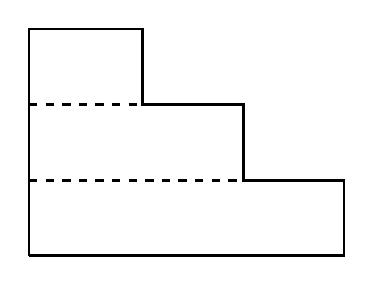
\begin{tikzpicture}[line width=1pt,scale=0.8]
     \draw (-5.7,0)--(-0.7,0)--(-0.7,1.2)--(-2.3,1.2)--(-2.3,2.4)--(-3.9,2.4)--(-3.9,3.6)--(-5.7,3.6)--(-5.7,0);
        \draw[dashed] (-5.7,1.2)--(-2.3,1.2);
        \draw[dashed] (-5.7,2.4)--(-3.9,2.4);
    \end{tikzpicture}
    \caption{The double of the polygon is called a staircase.}
    \label{fig:staircase}
\end{figure}

The first step to prove Theorem \ref{thm:main2} is to classify Jenkins-Strebel differentials on $S_{0,6}$.  In this section, we show that the problem can be reduced to 
staircase surfaces.




\begin{Remark}
Staircase surfaces on $S_{0,7}$ are used by Bourque and Rafi \cite{BourqueRafi} to construct  non-convex Teichm\"uller geodesic balls. 
  Staircase surfaces on $S_{0,n}$ (and the moduli space) are studied by Weber and Wolf \cite{WW98} for finding minimal surfaces. 
\end{Remark}






If $\phi$ is a Jenkins-Strebel differential with $k$ horizontal cylinders, then 
 $\mathbb{H}^k$ acts on  $\phi$ through the Teichm\"uller polydisk associated with $\phi$. 
Throughout what follows, we denote by
$$\rot=\begin{pmatrix}
    0 & -1\\
    1 & 0
\end{pmatrix}$$
the rotation matrix of the plane by angle $\frac{\pi}{2}$. The matrix $\rot$ acts on $\phi$ by interchanging the horizontal and vertical foliations.

This section contains many figures that serve to illustrate the proofs. We usually plot the trajectories of a quadratic differential on the plane, with the assumption that the point at infinity is a regular point.


\subsection{Case (I): $\phi \in \Q(1^2, -1^6)$.}\label{Case-I}
In this case, $\phi$ has two simple zeros and six simple poles.  
Most of this section will be devoted to this case. 
We shall classify $\phi$ according to the topological type of its critical graph $\Gamma$.
Denote the zeros of $\phi$ by $z_1$ and $z_2$. Denote the poles by $p_1, \cdots, p_5$ and $p_6$. 

\medskip
\noindent
{\bf Jenkins-Strebel differentials with three cylinders.}

\subsection*{Case (I-1):} \label{case-I-1} Each zero $z_i$ of $\phi$ is connected to itself by a horizontal saddle connection, and there is a horizontal saddle connection joining $z_i$ and a pole. 
There are three possibilities as shown in Figure \ref{fig:I-1},
which are referred to as type (a), (b) and (c), respectively. 
The surface is decomposed by $\Gamma$ into three cylinders, $\Pi_1, \Pi_2$ and $\Pi_3$,  which are arranged sequentially such that $\Pi_2$ separates $\Pi_1$ from $\Pi_3$. 
Denote their circumferences by $\ell_1,\ell_2$ and $\ell_3$.


\begin{figure}[h]
\centering

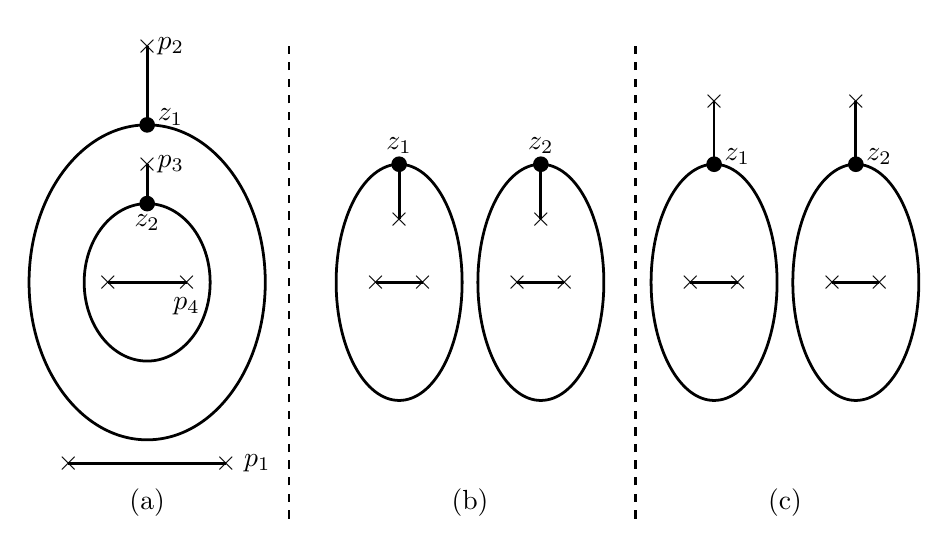
\begin{tikzpicture}[line width=1pt,scale=1]
%[every node/.style = {draw, circle, inner sep = 2pt}]
  % 圆形：圆心在 (0,0)，半径为 1.5cm
 % \node (A) at (0,0);
 
  \draw (-4.2,0) ellipse (1.5cm and 2cm);
  \node[ circle, fill=black,inner sep = 2pt] (A) at (-4.2, 2.0){};
  \node[right] at (-4.2, 2.1) {$z_1$};
  \draw (-4.2,2.0) to (-4.2,3.0);
   \node  at (-4.2, 3.0) {$\times$};
   \node  at (-3.9, 3.0) {$p_2$};
   \draw (-4.2,0) ellipse (0.8cm and 1.0cm);
   \node[ circle, fill=black,inner sep = 2pt] (A) at (-4.2, 1.0){};
   \node[below] at (-4.2, 1.0) {$z_2$};
   \draw (-4.2,1.0) to (-4.2,1.5);
   \node  at (-3.9, 1.5) {$p_3$};
   \node  at (-4.2, 1.5) {$\times$};
   \draw (-4.7,0) to (-3.7,0);
    \node  at (-4.7, 0){$\times$};
     \node at (-3.7, 0){$\times$};
     \node at (-3.7, -0.3){$p_4$};
     \draw (-5.2,-2.3) to (-3.2, -2.3);
      \node at (-5.2,-2.3){$\times$};
     \node  at (-3.2, -2.3){$\times$};
     \node at (-2.8, -2.3){$p_1$}; 
     \node  at (-4.2,-2.8) {(a)};
     \draw[dashed] (-2.4,-3)--(-2.4,3);
   % \caption(-4, -3){fig:a}
  % 椭圆：圆心在 (4,0)，x轴半径为 2cm，y轴半径为 1cm
  %\draw (4,0) ellipse (2cm and 1cm);
  %\caption{aaa}

%\lable{fig:a}
 \draw (-1.0,0) ellipse (0.8cm and 1.5cm);
 \draw (0.8,0) ellipse (0.8cm and 1.5cm);
 \draw (-1.0,1.5) to (-1.0,0.8);
 \draw (0.8,1.5) to (0.8, 0.8);
\node[ circle, fill=black,inner sep = 2pt] (A) at (-1.0, 1.5){};
\node[ circle, fill=black,inner sep = 2pt] (A) at (0.8, 1.5){};
\node[above] at (-1.0, 1.5) {$z_1$};
\node[above] at (0.8, 1.5) {$z_2$};
\node at (-1.0,0.8){$\times$};
\node  at(0.8, 0.8){$\times$};
\draw (-0.7,0) to (-1.3,0);
\node  at(-0.7,0){$\times$};
\node  at(-1.3,0){$\times$};
\draw (0.5,0) to (1.1,0);
\node  at(0.5,0){$\times$};
\node  at(1.1,0){$\times$};
\draw [dashed] (2,-3)--(2,3);
\node  at (-0.1,-2.8) {(b)};

\draw (3,0) ellipse (0.8cm and 1.5cm);
 \draw (4.8,0) ellipse (0.8cm and 1.5cm);
 \draw (3.0,1.5) to (3.0,2.3);
 \draw (4.8,1.5) to (4.8,2.3);
\node[ circle, fill=black,inner sep = 2pt] (A) at(3.0,1.5){};
\node[ circle, fill=black,inner sep = 2pt] (A) at (4.8,1.5){};
\node[right] at (3.0,1.6) {$z_1$};
\node[right] at (4.8,1.6) {$z_2$};
\node  at(3.0,2.3){$\times$};
\node  at(4.8,2.3){$\times$};
\draw (2.7,0) to (3.3,0);
\node  at(2.7,0){$\times$};
\node  at(3.3,0){$\times$};
\draw (4.5,0) to (5.1,0);
\node  at(4.5,0){$\times$};
\node  at(5.1,0){$\times$};
\node  at (3.9,-2.8) {(c)};
    %\draw (4,0) ellipse (2cm and 1cm);
\end{tikzpicture}
%\lable{fig:a}
\caption{Case (I-1): The crosses stand for simple poles and the black dots stand for zeros. The Jenkins-Strebel differential $\phi$ is decomposed by the critical graph into three cylinders.}
\label{fig:I-1}
\end{figure}

\subsubsection*{\textbf{(I-1-a):}} $\phi$ is of type (a).  
The circumferences of the cylinders satisfy $\ell_3 < \ell_2 < \ell_1$.


Now $\HP^3$ acts on $\phi$ through the Teichm\"uller polydisk $\mathcal{E}^\phi$. 
We  shear $\Pi_1$   appropriately so that there exists a vertical saddle connection ending at the poles $p_1$ and $p_2$. See Figure \ref{fig:I-1} (a) for the notation. More precisely, 
we take a saddle connection in the cylinder $\Pi_1$ connecting $p_1$ and $p_2$, which may not be vertical. However, we can use the horocycle flow action on $\Pi_1$ to shear the cylinder so that 
saddle connection is vertical. 

Similarly, we shear $\Pi_2$ appropriately so that there is a vertical saddle connection connecting $z_1$ to the pole $p_3$. Finally, we shear $\Pi_3$ appropriately so that there exists a vertical saddle connection joining  $z_2$ and the pole $p_4$. 
We obtain a quadratic differential $\psi$ that lies within the $\HP^3$-orbit of $\phi$. Moreover, $\psi$  is a staircase, obtained by doubling the polygon as illustrated in the first case of Figure  \ref{fig:I-1-new}.


\begin{figure}[h]
    \centering


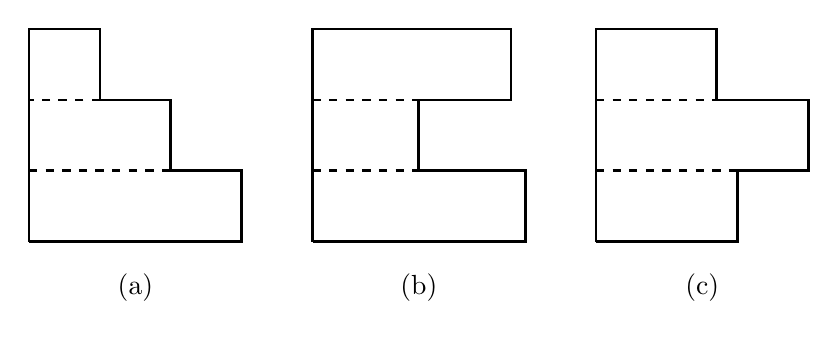
\begin{tikzpicture}[line width=1pt,scale=0.9]
\draw (-5.7,0)--(-2.7,0)--(-2.7,1.0)--(-3.7,1.0)--(-3.7,2)--(-4.7,2)--
(-4.7,3)--(-5.7,3)--(-5.7,0);
 \node[below]  at (-4.2,-0.3) {(a)};
 \draw (-1.7,0)--(1.3,0)--(1.3,1)--(-0.2,1)--(-0.2,2)--(1.1,2)--(1.1,3)--(-1.7,3)--
 (-1.7,0);
\node[below]  at (-0.2,-0.3) {(b)};
\draw (2.3,0)--(4.3,0)--(4.3,1)--(5.3,1)--(5.3,2)--(4.0,2)--
(4.0,3)--(2.3,3)--(2.3,0);
\node[below]  at (3.8,-0.3) {(c)};
\draw [dashed] (-4.7,2.0) -- (-5.7,2.0);
\draw [dashed] (-5.7,1.0) -- (-3.7,1.0);
\draw [dashed] (-1.7,2.0) -- (-0.2,2.0);
\draw [dashed] (-1.7,1.0) -- (-0.2,1.0);
\draw [dashed] (2.3,2.0) -- (4.3,2.0);
\draw [dashed] (2.3,1.0) -- (4.3,1.0);
\end{tikzpicture}
\caption{The three types of polygon corresponding to types (a),
(b) and (c). The one of type (a) is a staircase-shaped polygon.} 

\label{fig:I-1-new}
\end{figure}

The other two types can be  handled in much the same way. By applying
the $\mathbb{H}^3$-action, we can transform them into pillowcases. 
There is a correspondence between Figure  \ref{fig:I-1} and 
Figure  \ref{fig:I-1-new}.
In Type (b), we have $\ell_1 > \ell_2$ and $\ell_3>\ell_2$. 
In Type (c), we have $\ell_1 < \ell_2$ and $\ell_3< \ell_2$.  


\begin{Remark}
If $\psi$ is a pillowcase,
then the vertical foliation of $\psi$ is also Jenkins-Strebel. In other words,
  rotating $\psi$ by $\rot$ gives a new Jenkins-Strebel differential. We will show that every Jenkins-Strebel differential $\phi\in \Q(1^2, -1^6)$ can be replaced by a new $\psi$, which is a pillowcase of type (a), (b) or (c).
\end{Remark}

Next, we show that any pillowcase surface $\phi$ of type (I-1-b) or (I-1-c) can be deformed into a staircase, i.e., a Jenkins-Strebel differential of type (I-1-a). 


\subsubsection*{\textbf{(I-1-b):}} $\phi$ is of type (I-1-b). 
We can apply the $\HP^3$-action on $\phi$ using the following steps 
(as illustrated in Figure \ref{fig:I-1-b}): 



\begin{enumerate}
  \item[(i)] As a first step, we shear the cylinder $\Pi_2$ (the one in the middle)  appropriately so that the surface becomes the double of a $Z$-shaped polygon.
  \item[(ii)] Secondly, we use the $\HP^3$-action on the horizontal cylinders to adjust their heights, denoted by $h_1,h_2$ and $h_3$, to satisfy the inequality $h_1<h_2<h_3$.
      \item[(iii)] Thirdly, we apply $\rot$ to rotate the quadratic differential such that the horizontal leaves become vertical.  Then we shear the horizontal cylinder in the middle and rotate it back around so that the surface is transformed into the one in Case (I-1-a), i.e., the horizontal cylinder at the bottom has the largest circumference. 
\item[(iv)] Finally, we  
shear the horizontal cylinder in the middle  to transform the surface into a staircase.
\end{enumerate} 


\begin{figure}[h]
    \centering
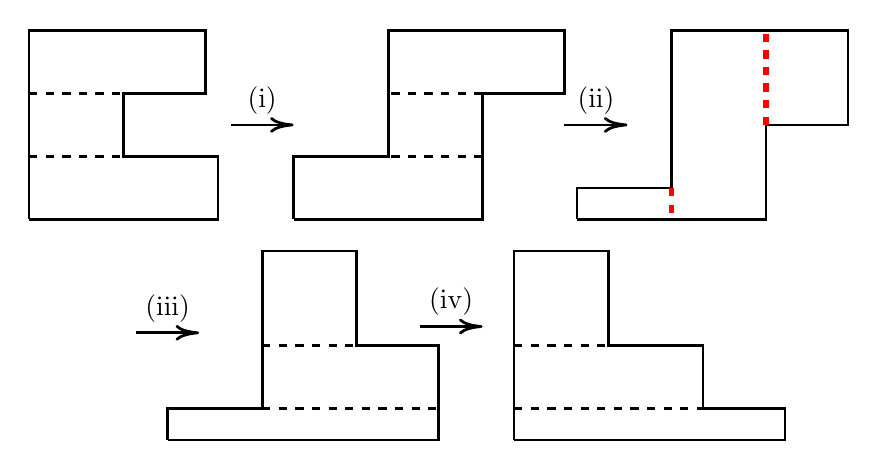
\begin{tikzpicture}[line width=1pt,scale=0.8]
%\draw (-5.7,0)--(-2.7,0)--(-2.7,1.0)--(-3.7,1.0)--(-3.7,2)--(-4.7,2)--
%(-4.7,3)--(-5.7,3)--(-5.7,0);
 %\node[below]  at (-4.2,-0.3) {(A)};
 \draw (-1.7,0)--(1.3,0)--(1.3,1)--(-0.2,1)--(-0.2,2)--(1.1,2)--(1.1,3)--(-1.7,3)--
 (-1.7,0);
\draw [dashed] (-1.7,2)--(-0.2,2);
\draw [dashed] (-1.7,1)--(-0.2,1);
\draw [dashed] (5.5,2)--(4,2);
\draw [dashed] (5.5,1)--(4,1);
 \draw [-{To[length=3mm,width=2mm]}] (1.5,1.5)--(2.5,1.5);
 \draw (2.5,0)--(5.5,0)--(5.5,2)--(6.8,2)--(6.8,3)--(4.0,3)--(4.0,1)--(2.5,1)--(2.5,0);
  \draw [-{To[length=3mm,width=2mm]}] (6.8,1.5)--(7.8,1.5);
  \draw (7.0,0)--(10.0,0)--(10.0,1.5)--(11.3,1.5)--(11.3,3)--(8.5,3)--(8.5,0.5)--(7.0,0.5)--(7.0,0);
  \draw [-{To[length=3mm,width=2mm]}] (0,-1.8)--(1,-1.8);
 \draw (0.5,-3.5)--(4.8,-3.5)--(4.8,-2)--(3.5,-2)--(3.5,-0.5)--(2,-0.5)--(2,-3)--(0.5,-3)--(0.5,-3.5);
 \draw [-{To[length=3mm,width=2mm]}] (4.5,-1.7)--(5.5,-1.7);
 \draw (6,-3.5)--(10.3,-3.5)--(10.3,-3)--(9,-3)--(9,-2)--(7.5,-2)--(7.5,-0.5)--(6,-0.5)--(6,-3.5);
\draw [color=red,line width=2pt,dashed] (10,1.5)--(10,3);
\draw [color=red,line width=2pt,dashed] (8.5,0.5)--(8.5,0);
\draw [dashed] (2,-3)--(4.8,-3);
\draw [dashed] (2,-2)--(3.5,-2);
\draw [dashed] (2,-3)--(4.8,-3);
\draw [dashed] (6,-2)--(7.5,-2);
\draw [dashed] (6,-3)--(9,-3);

\node[above]  at (2,1.5) {(i)};
\node[above]  at (7.3,1.5) {(ii)};
\node[above]  at (0.5,-1.8) {(iii)};
\node[above]  at (5,-1.7) {(iv)};

\end{tikzpicture}
\caption{The steps to deform a pillowcase surface of type (b) into a staircase. The dashed lines in color red denote vertical saddle connections.} 
\label{B-A}
\label{fig:I-1-b}
\end{figure}


%As for C-pillowcase, if the C-pillowcase in Figure \ref{fig:I-1-new}(C) has three vertical cylinders. We rotate the differential such that the horizontal leaves become vertical leaves and then shear the bottom horizontal cylinder appropriately to make it become A-pillowcase. (See the last step in Figure \ref{B-A})
%Else if it has only two vertical cylinders, we do the following steps: 
%First, we shear the second horizontal cylinder such 
%that it has three vertical cylinders.
%Second, we rotate the differential such that the horizontal cylinders become vertical cylinders.
%Third, we make $\HP^3$ acting the three horizontal cylinders such that all the height of horizontal cylinders in descending order from top to bottom.

%Then we rotate the differential such that the horizontal leaves become vertical leaves and then shear the second horizontal cylinder appropriately such that it becomes C-pillowcase with three vertical cylinders.
%Finally, rotate back and 
%shear the bottom horizontal cylinder appropriately to make it become A-pillowcase.(See Figure )

As a result, we have shown that surfaces of type  (I-1-b) can be deformed into staircases. In other words, there exists a staircase surface in the $\HP^3$-orbit of $\phi$, up to a $\rot$-rotation that changes the horizontal foliation into a vertical one. 


\subsubsection*{\textbf{(I-1-c):}} $\phi$ is of type (I-1-c). There are two possibilities.
First, if $\phi$ has three vertical cylinders, then we apply $\rot$ to rotate $\phi$ so that it becomes a surface as in the third step of the surgery that we performed for Case (I-1-b). Then we can shear the horizontal cylinder in the middle  to create a staircase.

It remains to consider the case when $\phi$ has only two vertical cylinders. This occurs when the cylinders at the top and the bottom have the same circumference. 

\begin{figure}[h]
	\centering
	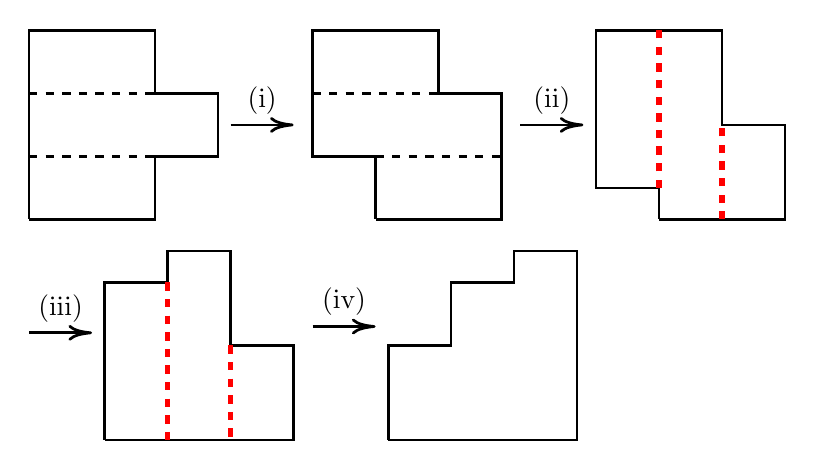
\begin{tikzpicture}[line width=1pt,scale=0.8]
		
		\draw (0,0)--(2,0)--(2,1)--(3,1)--(3,2)--(2,2)--
		(2,3)--(0,3)--(0,0);
		\draw [dashed] (0,1)--(2,1);
		\draw [dashed] (0,2)--(2,2);
		\draw [-{To[length=3mm,width=2mm]}] (3.2,1.5)--(4.2,1.5);
		\node[above]  at (3.7,1.5) {(i)};
		\draw (5.5,0)--(7.5,0)--(7.5,2)--(6.5,2)--(6.5,3)--(4.5,3)--(4.5,1)--(5.5,1)--(5.5,0);
		\draw [-{To[length=3mm,width=2mm]}] (7.8,1.5)--(8.8,1.5);
		\draw [dashed] (4.5,2)--(6.5,2);
		\draw [dashed] (5.5,1)--(7.5,1);
		\node[above]  at (8.3,1.5) {(ii)};
		\draw (10,0)--(12,0)--(12,1.5)--(11,1.5)--(11,1.5)--(11,3)--(9,3)--(9,0.5)--(10,0.5)--(10,0);
		\draw [color=red,line width=2pt,dashed] (10,0.5)--(10,3);
		\draw [color=red,line width=2pt,dashed] (11,0)--(11,1.5);
		\draw [-{To[length=3mm,width=2mm]}] (0,-1.8)--(1,-1.8);
		\node[above]  at (0.5,-1.8) {(iii)};
		\draw (1.2,-3.5)--(4.2,-3.5)--(4.2,-2)--(3.2,-2)--(3.2,-0.5)--(2.2,-0.5)--(2.2,-1)--(1.2,-1)--(1.2,-3.5);
		\draw [color=red,line width=2pt,dashed] (2.2,-1)--(2.2,-3.5);
		\draw [color=red,line width=2pt,dashed] (3.2,-2)--(3.2,-3.5);
		\draw [-{To[length=3mm,width=2mm]}] (4.5,-1.7)--(5.5,-1.7);
		\node[above]  at (5,-1.7) {(iv)}; 
		\draw (5.7,-3.5)--(8.7,-3.5)--(8.7,-0.5)--(7.7,-0.5)--(7.7,-1)--(6.7,-1)--(6.7,-2)--(5.7,-2)--(5.7,-3.5);
		%(-1.7,0);
		%\node[below]  at (-0.2,-0.3) {(B)};
		%\draw (2.3,0)--(4.3,0)--(4.3,1)--(5.3,1)--(5.3,2)--(4.0,2)--(4.0,3)--(2.3,3)--(2.3,0);
		%\node[below]  at (3.8,-0.3) {(C)};
		
	\end{tikzpicture}
	\caption{The step to deform a pillowcase of type (c) with two vertical cylinders into a staircase surface.} 
	\label{fig:I-1-c}
\end{figure}

Now, we deform $\phi$ using the following steps (as illustrated in Figure \ref{fig:I-1-c}): 



\begin{enumerate}
  \item[(i)] Note that $\phi$ has two vertical cylinders.
  By applying the $\mathbb{H}^2$-action on the vertical cylinders we can make one cylinder longer and the other one shorter. Now we examine  the horizontal cylinders. 
  We shear the horizontal cylinder in the middle appropriately so
that the new surface has three vertical cylinders. We still denote the resulting surface by $\phi$.
\item[(ii)] In the second step, we apply the $\HP^3$-action to the horizontal cylinders so that their heights strictly decrease  from top to bottom.
    \item[(iii)] Thirdly, we apply $\rot$ to rotate the quadratic differential so that the horizontal leaves become vertical. Next,
 we shear the horizontal cylinder in the middle  appropriately so that the  resulting surface becomes the one considered in the previous case. That is, the surface consists of three vertical cylinders.  
\item[(iv)] Finally, we apply $\rot$ to rotate $\phi$ to a surface as in the third step of the surgery performed for Case (I-1-b). Then we can proceed to shear the horizontal cylinder in the middle  to transform the surface into a staircase.
\end{enumerate} 



This shows that surfaces of type (I-1-c) can be deformed into staircase surfaces. 

\subsection*{Case (I-2):} Each zero of $\phi$ is connected to itself by a horizontal saddle connection, and the two zeros are joined by a horizontal saddle connection. 
This is illustrated in Figure \ref{fig:I-2}.


In this case, $\phi$ is a Jenkins-Strebel differential with three horizontal cylinders. After shearing the horizontal cylinders of $\phi$ appropriately, we obtain a quadratic differential $\psi$ in the $\mathbb{H}^3$-orbit of $\phi$, which is the double of a polygon as illustrated  in Figure \ref{fig:I-2-new}. Rotate $\psi$  by $\rot$ transforms $\psi$ into a pillowcase of type (I-1-b). 










\begin{figure}[h]
    \centering
    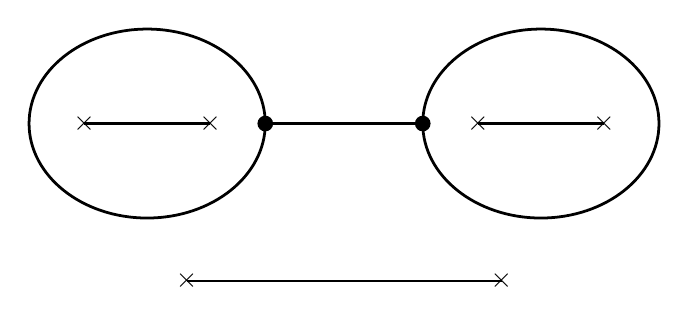
\begin{tikzpicture}[line width=1pt]
    \draw  (-2.5,0) ellipse (1.5cm and 1.2cm);
   \node[ circle, fill=black,inner sep = 2pt] (A) at (-1,0){};
    \draw  (2.5,0) ellipse (1.5cm and 1.2cm);
    \node[ circle, fill=black,inner sep = 2pt] (A) at (1,0){};
    \draw (-1,0)--(1,0);
    \draw (-3.3,0)--(-1.7,0);
    \draw (3.3,0)--(1.7,0);
    \node  at(-3.3,0){$\times$};
\node  at(3.3,0){$\times$};
\node  at(-1.7,0){$\times$};
\node  at(1.7,0){$\times$};
\draw (-2,-2.0)--(2,-2.0);
\node  at(-2,-2.0){$\times$};
\node  at(2,-2.0){$\times$};

    \end{tikzpicture}
    \caption{A Jenkins-Strebel differential in Case (I-2).}
    \label{fig:I-2}
\end{figure}




\begin{figure}[h]
    \centering
    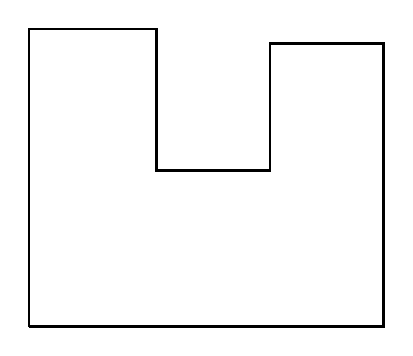
\begin{tikzpicture}[line width=1pt,scale=0.9]
     \draw (0,0)--(5,0)--(5,4)--(3.4,4)--(3.4,2.2)--(1.8,2.2)--(1.8,4.2)--(0,4.2)--(0,0);


        
    \end{tikzpicture}
    \caption{A polygon in Case (I-2).}
    \label{fig:I-2-new}
\end{figure}



\subsection*{Case \textbf{(I-3):}} 
There are three horizontal saddle connection that emanate from one zero and terminate at the other,
denoted by $\gamma_1,\gamma_2$ and $\gamma_3$, respectively. In this case, $\phi$ has three horizontal cylinders. Denote by $\widehat{p_1p_2},
\widehat{p_3p_4}$ and $\widehat{p_5p_6}$ the horizontal saddle connections joining the pairs of poles.  See Figure \ref{fig:I-6}  for an illustration.
%We denote by $\Gamma_0$ the component of $\Gamma$ that contains the zeros. 


\begin{figure}[h]
    \centering
    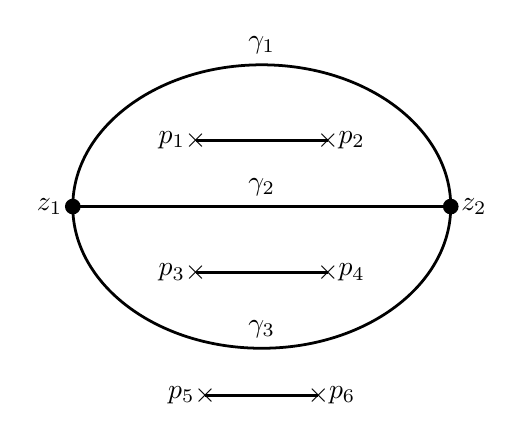
\begin{tikzpicture}[line width=1pt, scale=1.2]
        \draw (0,0) ellipse (2cm and 1.5cm);
        \draw (-2,0)--(2,0);
        \draw (-0.7,0.7)--(0.7,0.7);
        \draw (-0.7,-0.7)--(0.7,-0.7);
        \draw (-0.6,-2)--(0.6,-2);
         \node[ circle, fill=black,inner sep = 2pt] (A) at (-2,0){};
        \node[ circle, fill=black,inner sep = 2pt] (A) at (2,0){};
         \node at(-0.7,0.7){$\times$}; 
        \node  at(0.7,0.7){$\times$};
        \node at(-0.7,-0.7){$\times$}; 
       \node at(0.7,-0.7){$\times$}; 
        \node at(-0.6,-2){$\times$}; 
        \node at(0.6,-2){$\times$};
        \node[left] at(-0.7,0.7){$p_1$}; 
        \node[right]  at(0.7,0.7){$p_2$};
        \node[left] at(-0.7,-0.7){$p_3$}; 
       \node[right] at(0.7,-0.7){$p_4$}; 
        \node[left] at(-0.6,-2){$p_5$}; 
        \node[right] at(0.6,-2){$p_6$};
        \node[above] at(0,1.5){$\gamma_1$};
        \node[above] at(0,0){$\gamma_2$};
        \node[above] at(0,-1.5){$\gamma_3$};
        \node[left] at(-2,0) {$z_1$};
         \node[right] at(2,0) {$z_2$};
    \end{tikzpicture}
    \caption{Case (I-3).}
    \label{fig:I-6}
\end{figure}

With an obvious change in notation, there are three subcases as follows. 

\subsubsection*{\textbf{(I-3-a):}} Assume that $|\gamma_1|=|\gamma_2|=|\gamma_3|$.
We can  shear  the horizontal cylinders appropriately so that 
$z_1$ is connected to each of $p_1,p_3,p_5$ by a vertical saddle connection.
The assumption  $|\gamma_1|=|\gamma_2|=|\gamma_3|$ implies that 
$z_2$ is also connected to each of $p_2,p_4,p_6$ by a vertical saddle connection.
As a result, the vertical critical graph of $\phi$ consists of two trivalent trees, 
see Figure \ref{fig:I-6-1}.


\begin{figure}[h]
    \centering
    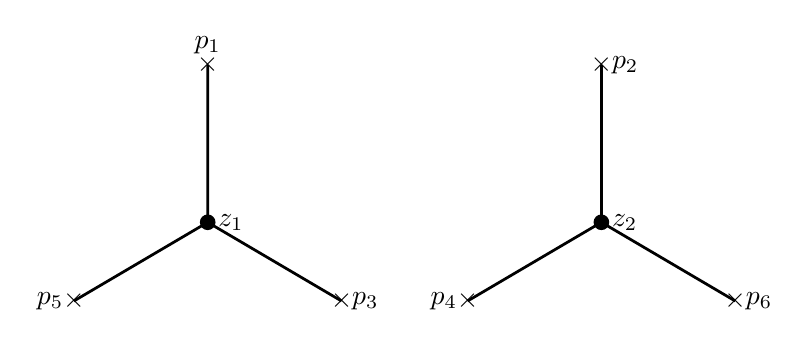
\begin{tikzpicture}[line width=1pt]
        \draw (0,0)--(0,-2)--(-1.7,-3);
        \draw (0,-2)--(1.7,-3);
        \draw (5,0)--(5,-2)--(3.3,-3);
        \draw (5,-2)--(6.7,-3);
        \node[ circle, fill=black,inner sep = 2pt] (A) at (0,-2){};
        \node[ circle, fill=black,inner sep = 2pt] (A) at (5,-2){};
         \node  at(0,0){$\times$}; 
        \node  at(1.7,-3){$\times$};
        \node  at(-1.7,-3){$\times$}; 
       \node  at(5,0){$\times$}; 
        \node  at(6.7,-3){$\times$}; 
        \node  at(3.3,-3){$\times$}; 
         \node[above] at(0,0){$p_1$}; 
        \node[right]  at(1.7,-3){$p_3$};
        \node[left] at(-1.7,-3){$p_5$}; 
       \node[right] at(5,0){$p_2$}; 
        \node[left] at(3.3,-3){$p_4$}; 
        \node[right] at(6.7,-3){$p_6$};
        \node[right] at(0,-2) {$z_1$};
         \node[right] at(5,-2) {$z_2$};
    \end{tikzpicture}
    \caption{The vertical critical graph of $\phi$ consists of two trivalent trees.}
    \label{fig:I-6-1}
\end{figure}


By applying the $\mathbb{H}^3$-action to $\phi$, we can adjust the heights of the three horizontal cylinders to be $1,2$ and $1$, respectively. 
We rotate the quadratic differential by $\rot$.
 The resulting quadratic differential, still denoted by $\phi$, 
 is a Jenkins-Strebel differential with a single cylinder that can be obtained by gluing the rectangle in Figure \ref{fig:I-6-a}.

\begin{figure}[h]
    \centering
    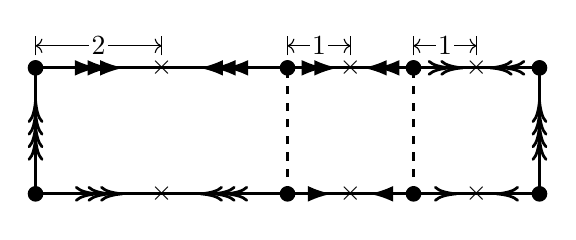
\begin{tikzpicture}[line width=1pt,scale=0.8]
        \draw (0,0) rectangle (8,2);
        \node[ circle, fill=black,inner sep = 2pt] (A) at (0,0){};
        \node[ circle, fill=black,inner sep = 2pt] (A) at (8,0){};
         \node[ circle, fill=black,inner sep = 2pt] (A) at (0,2){};
        \node[ circle, fill=black,inner sep = 2pt] (A) at (4,0){}; 
        \node[ circle, fill=black,inner sep = 2pt] (A) at (4,2){};
        \node[ circle, fill=black,inner sep = 2pt] (A) at (8,2){};
        \node[ circle, fill=black,inner sep = 2pt] (A) at (6,0){};
        \node[ circle, fill=black,inner sep = 2pt] (A) at (6,2){};
        \node at (2,0) {$\times$};
        \node at (2,2) {$\times$};
        \node at (5,0) {$\times$};
        \node at (5,2) {$\times$};
        \node at (7,0) {$\times$};
        \node at (7,2){$\times$};
        \draw [-{Latex[length=3mm,width=2mm]}]  (4,0)--(4.7,0);
        \draw (4.7,0)--(5,0);
        \draw [-{Latex[length=3mm,width=2mm]}]  (6,0)--(5.3,0);
        \draw[-{To[length=3mm,width=2mm]}]  (6,0)--(6.7,0);
         \draw[-{To[length=3mm,width=2mm]}]  (8,0)--(7.3,0);
        \draw[-{To[length=3mm,width=2mm]}]  (6,2)--(6.6,2);
         \draw[-{To[length=3mm,width=2mm]}]  (6.5,2)--(6.8,2);
         \draw[-{To[length=3mm,width=2mm]}]  (8,2)--(7.4,2);
         \draw[-{To[length=3mm,width=2mm]}]  (7.4,2)--(7.2,2);        

         
         \draw[-{Latex[length=3mm,width=2mm]}]  (4,2)--(4.6,2);
         \draw[-{Latex[length=3mm,width=2mm]}]  (4.5,2)--(4.8,2);
         \draw[-{Latex[length=3mm,width=2mm]}]  (6,2)--(5.4,2);
         \draw[-{Latex[length=3mm,width=2mm]}]  (5.4,2)--(5.2,2);        


        \draw [-{To[length=3mm,width=2mm]}] (0,0)--(1,0);
        \draw [-{To[length=3mm,width=2mm]}] (1,0)--(1.2,0);
        \draw [-{To[length=3mm,width=2mm]}] (1.2,0)--(1.4,0);
        \draw [-{To[length=3mm,width=2mm]}] (4,0)--(3,0);
        \draw [-{To[length=3mm,width=2mm]}] (3,0)--(2.8,0);
        \draw [-{To[length=3mm,width=2mm]}] (2.8,0)--(2.6,0);


        \draw [-{Latex[length=3mm,width=2mm]}] (0,2)--(1,2);
        \draw [-{Latex[length=3mm,width=2mm]}] (1,2)--(1.2,2);
        \draw [-{Latex[length=3mm,width=2mm]}] (1.2,2)--(1.4,2);
        \draw [-{Latex[length=3mm,width=2mm]}] (4,2)--(3,2);
        \draw [-{Latex[length=3mm,width=2mm]}] (3,2)--(2.8,2);
        \draw [-{Latex[length=3mm,width=2mm]}] (2.8,2)--(2.6,2);


        \draw [-{To[length=3mm,width=2mm]}] (0,0)--(0,0.9);
         \draw [-{To[length=3mm,width=2mm]}] (0,0.9)--(0,1.1); 
       \draw [-{To[length=3mm,width=2mm]}] (0,1.1)--(0,1.3);
         \draw [-{To[length=3mm,width=2mm]}] (0,1.3)--(0,1.5); 

        \draw [-{To[length=3mm,width=2mm]}] (8,0)--(8,0.9);
         \draw [-{To[length=3mm,width=2mm]}] (8,0.9)--(8,1.1); 
       \draw [-{To[length=3mm,width=2mm]}] (8,1.1)--(8,1.3);
         \draw [-{To[length=3mm,width=2mm]}] (8,1.3)--(8,1.5); 
         
         \draw [line width =0.4pt](0,2.2)--(0,2.5);
         \draw [line width =0.4pt](2,2.2)--(2,2.5);
         \draw [line width =0.4pt][->](1.15,2.35)--(2,2.35);
         \draw [line width =0.4pt][<-](0,2.35)--(0.85,2.35);  
         \node at (1,2.35) {2};

         \draw [line width =0.4pt](4,2.2)--(4,2.5);
         \draw [line width =0.4pt](5,2.2)--(5,2.5);
         \draw [line width =0.4pt][->](4.65,2.35)--(5,2.35);
         \draw [line width =0.4pt][->](4.35,2.35)--(4,2.35);  
         \node at (4.5,2.35) {1};

         \draw [line width =0.4pt](6,2.2)--(6,2.5);
         \draw [line width =0.4pt](7,2.2)--(7,2.5);
         \draw [line width =0.4pt][->](6.65,2.35)--(7,2.35);
         \draw [line width =0.4pt][->](6.35,2.35)--(6,2.35);  
         \node at (6.5,2.35) {1};
         \draw [dashed] (4,0)--(4,2);
         \draw [dashed] (6,0)--(6,2);
    \end{tikzpicture}
        \caption{The rectangle in Case (I-3-a).}
    \label{fig:I-6-a}
\end{figure}


Now we apply $\begin{pmatrix}
    1 & -2/|\gamma_i|\\
    0 & 1
\end{pmatrix}$ to shear $\phi$ (the rectangle) so that it becomes the situation illustrated in Figure \ref{fig:I-6-a2}. The new Jenkins-Strebel differential, still denoted by $\phi$,  has a pair of vertical saddle connections of equal length that connect one zero to  the other, and each zero is connected to a pole by a vertical saddle connection.  Note that the union of the pair of vertical saddle connections connecting the zeros bounds a Jordan domain containing two poles. 








\begin{figure}[h]
    \centering
    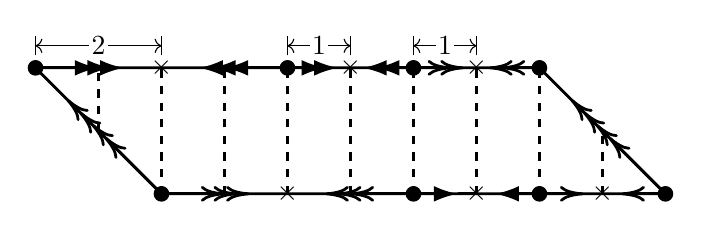
\begin{tikzpicture}[line width=1pt,scale=0.8]
        \draw (2,0)--(10,0)--(8,2)--(0,2)--(2,0);
        \node[ circle, fill=black,inner sep = 2pt] (A) at (2,0){};
        \node[ circle, fill=black,inner sep = 2pt] (A) at (10,0){};
         \node[ circle, fill=black,inner sep = 2pt] (A) at (0,2){};
        \node[ circle, fill=black,inner sep = 2pt] (A) at (6,0){}; 
        \node[ circle, fill=black,inner sep = 2pt] (A) at (4,2){};
        \node[ circle, fill=black,inner sep = 2pt] (A) at (8,2){};
        \node[ circle, fill=black,inner sep = 2pt] (A) at (8,0){};
        \node[ circle, fill=black,inner sep = 2pt] (A) at (6,2){};
        \node at (4,0) {$\times$};
        \node at (2,2) {$\times$};
        \node at (7,0) {$\times$};
        \node at (5,2) {$\times$};
        \node at (9,0) {$\times$};
        \node at (7,2){$\times$};
        \draw [-{Latex[length=3mm,width=2mm]}]  (6,0)--(6.7,0);
        \draw (6.7,0)--(7,0);
        \draw [-{Latex[length=3mm,width=2mm]}]  (8,0)--(7.3,0);
        \draw[-{To[length=3mm,width=2mm]}]  (8,0)--(8.7,0);
         \draw[-{To[length=3mm,width=2mm]}]  (10,0)--(9.3,0);
        \draw[-{To[length=3mm,width=2mm]}]  (6,2)--(6.6,2);
         \draw[-{To[length=3mm,width=2mm]}]  (6.5,2)--(6.8,2);
         \draw[-{To[length=3mm,width=2mm]}]  (8,2)--(7.4,2);
         \draw[-{To[length=3mm,width=2mm]}]  (7.4,2)--(7.2,2);        

         
         \draw[-{Latex[length=3mm,width=2mm]}]  (4,2)--(4.6,2);
         \draw[-{Latex[length=3mm,width=2mm]}]  (4.5,2)--(4.8,2);
         \draw[-{Latex[length=3mm,width=2mm]}]  (6,2)--(5.4,2);
         \draw[-{Latex[length=3mm,width=2mm]}]  (5.4,2)--(5.2,2);        


        \draw [-{To[length=3mm,width=2mm]}] (2,0)--(3,0);
        \draw [-{To[length=3mm,width=2mm]}] (3,0)--(3.2,0);
        \draw [-{To[length=3mm,width=2mm]}] (3.2,0)--(3.4,0);
        \draw [-{To[length=3mm,width=2mm]}] (6,0)--(5,0);
        \draw [-{To[length=3mm,width=2mm]}] (5,0)--(4.8,0);
        \draw [-{To[length=3mm,width=2mm]}] (4.8,0)--(4.6,0);


        \draw [-{Latex[length=3mm,width=2mm]}] (0,2)--(1,2);
        \draw [-{Latex[length=3mm,width=2mm]}] (1,2)--(1.2,2);
        \draw [-{Latex[length=3mm,width=2mm]}] (1.2,2)--(1.4,2);
        \draw [-{Latex[length=3mm,width=2mm]}] (4,2)--(3,2);
        \draw [-{Latex[length=3mm,width=2mm]}] (3,2)--(2.8,2);
        \draw [-{Latex[length=3mm,width=2mm]}] (2.8,2)--(2.6,2);


        \draw [-{To[length=3mm,width=2mm]}] (2,0)--(1.1,0.9);
         \draw [-{To[length=3mm,width=2mm]}] (1.1,0.9)--(0.9,1.1); 
       \draw [-{To[length=3mm,width=2mm]}] (0.9,1.1)--(0.7,1.3);
         \draw [-{To[length=3mm,width=2mm]}] (0.7,1.3)--(0.5,1.5); 

        \draw [-{To[length=3mm,width=2mm]}] (10,0)--(9.1,0.9);
         \draw [-{To[length=3mm,width=2mm]}] (9.1,0.9)--(8.9,1.1); 
       \draw [-{To[length=3mm,width=2mm]}] (8.9,1.1)--(8.7,1.3);
         \draw [-{To[length=3mm,width=2mm]}] (8.7,1.3)--(8.5,1.5); 
         
         \draw [line width =0.4pt](0,2.2)--(0,2.5);
         \draw [line width =0.4pt](2,2.2)--(2,2.5);
         \draw [line width =0.4pt][->](1.15,2.35)--(2,2.35);
         \draw [line width =0.4pt][<-](0,2.35)--(0.85,2.35);  
         \node at (1,2.35) {2};

         \draw [line width =0.4pt](4,2.2)--(4,2.5);
         \draw [line width =0.4pt](5,2.2)--(5,2.5);
         \draw [line width =0.4pt][->](4.65,2.35)--(5,2.35);
         \draw [line width =0.4pt][->](4.35,2.35)--(4,2.35);  
         \node at (4.5,2.35) {1};

         \draw [line width =0.4pt](6,2.2)--(6,2.5);
         \draw [line width =0.4pt](7,2.2)--(7,2.5);
         \draw [line width =0.4pt][->](6.65,2.35)--(7,2.35);
         \draw [line width =0.4pt][->](6.35,2.35)--(6,2.35);  
         \node at (6.5,2.35) {1};
         \draw [dashed] (2,0)--(2,2);
        \draw [dashed] (4,0)--(4,2);
        \draw [dashed] (6,0)--(6,2);
        \draw [dashed] (8,0)--(8,2);
         \draw [dashed] (1,1)--(1,2);
        \draw [dashed] (3,0)--(3,2);
        \draw [dashed] (5,0)--(5,2);
        \draw [dashed] (7,0)--(7,2);
        \draw [dashed] (9,0)--(9,1);
       
    \end{tikzpicture}
     \caption{Case (I-3-a) : The rectangle after the horocycle flow action. Dashed curve stands for vertical geodesic. }
    \label{fig:I-6-a2}
\end{figure}

Rotating by $\rot$, we obtain a Jenkins-Strebel differential with two horizontal cylinders 
as shown in Figure \ref{fig:I-6-0}. This case is not included in Case (I-1) or Case (I-2).
But it can be transformed into a pillowcase of type (I-1-c).
We postpone the discussion of this situation to 
Case (I-4-a). 

\begin{figure}[h]
    \centering
   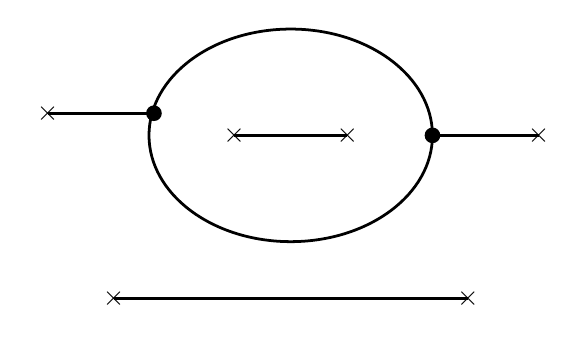
\begin{tikzpicture}[line width=1pt,scale=0.9]
    \draw (0,0) ellipse (2cm and 1.5cm);
        \node[ circle, fill=black,inner sep = 2pt] (A) at (2,0){};
        \node[ circle, fill=black,inner sep = 2pt] (A) at (-1.93,0.31225){};
       \draw (2,0)--(3.5,0);
       \draw (-1.93,0.31225)--(-3.43,0.31225);
       \node  at(3.5,0){$\times$};
       \node  at(-3.43,0.31225){$\times$};
       \draw (-0.8,0)--(0.8,0);
        \node  at(0.8,0){$\times$};
       \node  at(-0.8,0){$\times$};
       \draw (-2.5,-2.3)--(2.5,-2.3);
         \node  at(-2.5,-2.3){$\times$};
       \node  at(2.5,-2.3){$\times$};    
       %\node[left] at (-3.5,0.2){$p_1$};
      %  \node[right] at (3.5,0.2){$p_2$};
   \end{tikzpicture}
   \caption{The resulting Jenkins-Strebel differential in Case (I-3-a).}
   \label{fig:I-6-0}
\end{figure}


\subsubsection*{\textbf{(I-3-b):}} Assume that $|\gamma_1|=|\gamma_3|>|\gamma_2|$.
By  appropriately shearing the horizontal cylinders, we can assume that 
$z_1$ is connected to $p_1$ by a vertical saddle connection and $z_2$ is connected to $p_4$
by a vertical saddle connection.
Denote by $\widetilde{p_1p_2}$ the horizontal saddle connection between $p_1$ and $p_2$,
and denote  by $\widetilde{p_3p_4}$ the horizontal saddle connection between $p_3$ and $p_4$.
Note that $|\widetilde{p_3p_4}| > |\gamma_2|$. There is a vertical leaf $\delta_1$ which  emanates from $z_1$ and intersects with the interior of $\widetilde{p_3p_4}$. 
We extend the leaf until it meets with $\gamma_3$. Similarly,
there is a vertical leaf $\delta_2$ which  emanates from $z_2$ and intersects with the interior of $\widetilde{p_1p_2}$.  We extend $\delta_2$ until it meets with $\gamma_1$. 
See Figure \ref{fig:I-6-2} for an illustration. 

\begin{figure}[h!]
\centering
\includegraphics[scale=0.3]{fig6b}
    \caption{Case (I-3-b). Thick lines denote vertical saddle connections. The grey domain is a rectangle bounded by vertical and horizontal saddle connections.}
    \label{fig:I-6-2}
\end{figure}

Denote by $\widehat{z_1p_1}$ the vertical saddle connection between $z_1$ and $p_1$,
and denote by $\widehat{z_1p_4}$ the vertical saddle connection between $z_2$ and $p_4$.
As shown in Figure \ref{fig:I-6-2}, the vertical leaves $\delta_1, \widehat{z_1p_1}, \delta_2, \widehat{z_2p_4}$ together bound a vertical strip of width $|\gamma_2|$. The top and the bottom of the strip are two horizontal segments, one contained in $\gamma_1$ and the other contained in $\gamma_3$.
Let $\widetilde{p_5p_6}$ the horizontal saddle connection between $p_5$ and $p_6$. Note that 
$2 |\widetilde{p_5p_6}| = |\gamma_1| + |\gamma_3|$ and then $|\widetilde{p_5p_6}|>|\gamma_2|$. 
By  appropriately shearing the horizontal cylinder with the slit $\widetilde{p_5p_6}$, we can obtain a new surface so that the vertical strip can be enlarge to a vertical cylinder across $\widetilde{p_5p_6}$. Denote such a vertical cylinder by
$\Theta$.

Consider the new surface (still denoted by $\phi$). The complement of $\Theta$ consists of two disjoint Jordan domains. Each such domain is bounded by a vertical closed leaf passing through a zero, and the interior of each domain contains two poles. It turns out that,  in each domain, the two poles are connected by a vertical saddle connection. See Figure \ref{fig:I-3-b-2} for an illustration.
As a result, up to a rotation by $\rot$,
$\phi$ is a Jenkins-Strebel differential with three horizontal cylinders, and each zero is connected to itself by a horizontal saddle connection. Thus we can reduce this case to Case (I-1). 


\begin{figure}
    \centering
   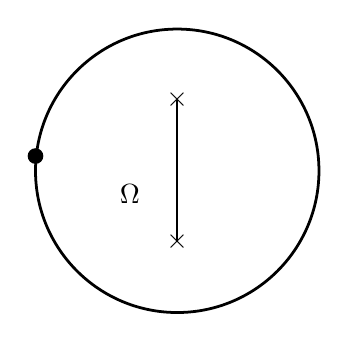
\begin{tikzpicture}[line width=1pt,scale=0.6]
    \draw (0,0) ellipse (3cm and 3cm);
        \node[ circle, fill=black,inner sep = 2pt] (A) at (-3,0.31225){};
       % \node  at(0,0){$\times$};
          \node  at(0,1.5){$\times$};
            \node  at(0,-1.5){$\times$};
   %\draw[thick] (-3,0.31225) .. controls(-2,-1) and (-1,2) .. (0,0); 
   \draw[thick] (0,1.5)-- (0,-1.5); 
   \node at(-1,-0.5){$\Omega$};
   \end{tikzpicture}
   \caption{The Jordan domain is bounded by a closed vertical saddle connection passing through a zero, with two poles in the interior.}
   \label{fig:I-3-b-2}
\end{figure}






%\begin{figure}
%    \centering
   % \includegraphics[width=0.5\linewidth]{5.8.jpg}
    %\caption{Case 6. The differential after horocycle flow. Blue dashed curve stands for vertical geodesic.}
    %\label{fig:enter-label}
%\end{figure}

\subsubsection*{\textbf{(I-3-c):}} Assume that $|\gamma_1|=|\gamma_2|<|\gamma_3|$.
Note that $|\widetilde{p_1p_2}|=|\gamma_1|=|\gamma_2|$, which is strictly less than
$|\widehat{p_3p_4}|=|\widehat{p_5p_6}|$.
By  appropriately shearing the horizontal cylinders, we can assume that there is a vertical cylinder $\Theta$ containing the interior of $\widetilde{p_1p_2}, \gamma_1$ and $\gamma_2$,
which crosses $\widetilde{p_3p_4}, \widetilde{p_5p_6}$ and $\gamma_3$. 
See Figure \ref{fig:I-6-3} for an illustration.

Now the complement of $\overline{\Theta}$ has two connected components, each of which is a Jordan domain with two poles 
in the interior. 
As a result, up to a rotation by $\rot$,
$\phi$ is a Jenkins-Strebel differential with three horizontal cylinders, and each zero is connected to itself by a horizontal saddle connection. Thus we can reduce this case to Case (I-1) again. 

\begin{figure}[h!]
\centering
\includegraphics[scale=0.3]{fig6c}
    \caption{Case (I-3-c). Thick lines denote vertical saddle connections. The grey domains are the complement of the vertical cylinder $\Theta$.}
    \label{fig:I-6-3}
\end{figure}





\subsubsection*{\textbf{(I-3-d):}} Assume that $|\gamma_2|<|\gamma_3|<|\gamma_1|$.
The proof for Case (I-3-b) applies to this case. We omit the details.

\medskip
\noindent
{\bf Jenkins-Strebel differentials with two cylinders.}

\subsection*{Case (I-4): }
The two zeros $z_1$ and $z_2$ of $\phi$ are connected by a pair of horizontal saddle connections,
and each zero is connected to a pole by a horizontal saddle connection. 
Denote by $\gamma_1$ and $\gamma_2$, respectively, the two horizontal saddle connections ending
at  $z_1$ and $z_2$. There are two horizontal saddle connections, each of which connects a pair of poles, denoted by $\alpha$ and $\beta$. 

 There are several subcases.
 
 \subsubsection*{ \textbf{(I-4-a):}}
The first subcase is illustrated in Figure \ref{fig:I-3}. We assume that 
 $|\beta|>|\alpha|$ and  $|\gamma_1| = |\gamma_2|$. The union $\gamma_1\cup\gamma_2$
bounds a Jordan domain with $\alpha$ as a slit.

Up to an $\HP^2$-action, we can assume that $p_1$
is connected to $p_5$ by a vertical saddle connection, and 
$p_3$
is connected to $z_1$ by a vertical saddle connection.
Since $|\gamma_1|=|\gamma_2|$,
  $\phi$ is the double of the polygon shown in Figure \ref{fig:I-3-1}.
Rotating $\phi$ by $\rot$, we can reduce this case to a pillowcase of type (I-1-c). 




\begin{figure}[h]
    \centering
   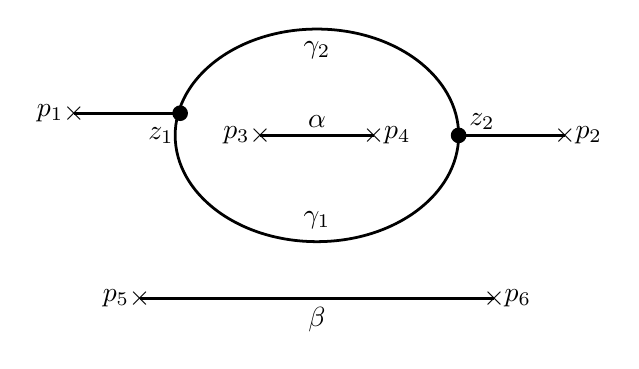
\begin{tikzpicture}[line width=1pt,scale=0.9]
    \draw (0,0) ellipse (2cm and 1.5cm);
        \node[ circle, fill=black,inner sep = 2pt] (A) at (2,0){};
        \node[ circle, fill=black,inner sep = 2pt] (A) at (-1.93,0.31225){};
       \draw (2,0)--(3.5,0);
       \draw (-1.93,0.31225)--(-3.43,0.31225);
       \node  at(3.5,0){$\times$};
       \node[right]  at(3.5,0){$p_2$};
       \node  at(-3.43,0.31225){$\times$};
       \node[left]  at(-3.43,0.31225){$p_1$};
      \node at (0,1.2) {$\gamma_2$};
       \node at (0,-1.2) {$\gamma_1$};
       \draw (-0.8,0)--(0.8,0);
        \node  at(0.8,0){$\times$};
        \node[right]  at(0.8,0){$p_4$};
       \node  at(-0.8,0){$\times$};
       \node[left]  at(-0.8,0){$p_3$};
       \draw (-2.5,-2.3)--(2.5,-2.3);
         \node  at(-2.5,-2.3){$\times$};
       \node  at(2.5,-2.3){$\times$};  
       \node[left]  at(-2.5,-2.3){$p_5$};  
      \node[right]  at(2.5,-2.3){$p_6$};  
       \node at (0,0.2) {$\alpha$};
       \node at (0,-2.6){$\beta$};
           \node at (-2.2,0){$z_1$};
       \node[right] at (2,0.2){$z_2$};
       %\node[left] at (-3.5,0.2){$p_1$};
      %  \node[right] at (3.5,0.2){$p_2$};
   \end{tikzpicture}
   \caption{Jenkins-Strebel differential in Case (I-4-a) or Case (I-4-b).}
   \label{fig:I-3}
\end{figure}


\begin{figure}[h]
    \centering
    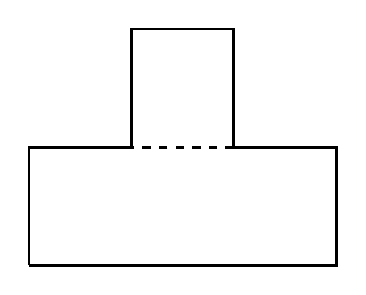
\begin{tikzpicture}[line width=1pt]
     \draw (0,0)--(3.9,0)--(3.9,1.5)--(2.6,1.5)--(2.6,3)--(1.3,3)--(1.3,1.5)--(0,1.5)--(0,0);
     \draw [dashed] (2.6,1.5)--(1.3,1.5);   
    \end{tikzpicture}
    \caption{Polygon in Case (I-4-a).}
    \label{fig:I-3-1}
\end{figure}

\subsubsection*{\textbf{(I-4-b):}}
The second subcase is the same as (I-4-a), except that 
in this case we don't have $|\gamma_1| = |\gamma_2|$. 
Without loss of generality,
we may assume that 
$|\gamma_1|>|\gamma_2|$. As before, 
up to an $\HP^2$-action, we can assume that the pole $p_1$
is connected to  $p_5$ by a vertical saddle connection, and 
$p_3$
is connected to  $z_1$ by a vertical saddle connection.


In this case, $\phi$ has two vertical cylinders, denoted by $\Theta_1$ and $\Theta_2$. See Figure \ref{fig:I-3-2} for an illustration. The first cylinder, denoted by $\Theta_1$, contains 
the interior of $\gamma_2$, and it crosses $\alpha$ and $\beta$. The second cylinder, denoted by $\Theta_2$,
is bounded by a vertical closed saddle connection passing through $z_1$ and the vertical saddle connection connecting $p_1$ to $p_5$. 



\begin{figure}[h]
\centering
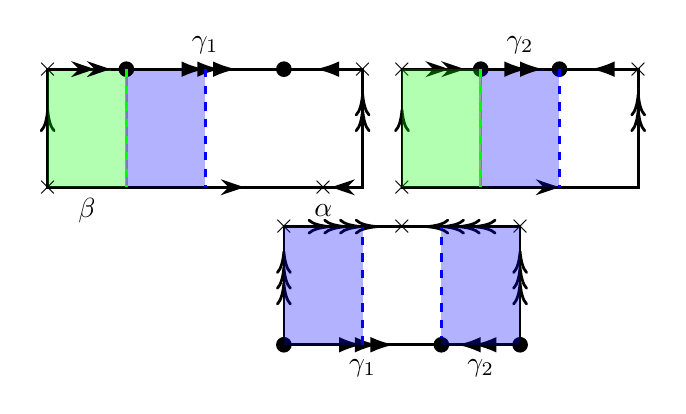
\begin{tikzpicture}[line width=1pt,scale=1]
%\draw (-4,0) rectangle (4,2);
\draw (0,0) rectangle (4,1.5);
\draw [-{Stealth[length=3mm,width=2mm]}] (0,0)--(2.5,0);
\draw(2.5,0)--(3.5,0);
\draw [-{Stealth[length=3mm,width=2mm]}] (4,0)--(3.6,0);
\draw (3.6,0)--(3.5,0);
\draw [-{To[length=3mm,width=2mm]}] (0,0)--(0,1.0);
\draw (0,1)--(0,1.5);


\draw[fill=green,opacity=0.3](1,0)--(0,0)--(0,1.5)--(1,1.5);
\draw[fill=blue,opacity=0.3](2,0)--(1,0)--(1,1.5)--(2,1.5);
%\filldraw[fill=<color>]
\draw  [-{Stealth[length=3mm,width=2mm]}](0,1.5)--(0.6,1.5);
\draw  [-{Stealth[length=3mm,width=2mm]}](0.6,1.5)--(0.8,1.5);
\draw  (0.8,1.5)--(1,1.5);
\draw  (1,1.5)--(3,1.5);
\draw [-{Latex[length=3mm,width=2mm]}]  (4,1.5)--(3.4,1.5);
\draw (3.4,1.5)--(3,1.5);
\draw [-{To[length=3mm,width=2mm]}] (4,0)--(4,1.0);
\draw [-{To[length=3mm,width=2mm]}] (4,1.0)--(4,1.2);
\draw (4,1.2)--(4,1.5);
\node (A1) at(0,0){$\times$}; 
\node(A1) at(4,1.5){$\times$};
\node (A1) at(0,1.5){$\times$}; 
\node (A1) at(3.5,0){$\times$}; 
\node[ circle, fill=black,inner sep = 2pt] (A) at (1,1.5){};
\node[ circle, fill=black,inner sep = 2pt] (A) at (3,1.5){};


\draw (4.5,0) rectangle (7.5,1.5);
\draw [-{To[length=3mm,width=2mm]}] (4.5,0)--(4.5,1);
\draw [-{To[length=3mm,width=2mm]}] (7.5,0)--(7.5,1.0);
\draw [-{To[length=3mm,width=2mm]}] (7.5,1.0)--(7.5,1.2);
\draw [-{Stealth[length=3mm,width=2mm]}] (4.5,0)--(6.5,0);
\draw  [-{Stealth[length=3mm,width=2mm]}](4.5,1.5)--(5.1,1.5);
\draw  [-{Stealth[length=3mm,width=2mm]}](5.1,1.5)--(5.3,1.5);
\draw (5.3,1.5)--(5.5,1.5);
\draw (6.5,0)--(7.5,0);
\draw (7.5,1.2)--(7.5,1.5);
\draw (4.5,1)--(4.5,1.5);

\draw [-{Latex[length=3mm,width=2mm]}]  (7.5,1.5)--(6.9,1.5);
\draw (6.9,1.5)--(6.5,1.5);
\node (A1) at(4.5,0){$\times$}; 
\node (A1) at(7.5,1.5){$\times$};
\node (A1) at(4.5,1.5){$\times$}; 
%\node [ draw,circle, inner sep = 2pt](A1) at(5.5,1.5){}; 
\node[ circle, fill=black,inner sep = 2pt] (A) at (6.5,1.5){};
\node[ circle, fill=black,inner sep = 2pt] (A) at (5.5,1.5){};


\draw [fill=green,opacity=0.3](5.5,0)--(4.5,0)--(4.5,1.5)--(5.5,1.5);
\draw [fill=blue,opacity=0.3](6.5,0)--(5.5,0)--(5.5,1.5)--(6.5,1.5);

\draw (3,-2) rectangle (6,-0.5);

\draw [-{To[length=3mm,width=2mm]}] (3,-2)--(3,-1.2);
\draw[-{To[length=3mm,width=2mm]}]  (3,-1.2)--(3,-1);
\draw[-{To[length=3mm,width=2mm]}]  (3,-1)--(3,-0.8);

%\draw [-{To[length=3mm,width=2mm]}] (3,-0.8)--(3,-0.6);
\draw (3,-0.8)--(3,-0.5);


\draw [-{To[length=3mm,width=2mm]}] (3,-0.5)--(3.6,-0.5);
\draw[-{To[length=3mm,width=2mm]}]  (3.6,-0.5)--(3.8,-0.5);
\draw[-{To[length=3mm,width=2mm]}]  (3.8,-0.5)--(4,-0.5);
\draw[-{To[length=3mm,width=2mm]}]  (4,-0.5)--(4.2,-0.5);
\draw (4.2,-0.5)--(4.5,-0.5);


\draw [-{To[length=3mm,width=2mm]}] (6,-2)--(6,-1.2);
%\draw[-{To[length=3mm,width=2mm]}]  (3,-1.2)--(3,-1);
\draw[-{To[length=3mm,width=2mm]}]  (6,-1.2)--(6,-1);

\draw [-{To[length=3mm,width=2mm]}] (6,-1)--(6,-0.8);
\draw (6,-0.8)--(6,-0.5);

\draw [-{To[length=3mm,width=2mm]}] (6,-0.5)--(5.4,-0.5);
\draw[-{To[length=3mm,width=2mm]}]  (5.4,-0.5)--(5.2,-0.5);
\draw[-{To[length=3mm,width=2mm]}]  (5.2,-0.5)--(5,-0.5);
\draw[-{To[length=3mm,width=2mm]}]  (5,-0.5)--(4.8,-0.5);
\draw (4.8,-0.5)--(4.5,-0.5);


\draw [-{Latex[length=3mm,width=2mm]}]  (5.5,1.5)--(6.1,1.5);
\draw [-{Latex[length=3mm,width=2mm]}]  (6.1,1.5)--(6.3,1.5);
\draw (6.3,1.5)--(6.5,1.5);

\draw [-{Latex[length=3mm,width=2mm]}]  (6,-2)--(5.4,-2);
\draw [-{Latex[length=3mm,width=2mm]}]  (5.4,-2)--(5.2,-2);
\draw (5.2,-2)--(5,-2);

\draw [-{Latex[length=3mm,width=2mm]}]  (1,1.5)--(2,1.5);
\draw [-{Latex[length=3mm,width=2mm]}]  (2,1.5)--(2.2,1.5);
\draw [-{Latex[length=3mm,width=2mm]}]  (2.2,1.5)--(2.4,1.5);
\draw (2.4,1.5)--(3,1.5);

\draw [-{Latex[length=3mm,width=2mm]}]  (3,-2)--(4,-2);
\draw [-{Latex[length=3mm,width=2mm]}]  (4,-2)--(4.2,-2);
\draw [-{Latex[length=3mm,width=2mm]}]  (4.2,-2)--(4.4,-2);
\draw (4.4,-2)--(5,-2);



\draw[dashed,green](1,1.5)--(1,0);
\draw[dashed,green](5.5,1.5)--(5.5,0);
\draw[dashed,blue](2,1.5)--(2,0);
\draw[dashed,blue](6.5,1.5)--(6.5,0);
\draw[dashed,blue](4,-2)--(4,-0.5);
\draw[dashed,blue](5,-2)--(5,-0.5);


\node[ circle, fill=black,inner sep = 2pt] (A) at (3,-2){};
\node[ circle, fill=black,inner sep = 2pt] (A) at (6,-2){};
\node[ circle, fill=black,inner sep = 2pt] (A) at (5,-2){};
\node (A1) at(3,-0.5){$\times$}; 
\node (A1) at(4.5,-0.5){$\times$};
\node (A1) at(6,-0.5){$\times$};
\node at (2,1.8) {$\gamma_1$};
\node at (6,1.8) {$\gamma_2$};
\node at (4,-2.3) {$\gamma_1$};
\node at (5.5,-2.3) {$\gamma_2$};
\node[above] at (3.5,-0.5) {$\alpha$};
\node[below] at (0.5,0) {$\beta$};
\draw[fill=blue,opacity=0.3](4,-2)--(3,-2)--(3,-0.5)--(4,-0.5);
\draw[fill=blue,opacity=0.3](5,-2)--(6,-2)--(6,-0.5)--(5,-0.5);
\end{tikzpicture}
    \caption{Case (I-4-b): The surface is obtained by gluing the three rectangles 
    along the sizes with the same arrow. The green shadow domain stands for the first vertical cylinder and the blue shadow domain stands for the second vertical cylinder.}
    \label{fig:enter-label}
    \label{fig:I-3-2}
\end{figure}


Note that the complement of $\overline{\Theta_1}\cup\overline{\Theta_2}$ is a Jordan domain
$\Omega$, which contains three poles in the interior. The boundary $\partial\Omega$
is a closed vertical saddle connection passing through $z_2$. There is a unique vertical critical leaf called $\delta$ emanating from $z_2$.  See Figure \ref{fig:I-4-0} for an illustration.

\begin{figure}
    \centering
   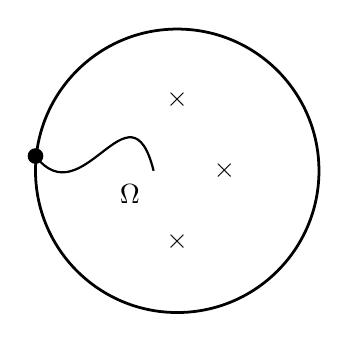
\begin{tikzpicture}[line width=1pt,scale=0.6]
    \draw (0,0) ellipse (3cm and 3cm);
        \node[ circle, fill=black,inner sep = 2pt] (A) at (-3,0.31225){};
        \node  at(1,0){$\times$};
          \node  at(0,1.5){$\times$};
            \node  at(0,-1.5){$\times$};
   \draw[thick] (-3,0.31225) .. controls(-2,-1) and (-1,2) .. (-0.5,0); 
   \node at(-1,-0.5){$\Omega$};
   \end{tikzpicture}
   \caption{The Jordan domain is bounded by a closed vertical saddle connection passing through $z_2$.}
   \label{fig:I-4-0}
\end{figure}

 If $\delta$ terminates at a pole, then the vertical foliation of $\phi$ is Jenkins-Strebel. In this case,  we can reduce $\phi$ to Case (I-1) using the  $\rot$-action. If $\delta$ does not terminate at a pole, then it is minimal in $\Omega$ (This case is similar to a minimal foliation in a four-punctured sphere). Replace $\phi$ by $\rot \cdot \phi$.
 By Theorem \ref{thm:SW},   there
is a new Jenkins-Strebel differential $\psi$ in $\overline{H\cdot \phi}$ which has at least three horizontal cylinders. Since any Jenkins-Strebel differential on $S_{0,6}$ has at most three cylinders, $\psi$ has exactly three horizontal cylinders. Thus we can reduce $\phi$ to the case of Jenkins-Strebel differential with three cylinders.





\subsubsection*{\textbf{(I-4-c):}} 
The third subcase is illustrated in Figure \ref{fig:I-3-c}, where
the union $\gamma_1\cup\gamma_2$
separates the surface into two components, each containing three poles. We assume that $|\gamma_1|=|\gamma_2|$. 

Up to an $\HP^2$-action, we can assume $p_5$
is connected to $p_1$ by a vertical saddle connection, and 
 $p_3$
is connected to  $z_1$ by a vertical saddle connection.
In this case $\phi$ is the double of the polygon 
 illustrated in Figure \ref{fig:I-3-c(P)}.
Rotate  $\phi$ by $\rot$. 
Then the resulting Jenkins-Strebel differential has three horizontal cylinders, with each zero connected to itself by a horizontal saddle connection. This is exactly the one described in Case (I-1-c). 



\begin{figure}[h]
    \centering
   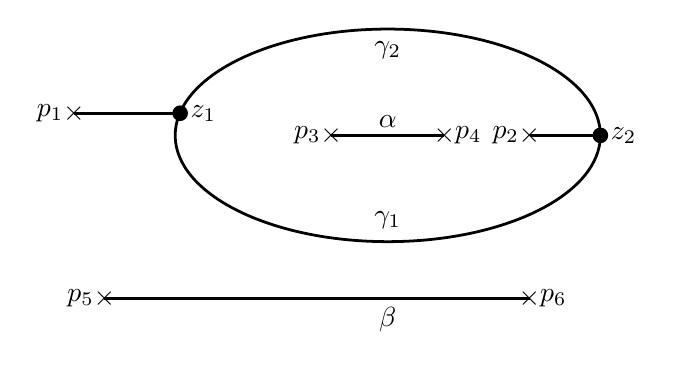
\begin{tikzpicture}[line width=1pt,scale=0.9]
    \draw (0,0) ellipse (3cm and 1.5cm);
        \node[ circle, fill=black,inner sep = 2pt] (A) at (3,0){};
        \node[ circle, fill=black,inner sep = 2pt] (A) at (-2.93,0.31225){};
       \draw (3,0)--(2,0);
       \draw (-2.93,0.31225)--(-4.43,0.31225);
       \node  at(2,0){$\times$};
       \node  at(-4.43,0.31225){$\times$};
       \node[left]  at(-4.43,0.31225){$p_1$};
        \node[left]  at(2,0){$p_2$};
      \node at (0,1.2) {$\gamma_2$};
       \node at (0,-1.2) {$\gamma_1$};
       \draw (-0.8,0)--(0.8,0);
        \node  at(0.8,0){$\times$};
       \node  at(-0.8,0){$\times$};
        \node[right]  at(0.8,0){$p_4$};
       \node[left]  at(-0.8,0){$p_3$};
       \draw (-4,-2.3)--(2,-2.3);
         \node  at(-4,-2.3){$\times$};
       \node  at(2,-2.3){$\times$};   
         \node[left]  at(-4,-2.3){$p_5$};
       \node[right]  at(2,-2.3){$p_6$};   
       \node at (0,0.2) {$\alpha$};
       \node at (0,-2.6){$\beta$};
        \node[right] at (3,0) {$z_2$};
          \node[right] at (-2.93,0.31225) {$z_1$}; 
       %\node at (-2.2,-0.7){$\Gamma_0$};
   \end{tikzpicture}
   \caption{Case (I-4-c).}
   \label{fig:I-3-c}
\end{figure}






\begin{figure}[h]
    \centering
    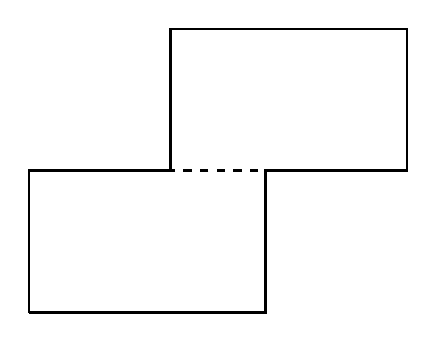
\begin{tikzpicture}[line width=1pt,scale=1.2]
     \draw (0,0)--(2.5,0)--(2.5,1.5)--(4,1.5)--(4,3)--(1.5,3)--(1.5,1.5)--(0,1.5)--(0,0);
     \draw [dashed] (2.6,1.5)--(1.3,1.5);


        
    \end{tikzpicture}
    \caption{Polygon in Case (I-4-c).}
     \label{fig:I-3-c(P)}
\end{figure}







%\begin{figure}
    %\centering
    %\includegraphics[width=0.5\linewidth]{7.jpg}
    %\caption{Polygon of Case 3 subcase 1}
    %\label{fig:enter-label}
%\end{figure}




\subsubsection*{\textbf{(I-4-d):}} 
The remaining subcase is the same as (I-4-c), except that we don't have 
 $|\gamma_1|=|\gamma_2|$. 
Without loss of generality, we may assume that $|\gamma_1| > |\gamma_2|$.
We can shear the horizontal cylinders appropriately to transform $\phi$ into the one as shown in Figure \ref{fig:I-3-d}. There are two vertical cylinders $\Theta_1$ and $\Theta_2$ such that the complement of  $\overline{\Theta_1}\cup\overline{ \Theta_2}$ is a Jordan domain containing 
three poles. Replace $\phi$ by $\rot \cdot \phi$. 
Similar to our discussion in Case (I-4-b), either $\phi$ has three or two horizontal cylinders.  
In the later case, we can apply Theorem \ref{thm:SW} to produce a new Jenkins-Strebel differential $\psi$ with three horizontal cylinders. 

\begin{figure}[h]
\centering
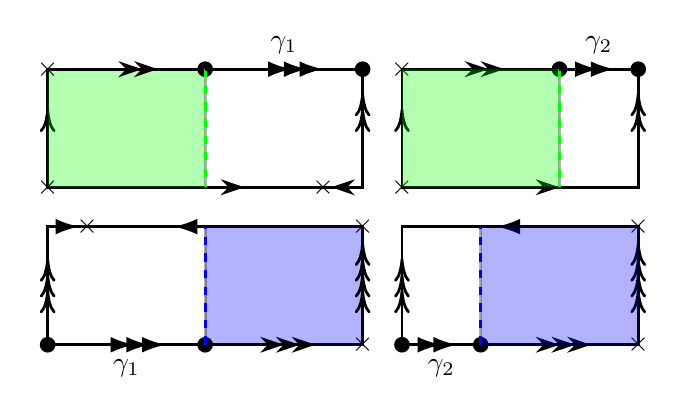
\begin{tikzpicture}[line width=1pt]
%\draw (-4,0) rectangle (4,2);
\draw (0,0) rectangle (4,1.5);
\draw [-{Stealth[length=3mm,width=2mm]}] (0,0)--(2.5,0);
\draw(2.5,0)--(3.5,0);
\draw [-{Stealth[length=3mm,width=2mm]}] (4,0)--(3.6,0);
\draw (3.6,0)--(3.5,0);
\draw [-{To[length=3mm,width=2mm]}] (0,0)--(0,1.0);
\draw (0,1)--(0,1.5);


\draw[fill=green,opacity=0.3](2,0)--(0,0)--(0,1.5)--(2,1.5)--(2,0);
%\draw[fill=blue,opacity=0.3](2,0)--(1,0)--(1,1.5)--(2,1.5);
%\filldraw[fill=<color>]
\draw  [-{Stealth[length=3mm,width=2mm]}](0,1.5)--(1.2,1.5);
\draw  [-{Stealth[length=3mm,width=2mm]}](1.2,1.5)--(1.4,1.5);
\draw  (1.4,1.5)--(2,1.5);
\draw  (1,1.5)--(3,1.5);
%\draw [-{Latex[length=3mm,width=2mm]}]  (4,1.5)--(3.4,1.5);
\draw (3.4,1.5)--(3,1.5);
\draw [-{To[length=3mm,width=2mm]}] (4,0)--(4,1.0);
\draw [-{To[length=3mm,width=2mm]}] (4,1.0)--(4,1.2);
\draw (4,1.2)--(4,1.5);
\node (A1) at(0,0){$\times$}; 
\node[ circle, fill=black,inner sep = 2pt] (A) at (4,1.5){};
\node (A1) at(0,1.5){$\times$}; 
\node (A1) at(3.5,0){$\times$}; 
%\node[ circle, fill=black,inner sep = 2pt] (A) at (1,1.5){};
\node[ circle, fill=black,inner sep = 2pt] (A) at (2,1.5){};


\draw (4.5,0) rectangle (7.5,1.5);
\draw [-{To[length=3mm,width=2mm]}] (4.5,0)--(4.5,1);
\draw [-{To[length=3mm,width=2mm]}] (7.5,0)--(7.5,1.0);
\draw [-{To[length=3mm,width=2mm]}] (7.5,1.0)--(7.5,1.2);
\draw [-{Stealth[length=3mm,width=2mm]}] (4.5,0)--(6.5,0);
\draw  [-{Stealth[length=3mm,width=2mm]}](4.5,1.5)--(5.6,1.5);
\draw  [-{Stealth[length=3mm,width=2mm]}](5.6,1.5)--(5.8,1.5);
\draw (5.8,1.5)--(6.5,1.5);
\draw (6.5,0)--(7.5,0);
\draw (7.5,1.2)--(7.5,1.5);
\draw (4.5,1)--(4.5,1.5);

%\draw [-{Latex[length=3mm,width=2mm]}]  (7.5,1.5)--(6.9,1.5);
\draw (6.9,1.5)--(6.5,1.5);
\node (A1) at(4.5,0){$\times$}; 
%\node (A1) at(7.5,1.5){$\times$};
\node (A1) at(4.5,1.5){$\times$}; 
%\node [ draw,circle, inner sep = 2pt](A1) at(5.5,1.5){}; 
\node[ circle, fill=black,inner sep = 2pt] (A) at (6.5,1.5){};
%\node[ circle, fill=black,inner sep = 2pt] (A) at (5.5,1.5){};

\node[ circle, fill=black,inner sep = 2pt] (A) at (7.5,1.5){};
\draw [fill=green,opacity=0.3](6.5,0)--(4.5,0)--(4.5,1.5)--(6.5,1.5)--(6.5,0);
%\draw [fill=blue,opacity=0.3](6.5,0)--(5.5,0)--(5.5,1.5)--(6.5,1.5);



%\draw[dashed,green](1,1.5)--(1,0);
%\draw[dashed,green](5.5,1.5)--(5.5,0);
\draw[dashed,green](2,1.5)--(2,0);
\draw[dashed,green](6.5,1.5)--(6.5,0);
%\draw[dashed,blue](4,-2)--(4,-0.5);
%\draw[dashed,blue](5,-2)--(5,-0.5);

\node at (3,1.8) {$\gamma_1$};
\node at (7,1.8) {$\gamma_2$};


\draw [-{Latex[length=3mm,width=2mm]}]  (6.5,1.5)--(7.0,1.5);
\draw [-{Latex[length=3mm,width=2mm]}]  (7.0,1.5)--(7.2,1.5);
%\draw [-{Latex[length=3mm,width=2mm]}]  (2,1.5)--(2.2,1.5);
%\draw [-{Latex[length=3mm,width=2mm]}]  (2.2,1.5)--(2.4,1.5);

\draw [-{Latex[length=3mm,width=2mm]}]  (2,1.5)--(3.1,1.5);
\draw [-{Latex[length=3mm,width=2mm]}]  (3.1,1.5)--(3.3,1.5);
\draw [-{Latex[length=3mm,width=2mm]}]  (3.3,1.5)--(3.5,1.5);



\draw (0,-2) rectangle (4,-0.5);


%\draw [-{Stealth[length=3mm,width=2mm]}] (0,-0.5)--(2.5,0);
%\draw(2.5,0)--(3.5,0);
%\draw [-{Stealth[length=3mm,width=2mm]}] (4,0)--(3.6,0);
%\draw (3.6,0)--(3.5,0);

%\draw (0,1)--(0,1.5);
\draw [-{Latex[length=3mm,width=2mm]}]  (0,-2)--(1.1,-2);
\draw [-{Latex[length=3mm,width=2mm]}]  (1.1,-2)--(1.3,-2);
\draw [-{Latex[length=3mm,width=2mm]}]  (1.3,-2)--(1.5,-2);

\draw [-{Latex[length=3mm,width=2mm]}]  (0,-0.5)--(0.4,-0.5);
\draw [-{Latex[length=3mm,width=2mm]}]  (4,-0.5)--(1.6,-0.5);


\draw[fill=blue,opacity=0.3](2,-2)--(2,-0.5)--(4,-0.5)--(4,-2)--(2,-2);
%\draw[fill=blue,opacity=0.3](2,0)--(1,0)--(1,1.5)--(2,1.5);
%\filldraw[fill=<color>]




\draw  [-{Stealth[length=3mm,width=2mm]}](2,-2)--(3,-2);
\draw  [-{Stealth[length=3mm,width=2mm]}](3,-2)--(3.2,-2);
\draw  [-{Stealth[length=3mm,width=2mm]}](3.2,-2)--(3.4,-2);
%\draw  (1.4,1.5)--(2,1.5);
%\draw  (1,1.5)--(3,1.5);
%\draw [-{Latex[length=3mm,width=2mm]}]  (4,1.5)--(3.4,1.5);

%\draw (3.4,1.5)--(3,1.5);
\draw [-{To[length=3mm,width=2mm]}] (0,-2)--(0,-1.3);
\draw [-{To[length=3mm,width=2mm]}] (0,-1.3)--(0,-1.1);
\draw [-{To[length=3mm,width=2mm]}] (0,-1.1)--(0,-0.9);

%\draw (4,1.2)--(4,1.5);
%\node (A1) at(0,-0.5){$\times$}; 
\node(A1) at(4,-2){$\times$};
\node (A1) at(0.5,-0.5){$\times$}; 
\node (A1) at(4,-0.5){$\times$}; 
\node[ circle, fill=black,inner sep = 2pt] (A) at (0,-2){};
\node[ circle, fill=black,inner sep = 2pt] (A) at (2,-2){};
\draw [-{To[length=3mm,width=2mm]}] (4,-2)--(4,-1.3);
\draw [-{To[length=3mm,width=2mm]}] (4,-1.3)--(4,-1.1);
\draw [-{To[length=3mm,width=2mm]}] (4,-1.1)--(4,-0.9);

\draw [-{To[length=3mm,width=2mm]}] (4,-0.9)--(4,-0.7);








\draw (4.5,-2) rectangle (7.5,-0.5);
\draw [-{To[length=3mm,width=2mm]}] (4.5,-2)--(4.5,-1.3);
\draw [-{To[length=3mm,width=2mm]}] (4.5,-1.3)--(4.5,-1.1);
\draw [-{To[length=3mm,width=2mm]}] (4.5,-1.1)--(4.5,-0.9);


\draw [-{To[length=3mm,width=2mm]}] (7.5,-2)--(7.5,-1.3);
\draw [-{To[length=3mm,width=2mm]}] (7.5,-1.3)--(7.5,-1.1);
\draw [-{To[length=3mm,width=2mm]}] (7.5,-1.1)--(7.5,-0.9);

\draw [-{To[length=3mm,width=2mm]}] (7.5,-0.9)--(7.5,-0.7);



\draw [-{Latex[length=3mm,width=2mm]}] (7.5,-0.5)--(5.7,-0.5);
\draw  [-{Latex[length=3mm,width=2mm]}](4.5,-2)--(5,-2);
\draw  [-{Latex[length=3mm,width=2mm]}](5,-2)--(5.2,-2);

\draw  [-{Stealth[length=3mm,width=2mm]}](5.5,-2)--(6.5,-2);
\draw  [-{Stealth[length=3mm,width=2mm]}](6.5,-2)--(6.7,-2);
\draw  [-{Stealth[length=3mm,width=2mm]}](6.7,-2)--(6.9,-2);


%\draw [-{Latex[length=3mm,width=2mm]}]  (7.5,1.5)--(6.9,1.5);

\node (A1) at(7.5,-2){$\times$}; 
%\node (A1) at(7.5,1.5){$\times$};
\node (A1) at(7.5,-0.5){$\times$}; 
%\node [ draw,circle, inner sep = 2pt](A1) at(5.5,1.5){}; 
\node[ circle, fill=black,inner sep = 2pt] (A) at (4.5,-2){};
%\node[ circle, fill=black,inner sep = 2pt] (A) at (5.5,1.5){};

\node[ circle, fill=black,inner sep = 2pt] (A) at (5.5,-2){};
\draw [fill=blue,opacity=0.3](7.5,-2)--(5.5,-2)--(5.5,-0.5)--(7.5,-0.5)--(7.5,-2);
%\draw [fill=blue,opacity=0.3](6.5,0)--(5.5,0)--(5.5,1.5)--(6.5,1.5);



%\draw[dashed,green](1,1.5)--(1,0);
%\draw[dashed,green](5.5,1.5)--(5.5,0);
\draw[dashed,blue](2,-2)--(2,-0.5);
\draw[dashed,blue](5.5,-2)--(5.5,-0.5);
%\draw[dashed,blue](4,-2)--(4,-0.5);
%\draw[dashed,blue](5,-2)--(5,-0.5);

\node at (1,-2.3) {$\gamma_1$};
\node at (5,-2.3) {$\gamma_2$};



%\draw[fill=blue,opacity=0.3](4,-2)--(3,-2)--(3,-0.5)--(4,-0.5);
%\draw[fill=blue,opacity=0.3](5,-2)--(6,-2)--(6,-0.5)--(5,-0.5);
\end{tikzpicture}
    \caption{Case (I-4-d) : The green shadow domain stands for the first vertical cylinder and the blue shadow domain stands for the second vertical cylinder.}
    \label{fig:I-3-d}
\end{figure}






%\begin{figure}
   % \centering
    %\includegraphics[width=0.6\linewidth]{5.2.jpg}
    %\caption{Crosses indicate poles, and the large dot indicates a zero. The green shadow domain stands for the first vertical cylinder and the blue shadow domain stands for the second vertical cylinder.}
    %\label{fig:enter-label}
%\end{figure}




 
\subsection*{Case \textbf{(I-5):}} The two zeros of $\phi$ are connected by a unique horizontal saddle connection, and one of the zeros is connected  to itself by a horizontal saddle connection, see Figure \ref{fig:I-5}.


\begin{figure}[h]
    \centering
    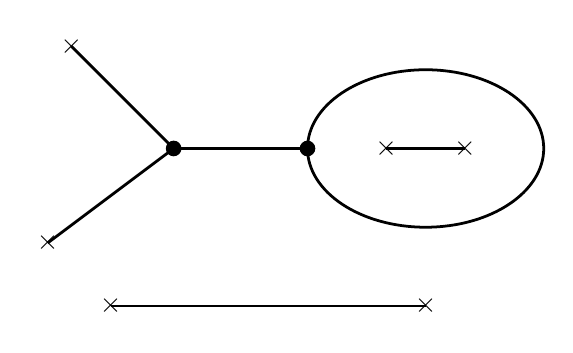
\begin{tikzpicture}[line width=1pt]
        \draw (0,0)--(1.3,-1.3)--(3,-1.3);
        \draw (-0.3, -2.5)--(1.3,-1.3);
        \draw (4.5,-1.3) ellipse (1.5cm and 1 cm);
        \draw (4.0,-1.3)--(5,-1.3);
        \draw (0.5,-3.3)--(4.5,-3.3);
         \node[ circle, fill=black,inner sep = 2pt] (A) at (1.3,-1.3){};
        \node[ circle, fill=black,inner sep = 2pt] (A) at (3,-1.3){};
                \node at(0,0){$\times$}; 
        \node  at(-0.3, -2.5){$\times$};
\node at(4.0,-1.3){$\times$}; 
\node  at(5,-1.3){$\times$}; 
\node  at(0.5,-3.3){$\times$}; 
        \node  at(4.5,-3.3){$\times$};
    \end{tikzpicture}
    \caption{Case (I-5).}
    \label{fig:I-5}
\end{figure}

 
 By  appropriately shearing the horizontal cylinders, we can assume that each zero
  is connected  to itself by a vertical saddle connection. These two vertical saddle connections bounds a cylinder, whose complement is two disjoint Jordan domains. Each such Jordan domain contains three poles in its interior. 
  
  Rotating  $\phi$ by $\rot$,
   the resulting quadratic differential (still denoted by $\phi$) may be Jenkins-Strebel or not.
     If it is Jenkins-Strebel, then it must have three horizontal cylinders. Then we can reduce $\phi$
     to Case (I-1). 
      If it is not Jenkins-Strebel, then we apply Theorem \ref{thm:SW} to produce a new Jenkins-Strebel differential $\psi$ in $\overline{H\cdot \phi}$ with three horizontal cylinders. 





\subsection*{Case \textbf{(I-6):}} In this case,
one of the zeros say $z_1$ is connected to itself by a horizontal saddle connection, 
denoted by $\beta$. The other zero $z_2$ is connected to three poles by horizontal saddle connections.



\begin{figure}[h]
    \centering
    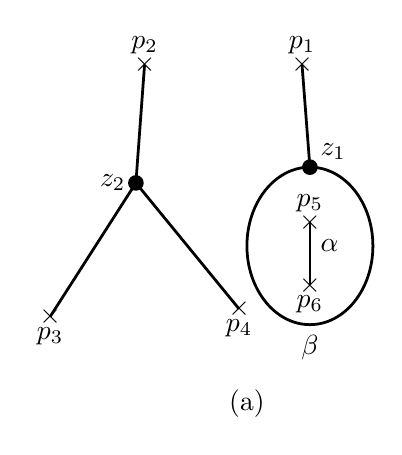
\begin{tikzpicture}[line width=1pt,scale=1]
        \draw (0,0)--(-0.11,-1.5)--(-1.2,-3.2);
        \draw (-0.11,-1.5)--(1.2,-3.1);
        \draw (2.1,-2.3) ellipse (0.8cm and 1.0cm);
        \draw (2.1,-1.3)--(2.0,0);
        \draw (2.1,-2)--(2.1,-2.8);
         \node[ circle, fill=black,inner sep = 2pt] (A) at (-0.11,-1.5){};
        \node[ circle, fill=black,inner sep = 2pt] (A) at (2.1,-1.3){};
         \node at(0,0){$\times$}; 
        \node  at(-1.2,-3.2){$\times$};
        \node  at(1.2,-3.1){$\times$}; 
       \node  at(2.0,0){$\times$}; 
        \node  at(2.1,-2){$\times$}; 
        \node  at(2.1,-2.8){$\times$}; 
        \node at (1.3,-4.3) {(a)};

        \node[left] at (-0.11,-1.5) {$z_2$};
        \node[right] at (2.1,-1.1) {$z_1$};
         \node[above] at(0,0){$p_2$};
         \node[above] at(2,0){$p_1$};
           \node[above] at(2.1,-2){$p_5$};
             \node[below] at(2.1,-2.8){$p_6$};
         \node[below] at(-1.2,-3.2){$p_3$};
         \node[below] at(1.2,-3.1){$p_4$};
            \node[below] at(2.1,-3.3){$\beta$};
      \node[right] at(2.1,-2.3){$\alpha$};
    \end{tikzpicture}

\caption{Case (I-6-a). }
       \label{fig:I-7-1} 
\end{figure}




\subsubsection*{\textbf{(I-6-a):}} See Figure \ref{fig:I-7-1} for an illustration. 
Denote by $\gamma_1$ the horizontal saddle connections connecting $z_1$ 
to $p_1$. 
Denote by $\gamma_i$ the horizontal saddle connection connecting $z_2$ to $p_i$ 
by $\gamma_i$, where $i=2,3,4$. 
Without loss of generality, we may assume that 
$|\gamma_2| = \max\{ |\gamma_2|, |\gamma_3|, |\gamma_4|\}.$
Denote by $\alpha$ the horizontal saddle connections connecting $p_5$ 
to $p_6$. 
We have the equation
\begin{equation}\label{equ:length}
  |\gamma_2|+|\gamma_3|+|\gamma_4| = |\gamma_1| + |\alpha|.
\end{equation}

There are several subcases. 





We first consider the subcase that $|\gamma_1|< |\gamma_2|$. 
By  appropriately shearing the two horizontal cylinders, we may assume that $z_1$ is connected to
$p_5$ by a vertical saddle connection, and $p_1$ is connected to $p_2$ by a vertical saddle connection. Denote the above vertical saddle connections by $\widehat{z_1p_5}$ and $\widehat{p_1p_2}$, respectively. 




There is a vertical cylinder with leaves surrounding
$\widehat{p_1p_2}$, denoted by $\Theta_1$. Since $|\gamma_1|<|\gamma_2|$, 
$\Theta_1$ must be bounded by a vertical closed saddle connection through $z_1$.  

 Now, we examine the vertical leaves near the boundary of $\overline{\Theta_1}$. Any vertical leaf  sufficiently close 
 to $\partial\overline{\Theta_1}$ travels along $\partial\overline{\Theta_1}$, and when it gets close to $z_1$,
 it turns right (or left) and follows the direction of $\widehat{z_1p_5}$ until it is close to $p_5$. Then it turns around
 and returns to $z_1$. If it keeps going, it will return to the starting point.
 
 We conclude that there is a vertical cylinder $\Theta_2$ adjoint to $\Theta_1$. Since $|\gamma_2|-|\gamma_1|< |\alpha|$, the zero $z_2$ must lie on the boundary of $\Theta_2$.  This is illustrated in Figure \ref{fig:I-7-a}.
 The complement of $\overline{\Theta_1}\cup \overline{\Theta_2}$, denoted by $\Omega$,  is a Jordan domain containing three poles.
Therefore, either $\Omega$ corresponds to the third vertical cylinder $\Theta_3$ or the vertical leaf in $\Omega$ emanating from $z_2$ is minimal. 
Replace $\phi$ by $\rot \cdot \phi$. 
In the later case, we apply Theorem \ref{thm:SW} to produce a new Jenkins-Strebel differential $\psi$ in $\overline{H\cdot \phi}$ with three horizontal cylinders. 


\begin{figure}[h]
    \centering
    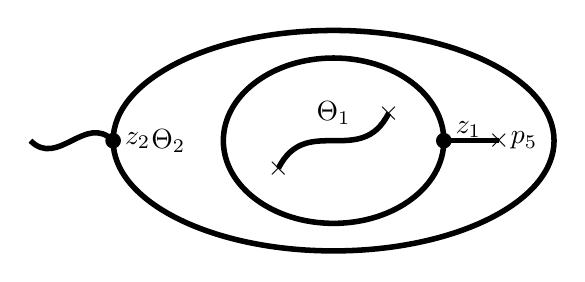
\begin{tikzpicture}[line width=2pt,scale=0.7]
    \draw (0,0) ellipse (2cm and 1.5cm);
        \node[ circle, fill=black,inner sep = 2pt] (A) at (2,0){};
        \node at (-1,-0.5) {$\times$}; 
        \node at (1,0.5) {$\times$}; 
        \draw (-1,-0.5).. controls (-0.5,0.5) and (0.5,-0.5) .. (1,0.5);
        \draw (2,0) -- (3,0);
         \draw (0,0) ellipse (4cm and 2cm);
        \node at (3,0) {$\times$}; 
        \node at (0,0.5) {$\Theta_1$};
            \node at (-3,0) {$\Theta_2$};
             \node[right] at (2,0.2) {$z_1$};
    \node[right] at (3,0) {$p_5$};
       \node[ circle, fill=black,inner sep = 2pt] (A) at (-4,0){};
        \node[right] at (-4,0) {$z_2$};
        \draw (-4,0) .. controls (-4.5,0.5) and (-5,-0.5) .. (-5.5,0);
    \end{tikzpicture}
\caption{Case (I-6-a): The  vertical cylinders  $\Theta_1$ and $\Theta_2$. }
       \label{fig:I-7-a} 
\end{figure}


Next, we consider the subcase that $|\gamma_1|= |\gamma_2|$. We can  appropriately shearing the horizontal cylinders so that $p_1$ is connected to
$p_2$ by a vertical saddle connection.
Now we shear the horizontal cylinder bounded by $\alpha$ and $\beta$ so that $p_4$ is connected to
$p_6$ by a vertical saddle connection. Denote the above vertical saddle connections by $\widehat{p_1p_2}$ and $\widehat{p_4p_6}$, respectively. 



\begin{figure}[h]
    \centering
    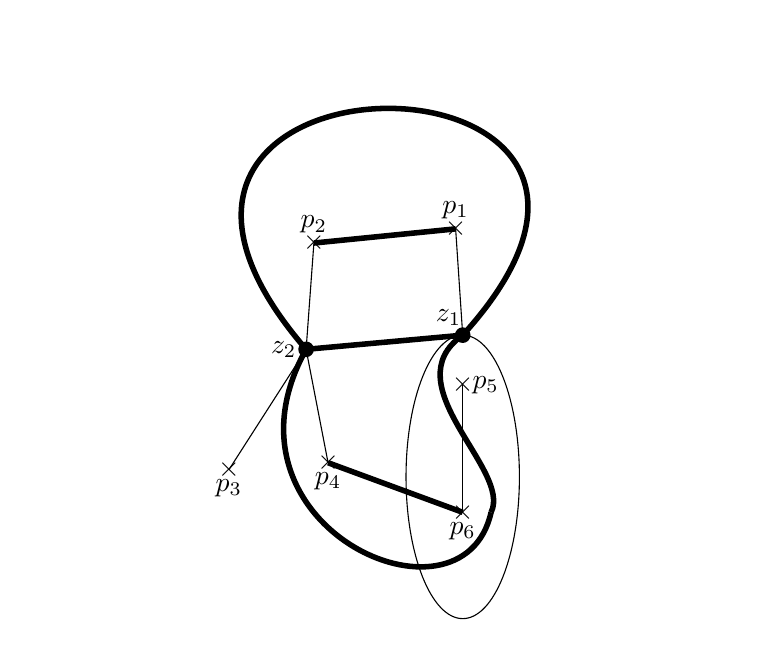
\begin{tikzpicture}[scale=0.9]
        \draw (0,0)--(-0.11,-1.5)--(-1.2,-3.2);
        \draw (-0.11,-1.5)--(0.2,-3.1);
        \draw (2.1,-3.3) ellipse (0.8cm and 2.0cm);
        \draw (2.1,-1.3)--(2.0,0.2);
        \draw (2.1,-2)--(2.1,-3.8);
         \node[ circle, fill=black,inner sep = 2pt] (A) at (-0.11,-1.5){};
        \node[ circle, fill=black,inner sep = 2pt] (A) at (2.1,-1.3){};
         \node at(0,0){$\times$}; 
        \node  at(-1.2,-3.2){$\times$};
        \node  at(0.2,-3.1){$\times$}; 
       \node  at(2.0,0.2){$\times$}; 
        \node  at(2.1,-2){$\times$}; 
        \node  at(2.1,-3.8){$\times$}; 
        \node[left] at (-0.11,-1.5) {$z_2$};
        \node[above] at (1.9,-1.3) {$z_1$};
         \node[above] at(0,0){$p_2$};
         \node[above] at(2,0.2){$p_1$};
           \node[right] at(2.1,-2){$p_5$};
             \node[below] at(2.1,-3.8){$p_6$};
         \node[below] at(-1.2,-3.2){$p_3$};
         \node[below] at(0.2,-3.1){$p_4$};
         \draw[line width=2pt] (0,0) -- (2,0.2);
          \draw[line width=2pt] (-0.11,-1.5) -- (2.1,-1.3);
          \draw[line width=2pt] (-0.11,-1.5) .. controls (-4,3) and (6,3).. (2.1,-1.3);
            \draw[line width=2pt] (0.2,-3.1) -- (2.1,-3.8);
    \draw[line width=2pt]  (-0.11,-1.5) .. controls (-1.5, -4) and (2.1, -5.6) .. (2.5,-3.8);
     \draw[line width=2pt] (2.1,-1.3) .. controls (1.1,-2) and (2.8,-3.2) .. (2.5,-3.8) ;
    \end{tikzpicture}

\caption{Thick lines denote vertical leaves. There are two vertical cylinders, with closed leaves surrounding $\widehat{p_1p_2}$ and $\widehat{p_4p_6}$, respectively. }
       \label{fig:I-7-3} 
\end{figure}





Similar to the subcase before, we 
have a vertical cylinder $\Theta_1$ with close leaves surrounding $\widehat{p_1p_2}$. Since $|\gamma_1|= |\gamma_2|$, both $z_1$ and $z_2$ lie on the boundary of $\Theta_1$.
On the other hand, there is a vertical cylinder $\Theta_2$ with close leaves surrounding $\widehat{p_4p_6}$. Since $|\gamma_4|< |\alpha|$, the boundary of $\Theta_2$ must meets $z_2$.
So  $\Theta_2$ must be bounded by a union of two vertical saddle connections, each of which connects $z_1$ and $z_2$. 
This is illustrated in Figure \ref{fig:I-7-1}. 

 Now the complement of $\overline{\Theta_1}\cup \overline{\Theta_2}$ is a Jordan domain $\Omega$, which contains the two poles $p_3$ and $p_5$. 
Thus the vertical foliation of $\phi$ is Jenkins-Strebel.  By applying the
$\rot$-action on $\phi$, we can reduce $\phi$ to the
Case (I-2).

The remaining subcase is that $|\gamma_1|> |\gamma_2|$. 
First we assume that $|\gamma_2|>|\alpha|$. 
By appropriately shearing $\phi$  along the horizontal cylinders we can assume that $p_2$
and $p_6$ is connected by a vertical saddle connection, and $z_1$ is connected by a vertical saddle connection to $p_5$. Denote the above vertical saddle connections by $\widehat{p_2p_6}$
and $\widehat{z_1p_5}$, respectively.
This is illustrated in Figure \ref{fig:I-7-2}. 



\begin{figure}[h!]
\centering
\includegraphics[scale=0.4]{fig7c}
\caption{Thick lines denote vertical leaves. There is a vertical cylinder with close leaves surrounding $\widehat{p_2p_6}$ and bounded by $\delta$. }
       \label{fig:I-7-2} 
\end{figure}

Consider the vertical cylinder $\Theta_1$ with leaves surrounding 
$\widehat{p_2p_6}$.
Since $|\gamma_2|>|\alpha|$, $z_1$ is contained in the boundary of $\Theta_1$. 
Moreover, $\overline{\Theta_1}$ is bounded by a vertical closed saddle connection
passing through $z_1$, denoted by  $\delta$. 
Since $z_1$ is a simple zero, the remaining angle at $z_1$ outside $\Theta_1$ is $\pi$.
As a result, there must be another vertical cylinder $\Theta_2$ adjoint to $\Theta_1$. The cylinder 
$\Theta_2$ is bounded by $\delta$ and another vertical  closed saddle connection passing through 
$z_2$. The complement of $\overline{\Theta_1} \cup \overline{\Theta_2}$ is a Jordan domain containing at most three poles. Replace $\phi$ by $\rot\cdot \phi$. Either $\Omega$ corresponds to the third horizontal cylinder or we can apply Theorem \ref{thm:SW} to produce a new Jenkins-Strebel differential $\psi$ in $\overline{H\cdot \phi}$ with three horizontal cylinders. 



Now we assume that $|\alpha|\geq |\gamma_2|$. By our assumption, 
$|\alpha|\geq |\gamma_2|\geq |\gamma_3|\geq |\gamma_4.$ The inequality together with Equation \ref{equ:length} implies $|\gamma_3|+|\gamma_4|\geq |\gamma_1|$ or, equivalently, 
$|\gamma_1|-|\gamma_3| \leq |\gamma_4|$. 
By appropriately shearing $\phi$  along the horizontal cylinders,  we can assume that $p_3$
and $p_1$ is connected by a vertical saddle connection, and $z_2$ is connected by a vertical saddle connection to $p_6$. Denote the above vertical saddle connections by $\widehat{p_1p_2}$
and $\widehat{z_2p_6}$, respectively. Let $\Theta_1$ be the vertical cylinder with closed leaves surrounding $\widehat{p_1p_2}$, which is bounded by a vertical closed saddle connection passing through $z_2$. 

Now we examine the neighborhood of $\overline{\Theta_1}\cup \widehat{z_2p_6}$.
Since $|\gamma_1|-|\gamma_3| \leq |\gamma_4|\leq |\gamma_2|\leq |\alpha|$, there must be a vertical cylinder 
$\Theta_2$ adjoint to $\Theta_1$, which is illustrated in Figure \ref{fig:I-7-3}.
The width of $\Theta_2$ is $|\gamma_1|-|\gamma_3|$. It crosses $\gamma_2$, $\gamma_4$
and $\alpha$. Note that the complement of $\overline{\Theta_1}\cup \widehat{\Theta_2}$ is non-empty.
For otherwise, $|\gamma_2|=|\gamma_3|=|\gamma_4|=|\alpha|$, which implies $|\gamma_1|=|\gamma_2|$,
which is contradicted to our assumption that $|\gamma_1|> |\gamma_2|$. 
 Replace $\phi$ by $\rot\cdot \phi$.
 Now either the complement of $\overline{\Theta_1}\cup \overline{\Theta_2}$ corresponds to the third horizontal cylinder or we can apply Theorem \ref{thm:SW} to produce a new Jenkins-Strebel differential $\psi$ in $\overline{H\cdot \phi}$ with three horizontal cylinders. 

\begin{figure}[h!]
\centering
\includegraphics[scale=0.3]{fig7b}
\caption{Thick lines denote vertical leaves. The grey cylinder is $\Theta_2$. }
       \label{fig:I-7-3} 
\end{figure}






%Case 8: One of the horizontal rays emanating from one zero terminates at another zero. There are two horizontal segments connecting the first zero and two poles and there is a horizontal segment emanating from the second zero terminates at itself. There are two remaining  pairs of poles; each pair is joined by a horizontal segment.(See Figure 11 : Case 5)
%\begin{figure}
   % \centering
   % \includegraphics[width=0.7\linewidth]{11.jpg}
    %\caption{Case 5}
   % \label{fig:enter-label}
%\end{figure}

%The $\epsilon-$ neighborhood of $\Gamma$ has four boundary components. $\phi$ is Jenkins-Strebel with two cylinders.

%By shearing $\phi$ appropriately, we may assume that there is a vertical geodesic connecting a pole to another pole. Then $\phi$ has two vertical cylinders which are not dense in $S_{0,6}$. So by Theorem 2.3 (b), the horocycle orbit closure of the rotated differential 
%$$\begin{pmatrix}
    %0 & -1\\
   % 1 & 0
%\end{pmatrix}\cdot\phi$$
%contains a Jenkins-Strebel differential with three cylinders.\\

%Case 6: One of the horizontal rays emanating from one zero terminates at another zero. There are four horizontal segments connecting the  zeros and four poles. and there is a horizontal segment connecting two remaining  poles;(See Figure 12: Case 6)


%\begin{figure}
  %  \centering
   % \includegraphics[width=0.6\linewidth]{12.jpg}
   % \caption{Case 6}
    %\label{fig:enter-label}
%\end{figure}

%The $\epsilon-$ neighborhood of $\Gamma$ has two boundary components. $\phi$ is Jenkins-Strebel with one cylinder.

%By shearing $\phi$ appropriately, we may assume that there is a vertical geodesic connecting a pole in one component to one pole in another component.Then $\phi$ has two vertical cylinders which are not dense in $S_{0,6}$. Similar to Theorem 2.3(b), the horocycle orbit closure of the rotated differential 
%$$\begin{pmatrix}
    %0 & -1\\
    %1 & 0
%\end{pmatrix}\cdot\phi$$
%contains a Jenkins-Strebel differential with three cylinders.
\subsubsection*{\textbf{(I-6-b):}} See Figure \ref{fig:I-7-b} for an illustration. 
In this case we have the equation 
$|\alpha|=\sum\limits_{i=1}^{4}|\gamma_i|$.
By  appropriately shearing the horizontal cylinders, we may assume that $p_1$  is connected to $p_5$ by a vertical saddle connection, $z_1$
is connected to $p_4$ by a vertical saddle connection.

Now, there exists a vertical cylinder $\Theta_1$ with closed leaves surrounding the vertical saddle connection $\widehat{p_1p_5}$. The domain $\overline{\Theta_1}$ is bounded by a vertical closed saddle connection passing through $z_1$. Denote such a  vertical closed saddle connection by $\delta$. 
Since $|\alpha|-|\gamma_1|\geq |\gamma_4|$ and $|\gamma_2|\geq |\gamma_3|\geq |\gamma_4|$,
there exists a second vertical cylinder $\Theta_2$ adjoint to $\Theta_1$ with width $|\gamma_4|$, which crosses $\gamma_2, \gamma_3$ and $\alpha$. 

Replace $\phi$ by $\rot \cdot \phi$. Now either the  complement of $\overline{\Theta_1} \cup \overline{\Theta_2}$ corresponds to the third horizontal cylinder or we can apply Theorem \ref{thm:SW} to produce a new Jenkins-Strebel differential $\psi$ in $\overline{H\cdot \phi}$ with three horizontal cylinders. 



\begin{figure}[h]
    \centering
    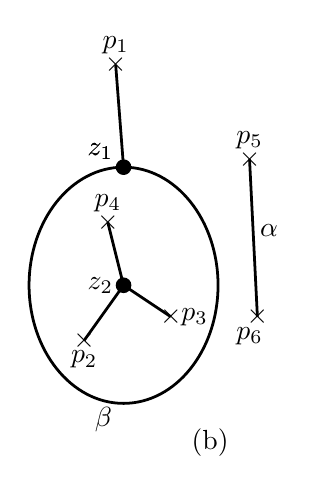
\begin{tikzpicture}[line width=1pt,scale=1]
        
        \draw (5.2,-2.3) ellipse (1.2cm and 1.5cm);
        %\draw (2.1,-1.3)--(2.0,0);
        %\draw (2.1,-2)--(2.1,-2.8);
        \draw (5.2,-0.8)--(5.1,0.5);
        \draw (5.2,-2.3)--(5.0,-1.5);
        \draw (5.2,-2.3)--(4.7,-3);
        \draw (5.2,-2.3)--(5.8,-2.7);
        \draw (6.8,-0.7)--(6.9,-2.7);
         \node[ circle, fill=black,inner sep = 2pt] (A) at (5.2,-0.8){};
        \node[ circle, fill=black,inner sep = 2pt] (A) at (5.2,-2.3){};
         \node  at(5.1,0.5){$\times$}; 
        \node  at(5.0,-1.5){$\times$};
        \node  at(4.7,-3){$\times$}; 
       \node  at(5.8,-2.7){$\times$}; 
        \node  at(6.8,-0.7){$\times$}; 
        \node  at(6.9,-2.7){$\times$}; 
        \node at (6.3,-4.3) {(b)};
           \node[left] at (5.2,-0.6) {$z_1$};
           \node[left] at (5.2,-2.3) {$z_2$};
             \node[left] at (5.2,-0.6) {$z_1$};
        \node[above] at (5.1,0.5) {$p_1$};
        \node[right] at (6.8,-1.6) {$\alpha$};
         \node[above] at (6.8,-0.7) {$p_5$};
           \node[below] at (6.8,-2.7) {$p_6$};
        \node[right] at (4.7,-4) {$\beta$};
           \node[above] at (5.0,-1.5) {$p_4$};
           \node[right] at (5.8,-2.7) {$p_3$};
            \node[below] at (4.7,-3) {$p_2$};
    \end{tikzpicture}

\caption{Case (I-6-b). }

       \label{fig:I-7-b} 
\end{figure}






\medskip
\noindent
{\bf Jenkins-Strebel differentials with a single cylinder.}

\subsection*{Case \textbf{(I-7):}}  The two zeros of $\phi$ are connected by a unique horizontal saddle connection, and each zero is connected to two poles by horizontal saddle connection, see Figure \ref{fig:I-4}. Denote the saddle connection between the two zeros by $\alpha$. There is a horizontal connection ending at two poles, denoted by $\beta$.

\begin{figure}[h]
    \centering
    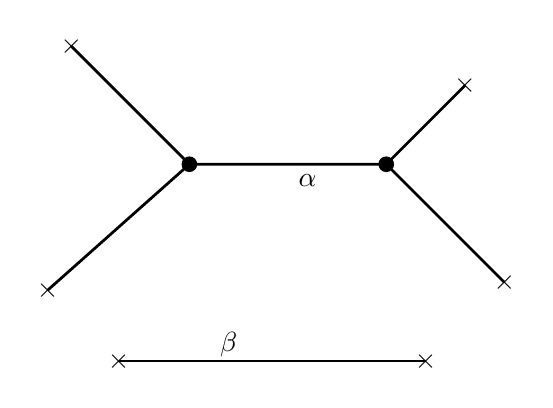
\begin{tikzpicture}[line width=1pt]
        \draw (0,0)--(1.5,-1.5)--(4,-1.5)--(5,-0.5);
        \draw (-0.3,-3.1)--(1.5,-1.5);
        \draw (4,-1.5)--(5.5,-3);
        \node[ circle, fill=black,inner sep = 2pt] (A) at (1.5,-1.5){};
        \node[ circle, fill=black,inner sep = 2pt] (A) at (4,-1.5){};
        \draw (0.6,-4.0)--(4.5,-4.0);
        \node  at(0,0){$\times$}; 
        \node  at(5,-0.5){$\times$};
        \node[below] at (3,-1.5) {$\alpha$};
         \node[below] at (2,-3.5) {$\beta$};
          %\node[right] at (0,-2) {$\gamma_1$};
          % \node at (5,-2) {$\gamma_2$};
\node  at(-0.3,-3.1){$\times$}; 
\node  at(0.6,-4.0){$\times$}; 
\node  at(4.5,-4.0){$\times$}; 
        \node at(5.5,-3){$\times$};
    \end{tikzpicture}
\caption{Case (I-7).}
       \label{fig:I-4}
\end{figure}



In this case,  $\phi$ is a Jenkins-Strebel differential with a single horizontal cylinder. 
Note that $|\alpha| < |\beta|$. By appropriately
shearing the horizontal cylinder, we may assume that each zero is connected  to itself by  a vertical saddle connection. The two vertical saddle connections together bound a vertical cylinder $\Theta$,
and the complement of $\overline{\Theta}$ consists of two Jordan domains.
In each such Jordan domain, there are three poles. 

Replace $\phi$ by $\rot \cdot \phi$. Now either each  complement component of $\overline{\Theta}$ corresponds to a horizontal cylinder 
or we can apply Theorem \ref{thm:SW} to produce a new Jenkins-Strebel differential $\psi$ in $\overline{H\cdot \phi}$ with three horizontal cylinders. 


\subsection*{Case \textbf{(I-8):}} This is the final case, illustrated in Figure \ref{fig:I-8}.
 Each zero is connected to three poles by horizontal saddle connections. 
 By  appropriately shearing this horizontal cylinder, we can assume that 
 $p_1$ and $p_4$ are connected by  a vertical saddle connection.
 
 Denote by $\gamma_1, \gamma_2$ and $\gamma_3$ the horizontal saddle connections joining
 $z_1$ to $p_1, p_2$ and $p_3$, respectively.  Denote by $\gamma_4, \gamma_5$ and $\gamma_6$ the horizontal saddle connections joining
 $z_2$ to $p_4, p_5$ and $p_6$, respectively. 
 Then we have the equation 
 $$|\gamma_1|+|\gamma_2|+|\gamma_3|= |\gamma_4|+|\gamma_5|+|\gamma_6|.$$
 
 If all $\gamma_i$ have equal length, then by using the $\rot$-action the resulting quadratic differential
 is exactly the same as the one in Case (I-3). As a result, by abuse of notation,
  we can assume that $|\gamma_1|> |\gamma_4|$. Since $p_1$ and $p_4$ are connected by  a vertical saddle connection, there exists a vertical cylinder $\Theta$ with closed leaves 
 surrounding the  vertical saddle connection $\widehat{p_1p_4}$. 
 
 Replace $\phi$ by $\rot\cdot \phi$. 
 Now either the horizontal foliation of $\phi$ is Jenkins-Strebel or we can apply Theorem \ref{thm:SW} to produce a new Jenkins-Strebel differential $\psi$ in $\overline{H\cdot \phi}$ with two or three horizontal cylinders. Thus,  we can reduce $\phi$ to  the previous cases.
 



\begin{figure}[h]
    \centering
    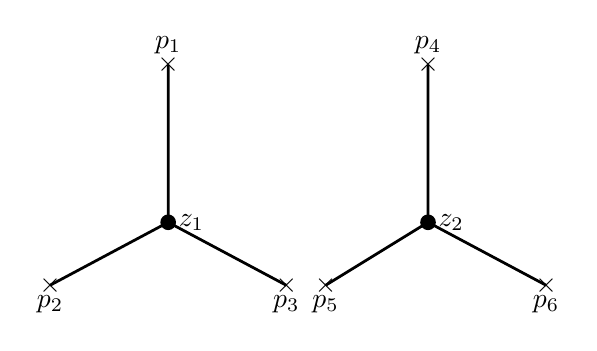
\begin{tikzpicture}[line width=1pt]
        \draw (0,0)--(0,-2)--(-1.5,-2.8);
        \draw (0,-2)--(1.5,-2.8);
        \draw (3.3,0)--(3.3,-2)--(2,-2.8);
        \draw (3.3,-2)--(4.8,-2.8);
        \node[ circle, fill=black,inner sep = 2pt] (A) at (0,-2){};
        \node[ circle, fill=black,inner sep = 2pt] (A) at (3.3,-2){};
         \node  at(0,0){$\times$}; 
        \node  at(-1.5,-2.8){$\times$};
        \node  at(1.5,-2.8){$\times$}; 
       \node  at(3.3,0){$\times$}; 
        \node  at(2,-2.8){$\times$}; 
        \node  at(4.8,-2.8){$\times$}; 
          \node[above]  at(0,0){$p_1$}; 
        \node[below]  at(-1.5,-2.8){$p_2$};
        \node[below]  at(1.5,-2.8){$p_3$}; 
       \node[above]  at(3.3,0){$p_4$}; 
        \node[below]  at(2,-2.8){$p_5$}; 
        \node[below]  at(4.8,-2.8){$p_6$}; 
        \node[right]  at(0,-2){$z_1$}; 
          \node[right]  at(3.3,-2){$z_2$};
        %\node at (1.8,-3.3) {(b)};
    \end{tikzpicture}
    \caption{ Case (I-8).}
    \label{fig:I-8}
\end{figure}








%\begin{figure}
    %\centering
    %\includegraphics[width=0.5\linewidth]{8.1.jpg}
    %\caption{Case 8}
    %\label{fig:enter-label}
%\end{figure}


We conclude from the above discussion that

\begin{Proposition}\label{prop:staircase}
Let $\phi\in \Q(1^2, -1^6)$. There exists a Jenkins-Strebel differential $\psi\in \Q(1^2, -1^6)$ 
such that 
\begin{itemize}
  \item $\psi$ is a staircase.
  \item If $\tau^\phi$ admits a holomorphic retraction, so does $\tau^\psi$. 
\end{itemize}
\end{Proposition}





\subsection{Case (II): $\Q(2, -1^6)$.}\label{Case-II}

There is a canonical double cover $\eta: S_{2,0} \to S_{0,6}$
branched over the marked points. By pulling back
Riemann surface structures, $\eta$ induces a holomorphic isometry  of Teichm\"uller spaces (with respect to the Teichm\"uller metric)
$$\eta^* : \Tei_{0,6} \cong \Tei_{2,0}.$$
Moreover, any quadratic differential on $X\in \Tei_{0,6}$ is pulled back  to a 
quadratic differential $\psi$ on $Y= \eta^*(X)$. 

\begin{figure}[h]
    \centering
    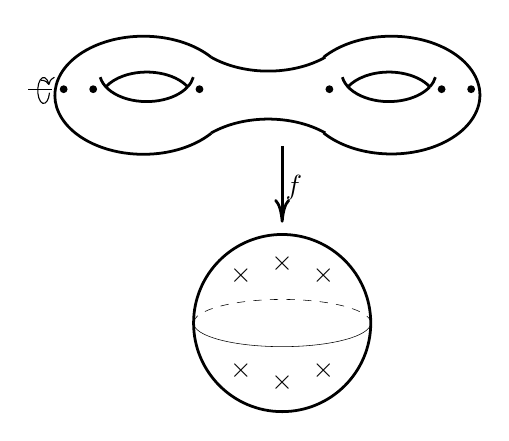
\begin{tikzpicture}[line width=1pt,scale=0.75]

        \draw [line width=1pt] (-1.2,4.5) arc (40:320:1.5cm and 1.0cm);       
        %\draw [line width=1pt] (-0.5,4.5) arc (180:180:1.5cm and 1.0cm);         
       \draw [line width=1pt] (-1.2,4.5) arc (230:310:1.5cm and 1.0cm);
        \draw [line width=1pt] (-1.2,3.22) arc (130:50:1.5cm and 1.0cm);     
        \draw [line width=1pt] (+0.7,4.5) arc (140:0:1.5cm and 1.0cm);         
       \draw [line width=1pt] (+0.7,3.22) arc (220:360:1.5cm and 1.0cm);  
      \draw [line width=1pt] (-1.6,4) arc (30:150:0.8cm and 0.5cm);
    \draw [line width=1pt] (-1.6,4) arc (330:190:0.8cm and 0.5cm);
    \draw [line width=1pt] (-1.6,4) arc (330:350:0.8cm and 0.5cm);
     \draw [line width=1pt] (2.5,4) arc (30:150:0.8cm and 0.5cm);
    \draw [line width=1pt] (2.5,4) arc (330:190:0.8cm and 0.5cm);
    \draw [line width=1pt] (2.5,4) arc (330:350:0.8cm and 0.5cm);
    \draw [line width=1pt][-{To[length=3mm,width=2mm]}] 
    (0,3)--(0,1.7);
    \node at (0.2,2.3) {$f$};
    \node [ circle, fill=black,inner sep = 1pt] (A) at (-3.7,3.96) {};
     \node [ circle, fill=black,inner sep = 1pt] (A) at (-3.2,3.96) {};   
    \node [ circle, fill=black,inner sep = 1pt] (A) at (-1.4,3.96) {};
     \node [ circle, fill=black,inner sep = 1pt] (A) at (0.8,3.96) {};
    \node [ circle, fill=black,inner sep = 1pt] (A) at (2.7,3.96) {};
    \node [ circle, fill=black,inner sep = 1pt] (A) at (3.2,3.96) {};
    \draw [line width=0.4pt](-4.3,3.96)--(-3.9,3.96); 
    \draw [line width=0.4pt][->] (-3.94,3.9) arc (350:25:0.1cm and 0.22cm);      
        \draw [line width=1pt](0,0) circle (1.5);
        \draw [line width=0.2pt,dashed] (1.5,0) arc (0:180:1.5cm and 0.4cm);
        \draw [line width=0.2pt] (-1.5,0) arc (180:360:1.5cm and 0.4cm);
        \node at (0.7,0.8){$\times$};
        \node at (0,1){$\times$};
        \node at (-0.7,0.8){$\times$};
        \node at (0.7,-0.8){$\times$};
        \node at (0,-1){$\times$};
        \node at (-0.7,-0.8){$\times$};
    \end{tikzpicture}
        \caption{The canonical double cover $\eta: S_{2,0}\to S_{0,6}$.}
    \label{fig:enter-label}
\end{figure}


If $(X,\phi)\in \Q(2, -1^6)$, then  $(Y,\psi)$ be a holomorphic quadratic differential in $Q\Tei_{2,0}$, which has two zeros of even order. 
According to Kra's theorem, there exists a holomorphic retraction 
$$F: \Tei_{2,0} \to \mathbb{H}, \  F \circ \tau^\psi= \operatorname{id}_{\mathbb{H}}.$$
As a consequence, $\tau^\phi$ admits a holomorphic retraction. 


\subsection{Case (III): $\Q(1, -1^5)$.}\label{Case-III}
There are two subcases.

\subsection*{Case (III-1):} The zero of $\phi$ does not lie at a marked point. 
In this case, $\phi$ is a Jenkins-Strebel differential with a simple zero. There are two  possibilities, see Figure \ref{fig:III-1} for an illustration. The right one can be transform into the left one.

\begin{figure}[h]
\centering

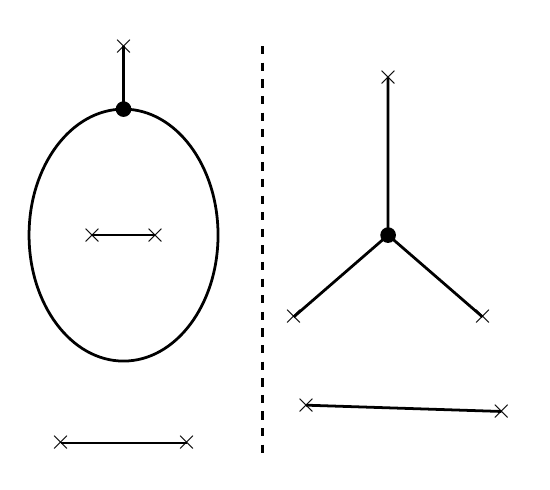
\begin{tikzpicture}[line width=1pt,scale=0.8]
%[every node/.style = {draw, circle, inner sep = 2pt}]
  % 圆形：圆心在 (0,0)，半径为 1.5cm
 % \node (A) at (0,0);
 
  \draw (-4.2,0) ellipse (1.5cm and 2cm);
  \node[ circle, fill=black,inner sep = 2pt] (A) at (-4.2, 2.0){};
  \draw (-4.2,2.0) to (-4.2,3.0);
      \node  at (-4.2, 3){$\times$};
   \draw (-4.7,0) to (-3.7,0);
    \node  at (-4.7, 0){$\times$};
     \node at (-3.7, 0){$\times$};
     \draw (-5.2,-3.3) to (-3.2, -3.3);
      \node at (-5.2, -3.3){$\times$};
     \node  at (-3.2, -3.3){$\times$};
     \draw[dashed] (-2,3)--(-2,-3.5);
     \draw (0,2.5)--(0,0)--(-1.5,-1.3);
        \draw (0,0)--(1.5,-1.3);
     \draw (-1.3,-2.7)--(1.8,-2.8);
\node at (0,2.5){$\times$};
     \node  at (1.5,-1.3){$\times$};

     \node at (-1.5,-1.3){$\times$};
     \node  at (-1.3,-2.7){$\times$};
     \node at (1.8,-2.8){$\times$};
\node[ circle, fill=black,inner sep = 2pt] (A) at (0,0){};
     
\end{tikzpicture}
%\lable{fig:a}
\caption{Case (III-1).}
\label{fig:III-1}
\end{figure}


Let us assume that $\phi$ is the one on the left of Figure \ref{fig:III-1}.
In this situation, we shall consider the regular marked point on $S_{0,6}$ as a singularity of order $0$. That is,  $\phi$ is a quadratic differential in the stratum 
$\Q(1, -1^5, 0)$. 

There is a horizontal closed saddle connection $\gamma$ joining the zero to itself,
which separates the surface into two horizontal cylinders $\Pi_1$ and $\Pi_2$.  
We can use the $\mathbb{H}^2$-action to shear $\phi$ appropriately along the horizontal cylinders so that $\phi$ is a $L$-shaped pillowcase  with an extra marked point. See Figure \ref{fig:III-2} for an illustration, where we denote the zero by $z$, the poles by $p_1, \cdots, p_5$ and the extra marked point by $p$. 
Without loss of generality, we may assume that $p$ lies in the closure of $\Pi_2$.

\begin{figure}[h]
    \centering
   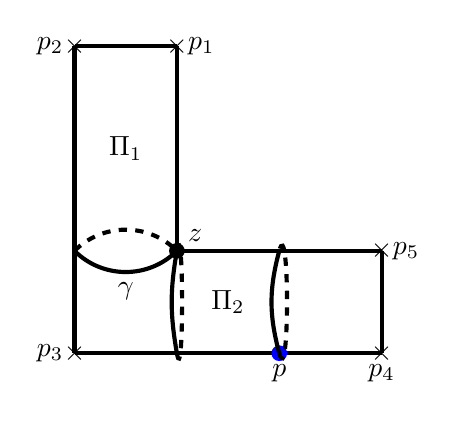
\begin{tikzpicture}[line width=1.5pt,scale=1.3]
        \node[circle, fill=black,inner sep = 2pt] (A) at (0,0){};
       \node  at(0,2){$\times$};
       \node  at(-1,2){$\times$};
      \node at(2,0){$\times$};
      \node at(2,-1){$\times$};
      \node at(-1,-1){$\times$};
      \draw (0,0) -- (2,0);
      \draw (0,0) -- (0,2);
      \draw (0,2) -- (-1,2);
      \draw (-1,2) -- (-1,-1);
      \draw (-1,-1) -- (2,-1);
      \draw (2,-1) -- (2,0);
       \node[below] at (-0.5,-0.2){$\gamma$};
       \draw (-1,0) to[out=315,in=225] (0,0);
         \draw[dashed] (-1,0) to[out=45,in=135] (0,0);
           \draw (0,-1) to[out=100,in=260] (0,0);
         \draw[dashed] (0,-1) to[out=280,in=80] (0,0);
          \node[circle, fill=blue,inner sep = 2pt] (A) at (1,-1){};
          \node[below] at (1,-1){$p$};
          \draw (1,-1) to[out=105,in=255] (1,0);
          \draw[dashed] (1,-1) to[out=285,in=75] (1,0);
      \node at (0.5,-0.5){$\Pi_2$};
      \node at (-0.5,1){$\Pi_1$};
      \node[right] at (0,0.15) {$z$};
       \node[right]  at (0,2) {$p_1$};
       \node[left]  at(-1,2){$p_2$};
      \node[right] at(2,0){$p_5$};
      \node[below] at(2,-1){$p_4$};
      \node[left] at(-1,-1){$p_3$}; 
   \end{tikzpicture}
   \caption{The Jenkins-Strebel differential in Case (III-1), which can be deformed into a L-shaped pillowcase with an extra marked point (the blue bullet) lying at the bottom.}
   \label{fig:III-2}
\end{figure}


If $p$ lies in the interior of $\Pi_2$, then we can take the  horizontal closed trajectory of $\phi$
passing through $p$, which together with $\gamma$ separate the surface into three horizontal cylinders. By using the 
action of $\mathbb{H}^3$ on the horizontal cylinders, we can move the marked point $p$ such that it lies at the left side of the $L$-shaped polygon. Rotating $\phi$ by $\rot$, we can transform $\phi$ into a $L$-shaped pillowcase such that the marked point $p$ lies at the bottom of the polygon.

If $p$ lies at the saddle connection between $z$ and $p_5$ (but not at the saddle connection between $p_3$ and $p_4$), then we add the  vertical closed trajectory of $\phi$
passing through $p$ and consider $\phi$ as a Jenkins-Strebel differential with three vertical cylinders. Rotate $\phi$ by $\rot$ and apply the $\mathbb{H}^3$-action to $\rot \cdot \phi$
we can move $p$ to the bottom of $\phi$. 


Finally, assume that the marked point $p$ lies at $\gamma$ (but not at the saddle connection between $p_2$ and $p_3$). We take the vertical closed leaf passing through $p$ and consider
$\phi$ as a Jenkins-Strebel differential with three vertical cylinders. 
Up to the $\rot$-action, we can again transform $\phi$ into a $L$-shaped pillowcase such that the marked point $p$ lies at the bottom of the polygon.

As a result, we can always assume that $\phi$ is the double of a $L$-shaped polygon
with an extra marked point lying at the bottom. We can deal with this case 
using Markovic's computation for the $L$-shaped polygon \cite{Markovic2018}.
This is the same as for the proof of \cite[Theorem 1.1]{Markovic2018}, which shows that 
 $\tau^\phi$ does not admit a holomorphic retraction. We omit the details.








\subsection*{Case (III-2):}  The zero of $\phi$ is a marked point. 
In this case, the pullback of  $\phi$ under $\eta^*$ gives a quadratic differential
$\psi$ with a single zero of order $4$ on $S_{2,0}$. By Kra's theorem,  $\tau^{\phi}$ admits a holomorphic retraction. 


\subsection{Case (IV): $\Q(-1^4)$.}\label{Case-IV}
In this case, the pullback of  $\phi$ under $\eta^*$ produces a quadratic differential
$\psi$ with two zeros of order $2$ on $S_{2,0}$. By Kra's theorem,  $\tau^{\phi}$ admits a holomorphic retraction. 


\subsection{Conclusion}

From the above discussion, to prove Theorem \ref{thm:main2}, it suffices to show that 
 the equation \eqref{equ:criterion} does not hold for  staircase Jenkins-Strebel differentials.  This will be addressed in Section \ref{sec:computation}.
 

To prove Theorem \ref{thm:main}, we can identify any quadratic differential 
$\psi$ on a genus two surface as the pullback of some $\phi\in Q\Tei_{0,6}$. 
Note that if $\psi$ has a zero of odd order, then either $\phi\in \mathcal{Q}(1^2,-1^6)$ or  $\phi\in \mathcal{Q}(1,-1^5)$. In the latter case,
the zero of $\phi$ could not be located at a marked point. Thus Theorem \ref{thm:main}
follows directly from Theorem \ref{thm:main2}.





\section{Staircase surfaces} \label{sec:computation}
\noindent

We have already shown in Section \ref{sec:classify}  that
the proof of Theorem \ref{thm:main2} can be reduced to staircase surfaces. 
In this section, we  show that for any  given staircase on $S_{0,6}$, the associated Teichm\"uller disk does not
admit a holomorphic retraction. 
Our result generalizes Markovic's previous work on $L$-shaped pillowcases \cite{Markovic2018}. 


\begin{Remark}
  Markovic's computation shows that extremal length is not $C^2$ along certain smooth paths in  the space of measured foliations, see also Azemar \cite[Theorem 1.9]{Azemar}.
\end{Remark}


\subsection{Holomorphic retraction}\label{sec:area}

Let us begin with some notation. Assume that $a, b, c>0$ and $p,q>0, p+q<1$.
 Let $L(a,b,c,p,q)$ be a staircase-shaped polygon as shown in Figure \ref{fig:L1}.
 There are six vertices, denoted by
 $P_k, k=1, \cdots,6$, at which the interior angles are $\frac{\pi}{2}$. And there are another two vertices, denoted by $Q_1$ and $Q_2$, at which the interior angles are $\frac{3\pi}{2}$.


 Let $S(a,b,c,p,q)$ be the double of  $L(a,b,c,p,q)$,
  which is regarded as a Riemann sphere with  marked points $P_1, \cdots, P_6$.
Let $\phi(a,b,c,p,q)$ denote the quadratic differential on $S(a,b,c,p,q)$ obtained by 
gluing the two copies of $dz^2$ on $L(a,b,c,p,q)$. 
It is evident that $\phi(a,b,c,p,q)$ is a Jenkins-Strebel differential,
 with two simple zeros corresponding to $Q_1$ and  $Q_2$. The surface $S(a,b,c,p,q)$ is decomposed 
 by the horizontal critical graph of $\phi$ into three annuli $\Pi_1,\Pi_2$ and 
$\Pi_3$, each of which is swept out by horizontal closed  trajectories of $\phi(a,b,c,p,q)$.



 
\begin{figure}[h]
    \centering
    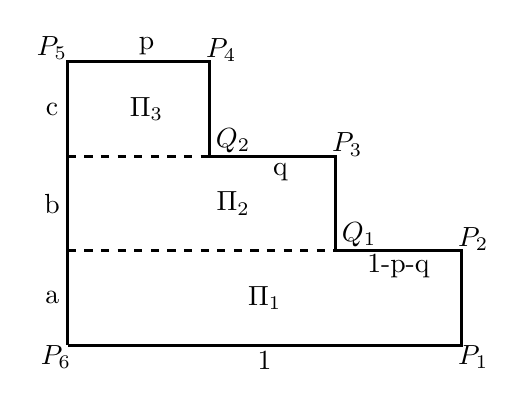
\begin{tikzpicture}[line width=1pt,scale=1]
        \draw (-5.7,0)--(-0.7,0)--(-0.7,1.2)--(-2.3,1.2)--(-2.3,2.4)--(-3.9,2.4)--(-3.9,3.6)--(-5.7,3.6)--(-5.7,0);
        \node at (-5.85,-0.15) {$P_6$};
        \node at (-0.55,-0.15){$P_1$};
        \node at (-0.55,1.35){$P_2$};
        \node at (-2.15,2.55){$P_3$};
        \node at (-3.75,3.75){$P_4$};
        \node at (-5.9,3.77){$P_5$};
        \node at (-2.0,1.4){$Q_1$};
        \node at (-3.6,2.6){$Q_2$};
        \draw[dashed] (-5.7,1.2)--(-2.3,1.2);
        \draw[dashed] (-5.7,2.4)--(-3.9,2.4);
        \node at (-3.2,-0.2){1};
        \node at (-1.5,1){1-p-q};
        \node at (-3,2.2){q};
        \node at (-4.7,3.8){p};
        \node at (-3.2,0.6){$\Pi_1$};
        \node at (-3.6,1.8){$\Pi_2$};
        \node at (-4.7,3){$\Pi_3$};
        \node at (-5.9,0.6){a};
        \node at (-5.9,1.8){b};
        \node at (-5.9,3){c};
    \end{tikzpicture}
    \caption{The polygon $L(a,b,c,p,q)$.}
    \label{fig:L1}
\end{figure}

%\begin{figure}
   % \centering
   % \includegraphics[width=0.7\linewidth]{1.jpg}
   % \caption{$L_1(a,b,c,p,q)$}
    %\label{fig:enter-label}
%\end{figure}

Fix $(a_0, b_0, c_0, p_0, q_0)$. We denote $S= S(a_0,b_0,c_0,p_0,q_0)$ and $\phi=\phi(a_0,b_0,c_0,p_0,q_0)$. 
The main result in this section is
 \begin{Theorem}\label{thm:typeA}
 The Teichm\"uller disk 
 $\tau^{\phi} : \mathbb{H} \to \Tei_{0,6}$ does not admit a holomorphic retraction.  
 \end{Theorem}
%We prove Theorem \ref{thm:typeA} by contradiction.


 To derive a contradiction, we assume that there exists a holomorphic retraction $$\Phi : \Tei_{0,6} \to \mathbb{H}$$ of the Teichm\"uller disk $\tau^{\phi}$. 
 Let $$\mathcal{E}:\mathbb{H}^3\rightarrow\Tei_{0,6}$$ be the Teichm\"uller polydisk associated with $\phi$. Define $$a_1=\frac{1}{{\|\phi\|}}\int_{\Pi_1}|\phi|=\frac{a_0}{a_0+b_0(p_0+q_0)+c_0p_0},$$
 $$a_2=\frac{1}{{\|\phi\|}}\int_{\Pi_2}|\phi|=\frac{b_0(p_0+q_0)}{a_0+b_0(p_0+q_0)+c_0p_0},$$ and
  $$ a_3=\frac{1}{{\|\phi\|}}\int_{\Pi_3}|\phi|=\frac{c_0p_0}{a_0+b_0(p_0+q_0)+cp_0}.$$
By Theorem \ref{thm:GM-JS}, we can assume that $\Phi$ satisfies  $$\left(\Phi\circ \mathcal{E}\right)(\lambda_1,\lambda_2,\lambda_3)=a_1\lambda_1+a_2\lambda_2+a_3\lambda_3$$
for all $(\lambda_1,\lambda_2,\lambda_3)\in \mathbb{H}^3$. 



Note that for any $a,b,c>0$, we have $$\mathcal{E}\left(\frac{a}{a_0}i,\frac{b}{b_0}i,\frac{c}{c_0}i\right)=S(a,b,c,p_0,q_0).$$ 
Thus we have the following equality \begin{equation}\label{equ:linear}
 \Phi(S(a,b,c,p_0,q_0))=\frac{a+b(p_0+q_0)+cp_0}{a_0+b_0(p_0+q_0)+c_0p_0}i.
\end{equation}


\begin{Lemma}\label{Lemma 4.2} Assume that the Teichm\"uller disk 
 $\tau^{\phi} : \mathbb{H} \to \Tei_{0,6}$ admits a holomorphic retraction. Then
there exists a holomorphic function $F$ on $\Tei_{0,6}$ such that $$F\left(S(a,b,c,p_0,q_0)\right)= a+b(p_0+q_0)+cp_0 $$ for every $a>0$ and $b,c\geq 0$.
\end{Lemma}

\begin{proof}
We take 
 $$F=\left( a_0+b_0(p_0+q_0)+c_0p_0\right) \frac{\Phi}{i},$$ which is a holomorphic function on $\Tei_{0,6}$. 
 By \eqref{equ:linear}, we have 
 $$F(S(a,b,c,p_0,q_0))= a+b(p_0+q_0)+cp_0$$ for any $a,b,c> 0$.
By continuity, the above equality holds for every $a>0$ and $b,c\geq 0$.
\end{proof}

Note that the function $F(S(a,b,c,p_0,q_0))$, for fixed $(p_0,q_0)$, is the area 
of  $L(a,b,c,p_0,q_0)$. 


\subsection{Computation of area.}\label{SCM}
Let $f:\mathbb{H} \to L(a,b,c,p,q)$ be the Riemann mapping such that $f(\infty)=P_1, f(-1)=P_2, f(1)=P_6$. Assume that
$f(\xi_1)=P_3, f(\xi_2)=P_4, f(\xi_3)=P_5$, where $-1<\xi_1<\xi_2<\xi_3<1$. Assume that 
$f(\eta_1)=Q_1, f(\eta_2)=Q_2$,  where $-1<\eta_1\leq\xi_1<\eta_2\leq\xi_2$ (we allow $b, c$
to be $0$). 
By  the Schwarz-Christoffel formula, $f$ is given by $$f(z)=J\int_1^z\frac{\sqrt{w-\eta_1}\sqrt{w-\eta_2}}{\sqrt{w-\xi_1}\sqrt{w-\xi_2}\sqrt{w-\xi_3}\sqrt{w-1}\sqrt{w+1}}dw.$$
Since $|P_6P_1|=1$, we have  $$\frac{1}{J}=\int_1^{\infty}\frac{\sqrt{x-\eta_1}\sqrt{x-\eta_2}}{\sqrt{x-\xi_1}\sqrt{x-\xi_2}\sqrt{x-\xi_3}\sqrt{x-1}\sqrt{x+1}}dx.$$

Since $S(a,b,c,p,q)$ is the double of $L(a,b,c,p,q)$, we can extend $f$ to a conformal mapping $$f: \mathbb{C}\setminus
\{-1,\xi_1,\xi_2,\xi_3,1\}\rightarrow S(a,b,c,p,q).$$ 

\subsection*{Computing the Schwarz-Christoffel maps.}

Consider the case that  $-1<\eta_1=\xi_1<\eta_2=\xi_2<\xi_3<1$. Under the Schwarz-Christoffel map,  the corresponding polygon is $L(a,0,0,p,q)$, which is a rectangle with two additional marked points $P_3$ and $P_4$ on the top side. Let $s>0$ and  $t>0$ be sufficiently small.
We deform $L(a,0,0,p,q)$ into a new polygon $$\mathbf{L}(s,t)=L\left(a(s,t),b(s,t),c(s,t),p(s,t),q(s,t)\right)$$ in a way that
the Schwarz-Christoffel map  
sends $(\xi_1, \xi_2, \xi_3)$ into $(P_3, P_4, P_5)$ and $(\xi_1-s, \xi_2-t)$ into $(Q_1, Q_2)$.  
In other words, we have $\eta_1=\xi_1-s, \eta_2=\xi_2-t$. Let $$\mathbf{S}(s,t)=S\left(a(s,t),b(s,t),c(s,t),p(s,t),q(s,t)\right)$$ be the double of $\TL(s,t)$, with the natural Jenkins-Strebel differential
$$\phi(s,t)=\phi\left(a(s,t),b(s,t),c(s,t),p(s,t),q(s,t)\right)$$
induced by the flat metric on $\TL(s,t)$.  
Note that the Riemann surface structure induced by $\TS(s,t)$ is  equivalent to  $\mathbb{C}\setminus
\{-1,\xi_1,\xi_2,\xi_3,1\}$.
So we obtain a  two-parameter family of Jenkins-Strebel differentials 
that represent the same point in $\Tei_{0,6}$. 

To compute $a(s,t), b(s,t), c(s,t), p(s,t), q(s,t)$, we let
\begin{eqnarray*}
% \nonumber % Remove numbering (before each equation)A(s,t)=-i\int_{-\infty}^{-1}\frac{\sqrt{x-\xi_1+s}\sqrt{x-\xi_2+t}}{\sqrt{x-1}\sqrt{x+1}\sqrt{x-\xi_1}\sqrt{x-\xi_2}\sqrt{x-\xi_3}}dx,$$
A(s,t)&=&-i\int_{-\infty}^{-1}\frac{\sqrt{x-\xi_1+s}\sqrt{x-\xi_2+t}}{\sqrt{x-1}\sqrt{x+1}\sqrt{x-\xi_1}\sqrt{x-\xi_2}\sqrt{x-\xi_3}}dx,\\
B(s,t)&=&-i\int_{\xi_1-s}^{\xi_1}\frac{\sqrt{x-\xi_1+s}\sqrt{x-\xi_2+t}}{\sqrt{x-1}\sqrt{x+1}\sqrt{x-\xi_1}\sqrt{x-\xi_2}\sqrt{x-\xi_3}}dx,\\
C(s,t)&=&-i\int_{\xi_2-t}^{\xi_2}\frac{\sqrt{x-\xi_1+s}\sqrt{x-\xi_2+t}}{\sqrt{x-1}\sqrt{x+1}\sqrt{x-\xi_1}\sqrt{x-\xi_2}\sqrt{x-\xi_3}}dx,\\
P(s,t)&=&-\int_{\xi_2}^{\xi_3}\frac{\sqrt{x-\xi_1+s}\sqrt{x-\xi_2+t}}{\sqrt{x-1}\sqrt{x+1}\sqrt{x-\xi_1}\sqrt{x-\xi_2}\sqrt{x-\xi_3}}dx,\\
Q(s,t)&=&-\int_{\xi_1}^{\xi_2-t}\frac{\sqrt{x-\xi_1+s}\sqrt{x-\xi_2+t}}{\sqrt{x-1}\sqrt{x+1}\sqrt{x-\xi_1}\sqrt{x-\xi_2}\sqrt{x-\xi_3}}dx,\\
\frac{1}{J(s,t)}&=&\int_{1}^{+\infty}\frac{\sqrt{x-\xi_1+s}\sqrt{x-\xi_2+t}}{\sqrt{x-1}\sqrt{x+1}\sqrt{x-\xi_1}\sqrt{x-\xi_2}\sqrt{x-\xi_3}}dx.
\end{eqnarray*}
It follows by definition that
\begin{eqnarray*}
% \nonumber % Remove numbering (before each equation)
  a(s,t) = {J(s,t)}{A(s,t)}, && 
  b(s,t) = {J(s,t)}{B(s,t)}, \ \ \ \ 
  c(s,t) ={J(s,t)}{C(s,t)}, \\
 p(s,t) = {J(s,t)}{P(s,t)}, &&   q(s,t)  = {J(s,t)}{Q(s,t)}.\\
\end{eqnarray*}

Both $J(s,t)$ and $A(s,t)$ are real analytic with respect to $(s,t)$,
 since their integrals depend analytically on $(s,t)$.
 
 \subsection*{Convention} We adopt the following convention. If two functions $h(s,t)$ and $g(s,t)$ satisfy $\frac{h(s,t)}{g(s,t)} \to 0$ as $(s,t)\to (0,0)$,
 then we denote $h(s,t)=o\left(g(s,t)\right)$.
 If there is a constant $C$ such that $\left|\frac{h(s,t)}{g(s,t)}\right| < C$, then
we denote $h(s,t)=O\left(g(s,t)\right)$.
 
\begin{Proposition}\label{prop:B-C}
With the about notation, we have for $s,t>0$ sufficiently small
    $$B(s,t)=\frac{\pi s}{2\sqrt{1-\xi_1}\sqrt{1+\xi_1}\sqrt{\xi_3-\xi_1}} +O(s^2)+O(st),$$
    $$C(s,t)=\frac{\pi t}{2\sqrt{1-\xi_2}\sqrt{1+\xi_2}\sqrt{\xi_3-\xi_2}}  +O(st)+ O(t^2).$$
\end{Proposition}
\begin{proof}
For $s,t>0$ sufficiently small, we have  for  $x\in[\xi_1-s,\xi_1]$
\begin{eqnarray*}
% \nonumber % Remove numbering (before each equation)
 \frac{-i}{\sqrt{x-1}\sqrt{x+1}\sqrt{x-\xi_3}} &=& \frac{i}{\sqrt{1-\xi_1}\sqrt{1+\xi_1}\sqrt{\xi_3-\xi_1}}+ O(s), \\
 \frac{\sqrt{x-\xi_2+t}}{\sqrt{x-\xi_2}} &=& 1+ O(t).
\end{eqnarray*}
 So we can write
\begin{eqnarray*}
% \nonumber % Remove numbering (before each equation)
  B(s,t) &=& \left(\frac{i}{\sqrt{1-\xi_1}\sqrt{\xi_1+1}\sqrt{\xi_3-\xi_1}}+O(s) \right)\int_{\xi_1-s}^{\xi_1}\frac{\sqrt{x-\xi_1+s}\sqrt{x-\xi_2+t}}{\sqrt{x-\xi_1}\sqrt{x-\xi_2}}dx \\
  &=& \left(\frac{i}{\sqrt{1-\xi_1}\sqrt{\xi_1+1}\sqrt{\xi_3-\xi_1}}+O(s) \right)\left(1+O(t)\right)
  \int_{\xi_1-s}^{\xi_1}\frac{\sqrt{x-\xi_1+s}}{\sqrt{x-\xi_1}}dx.
\end{eqnarray*}
It remains to compute the integral 
$$\int_{\xi_1-s}^{\xi_1}\frac{\sqrt{x-\xi_1+s}}{\sqrt{x-\xi_1}}dx.$$ Note that 
$$\int_{\xi_1-s}^{\xi_1}\frac{\sqrt{x-\xi_1+s}}{\sqrt{x-\xi_1}}dx=-i\int_{\xi_1-s}^{\xi_1}\frac{\sqrt{x-\xi_1+s}}{\sqrt{\xi_1-x}}dx,$$
Substituting $\xi_1-x=y$ then yields 
\begin{eqnarray*}
 -i\int_{\xi_1-s}^{\xi_1}\frac{\sqrt{x-\xi_1+s}}{\sqrt{\xi_1-x}}dx&=&-i\int_0^s\frac{\sqrt{s-y}}{\sqrt{y}}dy\\&=&-i\left[ \sqrt{s-y}\sqrt{y}+s\arctan\left( \frac{\sqrt{y}}{\sqrt{s-y}}\right)\right]\bigg|_0^s
 \\&=& -i\frac{\pi s}{2} . 
\end{eqnarray*}
We conclude that 
\begin{eqnarray*}
% \nonumber % Remove numbering (before each equation)
  B(s,t) &=& \left(\frac{1}{\sqrt{1-\xi_1}\sqrt{\xi_1+1}\sqrt{\xi_3-\xi_1}}+O(s) \right)\left(1+O(t)\right) \frac{\pi s}{2} \\
  &=& \frac{\pi s}{2\sqrt{1-\xi_1}\sqrt{1+\xi_1}\sqrt{\xi_3-\xi_1}}+ O(s^2) + O(st).
\end{eqnarray*}
The proof for $C(s,t)$ is similar.
\end{proof}

Recall that 
\begin{eqnarray*}
% \nonumber % Remove numbering (before each equation)
  P(0,0) &=& - \int_{\xi_2}^{\xi_3}\frac{1}{\sqrt{x-1}\sqrt{x+1}\sqrt{x-\xi_3}} dx,  \\
  Q(0,0) &=& - \int_{\xi_1}^{\xi_2}\frac{1}{\sqrt{x-1}\sqrt{x+1}\sqrt{x-\xi_3}} dx.  \\
\end{eqnarray*}
\begin{Proposition}\label{prop:P}
With the about notation, we have 
    $$P(s,t)-P(0,0)=\frac{1}{2\sqrt{1-\xi_2}\sqrt{1+\xi_2}\sqrt{\xi_3-\xi_2}} \  t\ln \frac{1}{t}+
    o\left( t \ln \frac{1}{t} \right) +O(s).$$
\end{Proposition}

\begin{proof} By definition, 
\begin{align*}
P(s,t)-P(0,0)  = \int_{\xi_2}^{\xi_3}\frac{1}{\sqrt{x-1}\sqrt{x+1}\sqrt{x-\xi_3}}\left(1-\frac{\sqrt{x-\xi_1+s}\sqrt{x-\xi_2+t}}{\sqrt{x-\xi_1}\sqrt{x-\xi_2}}\right) dx.  
\end{align*}

Let $\epsilon=\epsilon(t)$ be a function (to be explicitly determined later) such that 
$$\epsilon(t) \to 0 \quad and \quad \frac{t}{\epsilon(t)} \to 0$$ as $t\to 0$ . 
Write the above integral as the sum
\begin{eqnarray*}
I_1+ I_2 &=& \int_{\xi_2}^{\xi_2+\epsilon}\frac{1}{\sqrt{x-1}\sqrt{x+1}\sqrt{x-\xi_3}}
\left(1-\frac{\sqrt{x-\xi_1+s}\sqrt{x-\xi_2+t}}{\sqrt{x-\xi_1}\sqrt{x-\xi_2}}\right)dx \\
&& + \int_{\xi_2+\epsilon}^{\xi_3}\frac{1}{\sqrt{x-1}\sqrt{x+1}\sqrt{x-\xi_3}}
\left(1-\frac{\sqrt{x-\xi_1+s}\sqrt{x-\xi_2+t}}{\sqrt{x-\xi_1}\sqrt{x-\xi_2}}\right)dx . 
\end{eqnarray*}

For the first intergal $I_1$, we have 
\begin{eqnarray}\label{equ:P}
\frac{1}{\sqrt{x-1}\sqrt{x+1}\sqrt{x-\xi_3}}
=\frac{-1}{\sqrt{1-\xi_2}\sqrt{1+\xi_2}\sqrt{\xi_3-\xi_2}}+O(\epsilon).
\end{eqnarray} 
for $\xi_2\leq x\leq \xi_2+\epsilon$. On the other hand, 
\begin{eqnarray}\label{equ:P0}
% \nonumber % Remove numbering (before each equation)
  && \int_{\xi_2}^{\xi_2+\epsilon} \left(1-\frac{\sqrt{x-\xi_1+s}\sqrt{x-\xi_2+t}}{\sqrt{x-\xi_1}\sqrt{x-\xi_2}} \right) dx \nonumber \\
  &=& \epsilon-\left(1+O(s)\right)
\int_{\xi_2}^{\xi_2+\epsilon}\frac{\sqrt{x-\xi_2+t}}{\sqrt {x-\xi_2}} dx .
\end{eqnarray}


Substituting $x-\xi_2=y$ yields

\begin{eqnarray}\label{equ:P1}
    && \int_{\xi_2}^{\xi_2+\epsilon}\frac{\sqrt{x-\xi_2+t}}{\sqrt {x-\xi_2}}dx  \nonumber  \\ 
    &=&\int_0^\epsilon\frac{\sqrt{y+t}}{\sqrt{y}}dy \nonumber  \\
    &=& \left( \sqrt{y}\sqrt{y+t}+t\ln (\sqrt{y}+\sqrt{y+t})\right)\mid_0^\epsilon \nonumber  \\
    &=&\sqrt{\epsilon}\sqrt{\epsilon+t}+t\ln \frac{(\sqrt{\epsilon}+\sqrt{\epsilon+t})}{\sqrt{t}}.  
    \end{eqnarray}

Combining \eqref{equ:P},\eqref{equ:P0} and \eqref{equ:P1},  the first integral satisfies
\begin{eqnarray*}
% \nonumber % Remove numbering (before each equation)
 I_1 &=& \int_{\xi_2}^{\xi_2+\epsilon}\frac{1}{\sqrt{x-1}\sqrt{x+1}\sqrt{x-\xi_3}}
\left(1-\frac{\sqrt{x-\xi_1+s}\sqrt{x-\xi_2+t}}{\sqrt{x-\xi_1}\sqrt{x-\xi_2}}\right)dx  \nonumber  \\
&=& \left( \frac{1}{\sqrt{1-\xi_2}\sqrt{1+\xi_2}\sqrt{\xi_3-\xi_2}} +O(\epsilon)\right) \left( \sqrt{\epsilon}\sqrt{\epsilon+t}-\epsilon+t\ln \frac{(\sqrt{\epsilon}+\sqrt{\epsilon+t})}{\sqrt{t}} \right) \nonumber \\
&&+ O(s) \left( \sqrt{\epsilon}\sqrt{\epsilon+t} +t\ln \frac{(\sqrt{\epsilon}+\sqrt{\epsilon+t})}{\sqrt{t}} \right) .
\end{eqnarray*}

Note that 
\begin{eqnarray*}
% \nonumber % Remove numbering (before each equation)
 \sqrt{\epsilon}\sqrt{\epsilon+t} &=& \epsilon + o(\epsilon), \\
  \sqrt{\epsilon}\sqrt{\epsilon+t}-\epsilon &=& \frac{t}{1+\sqrt{1+t/\epsilon}}= \frac{t}{2}+o(t),\\
  t\ln \frac{(\sqrt{\epsilon}+\sqrt{\epsilon+t})}{\sqrt{t}} &=&t\ln\left(\frac{\sqrt{\epsilon}}{\sqrt{t}}\left(1+\sqrt{1+\frac{t}{\epsilon}}\right)\right)\\&=& \frac{1}{2}t\ln \frac{1}{t} - \frac{1}{2}t\ln \frac{1}{\epsilon} + O\left(\frac{t^2}{\epsilon}\right)+t\ln 2. 
  %&=&\frac{1}{2}\ln \frac{1}{t} + o\left(\ln \frac{1}{t}\right).
\end{eqnarray*}
Therefore, we obtain
\begin{eqnarray}\label{equ:P2}
% \nonumber % Remove numbering (before each equation)
I_1&=&\frac{1}{2\sqrt{1-\xi_2}\sqrt{1+\xi_2}\sqrt{\xi_3-\xi_2}} t\left(\ln \frac{1}{t}-\ln \frac{1}{\epsilon}\right)+ o\left(t\ln \frac{1}{t}\right)+O(s).
\end{eqnarray}

For the second integral $I_2$, we note that when $x\geq \xi_2+\epsilon$, 
\begin{eqnarray*}
% \nonumber % Remove numbering (before each equation)
 && 1-\frac{\sqrt{x-\xi_1+s}\sqrt{x-\xi_2+t}}{\sqrt{x-\xi_1}\sqrt{x-\xi_2}} \\
 &=& 1- \left(1+O(s)\right)\left( 1+ O\left(\frac{t}{\epsilon}\right)\right) \\
 &=& O(s)+ O \left( \frac{t}{\epsilon}\right) .
\end{eqnarray*} 
Thus, we have 
\begin{eqnarray}\label{equ:P3}
I_2&=&\int_{\xi_2+\epsilon}^{\xi_3}\frac{1}{\sqrt{x-1}\sqrt{x+1}\sqrt{x-\xi_3}}
\left(1-\frac{\sqrt{x-\xi_1+s}\sqrt{x-\xi_2+t}}{\sqrt{x-\xi_1}\sqrt{x-\xi_2}}\right)dx \nonumber \\
&=& O\left(s\right)+O\left(\frac{t}{\epsilon}\right).
\end{eqnarray}

To conclude our result, we take $$\epsilon=\frac{1}{\sqrt{\ln \frac{1}{t}}}.$$
Then by \eqref{equ:P2} and \eqref{equ:P3}, we have
 $$P(s,t)-P(0,0)=\frac{1}{2\sqrt{1-\xi_2}\sqrt{1+\xi_2}\sqrt{\xi_3-\xi_2}}t\ln \frac{1}{t}+o\left(t\ln \frac{1}{t}\right)+ O(s).$$
 \end{proof}

\begin{Proposition}\label{prop:Q}
    With the about notation, we have for $s,t>0$ sufficiently small
\begin{eqnarray*}
% \nonumber % Remove numbering (before each equation)
 && Q(s,t)-Q(0,0) \\
 &=& \frac{-1}{2\sqrt{1-\xi_2}\sqrt{1+\xi_2}\sqrt{\xi_3-\xi_2}} t \ln \frac{1}{t}+\frac{1}{2\sqrt{1-\xi_1}\sqrt{1+\xi_1}\sqrt{\xi_3-\xi_1}} s\ln \frac{1}{s}\\
  &&+o\left(s\ln \frac{1}{s}\right)+o\left(t\ln \frac{1}{t}\right)+  O(t)s\ln \frac{1}{s} + O\left(\frac{1}{\ln \frac{1}{s}}\right) t \ln \frac{1}{t}.
\end{eqnarray*}
\end{Proposition}
\begin{proof} By the formula of $Q(s,t)$, we have 

\begin{eqnarray}\label{equ:Q1}
Q(s,t)-Q(0,0)&=&\int_{\xi_1}^{\xi_2-t}\frac{1}{\sqrt{x-1}\sqrt{x+1}\sqrt{x-\xi_3}}
\left(1-\frac{\sqrt{x-\xi_1+s}\sqrt{x-\xi_2+t}}{\sqrt{x-\xi_1}\sqrt{x-\xi_2}}\right)dx  \nonumber \\ 
&& +\int_{\xi_2-t}^{\xi_2}\frac{1}{\sqrt{x-1}\sqrt{x+1}\sqrt{x-\xi_3}}dx
\end{eqnarray}
Obviously, the second integral
 $$\int_{\xi_2-t}^{\xi_2}\frac{1}{\sqrt{x-1}\sqrt{x+1}\sqrt{x-\xi_3}}dx=O(t)=o\left(t \ln \frac{1}{t}\right).$$ 
It remains to study the first integral in \eqref{equ:Q1}.
 

 
Denote $$h(x)=\frac{1}{\sqrt{x-1}\sqrt{x+1}\sqrt{x-\xi_3}},$$ 
which is negative when $\xi_1\leq x\leq \xi_2-t$. 


%$$\int_{\xi_1}^{\xi_2-m}\frac{1}{\sqrt{x-1}\sqrt{x+1}\sqrt{x-\xi_3}}(1-\frac{\sqrt{x-\xi_1+s}\sqrt{x-\xi_2+m}}{\sqrt{x-\xi_1}\sqrt{x-\xi_2}})dx=O(\int_{\xi_1}^{\xi_2-m}(1-\frac{\sqrt{x-\xi_1+s}\sqrt{x-\xi_2+m}}{\sqrt{x-\xi_1}\sqrt{x-\xi_2}})dx).$$
Let $N=\ln \frac{1}{s}$. We write the first integral in \eqref{equ:Q1} as
\begin{eqnarray}\label{equ:Q2}
 && \int_{\xi_1}^{\xi_2-t} h(x) \left(1-\frac{\sqrt{x-\xi_1+s}\sqrt{x-\xi_2+t}}{\sqrt{x-\xi_1}\sqrt{x-\xi_2}}\right)dx  \\
&=&  I_3+I_4 \nonumber \\
&=& \int_{\xi_1}^{\xi_1+Ns} h(x)\left(1-\frac{\sqrt{x-\xi_1+s}\sqrt{x-\xi_2+t}}{\sqrt{x-\xi_1}\sqrt{x-\xi_2}}\right)dx \nonumber \\ &&+\int_{\xi_1+Ns}^{\xi_2-t} h(x)\left(1-\frac{\sqrt{x-\xi_1+s}\sqrt{x-\xi_2+t}}{\sqrt{x-\xi_1}\sqrt{x-\xi_2}}\right)dx. \nonumber
\end{eqnarray}

For the integral $I_3$ in \eqref{equ:Q2}, we have 
\begin{eqnarray*}
  I_3 &=& \int_{\xi_1}^{\xi_1+Ns} h(x)\left(1-\frac{\sqrt{x-\xi_1+s}\sqrt{x-\xi_2+t}}{\sqrt{x-\xi_1}\sqrt{x-\xi_2}}\right)dx
   \\
   &=& \int_{\xi_1}^{\xi_1+Ns} h(x) \left(1-\frac{\sqrt{x-\xi_2+t}}{\sqrt{x-\xi_2}}\right)dx \\
   && +\int_{\xi_1}^{\xi_1+Ns} h(x)\frac{\sqrt{x-\xi_2+t}}{\sqrt{x-\xi_2}}\left(1-\frac{\sqrt{x-\xi_1+s}}{\sqrt{x-\xi_1}}\right)dx \\
   &=& O(t) \left( s \ln \frac{1}{s}\right) + \left(1+O(t)\right)\int_{\xi_1}^{\xi_1+Ns} h(x)\left(1-\frac{\sqrt{x-\xi_1+s}}{\sqrt{x-\xi_1}}\right)dx.
\end{eqnarray*}
Substituting $x-\xi_1=y$, we have 
\begin{eqnarray*}
&& \int_{\xi_1}^{\xi_1+Ns}h(x) \left(1-\frac{\sqrt{x-\xi_1+s}}{\sqrt{x-\xi_1}}\right)dx \\
&=& \left( h(\xi_1)+O\left(s\ln\frac{1}{s}\right) \right) \left( Ns-\int_0^{Ns}\frac{\sqrt{y+s}}{\sqrt{y}}dy \right)\\
&=& \left( h(\xi_1)+O\left(s\ln\frac{1}{s}\right) \right) \left( Ns-\left[\sqrt{y}\sqrt{y+s}+s\ln(\sqrt{y}+\sqrt{y+s})\right]|_0^{Ns} \right)\\
&=&  \left( h(\xi_1)+O\left(s\ln\frac{1}{s}\right) \right) \left( Ns-\sqrt{Ns}\sqrt{Ns+s}-s\ln\frac{(\sqrt{Ns}+\sqrt{Ns+s})}{\sqrt{s}} \right)\\
&=& \left( h(\xi_1)+O\left(s\ln\frac{1}{s}\right) \right) \left(N-\sqrt{N(N+1)}-\ln(\sqrt{N}+\sqrt{N+1})\right)s.
\end{eqnarray*}
Since $N-\sqrt{N(N+1)}$ is bounded and $\ln(\sqrt{N}+\sqrt{N+1})$ is approximately 
$\frac{1}{2} \ln \left(\ln \frac{1}{s}\right)$,
we conclude that  $$I_3= o\left(s \ln \frac{1}{s}\right)+ O(t) s \ln \frac{1}{s}.$$ 



For the integral $I_4$ in \eqref{equ:Q2}, we write
\begin{eqnarray*}
   I_4 &=& \int_{\xi_1+Ns}^{\xi_2-t} h(x)\left(1-\frac{\sqrt{x-\xi_1+s}\sqrt{x-\xi_2+t}}{\sqrt{x-\xi_1}\sqrt{x-\xi_2}}\right)dx \\
    &=& I_5+I_6, 
    \end{eqnarray*}
    where
  \begin{eqnarray*} 
  I_5 &=& \int_{\xi_1+Ns}^{\xi_2-t}h(x)\left(1-\frac{\sqrt{x-\xi_1+s}}{\sqrt{x-\xi_1}}\right)dx, \\
  I_6 &=& \int_{\xi_1+Ns}^{\xi_2-t}  h(x) \frac{\sqrt{x-\xi_1+s}}{\sqrt{x-\xi_1}} \left(1-\frac{\sqrt{x-\xi_2+t}}{\sqrt{x-\xi_2}}\right)dx.
\end{eqnarray*}
Substituting $x-\xi_1=y$, we have 
\begin{eqnarray*}
I_5 &=& \int_{\xi_1+Ns}^{\xi_2-t}h(x) \left(1-\frac{\sqrt{x-\xi_1+s}}{\sqrt{x-\xi_1}}\right)dx \\
&=& \int_{Ns}^{\xi_2-\xi_1-t} h(\xi_1+y) \left(1-\sqrt{1+\frac{s}{y}}\right) dy\\
&=& \frac{-1}{2} \int_{Ns}^{\xi_2-\xi_1-t} h(\xi_1+y) \left( \frac{s}{y}  +O\left(\frac{s^2}{y^2}\right)\right) dy\\
&=& \frac{-h(\xi_1)}{2}s\ln \frac{1}{s}+o\left(s\ln \frac{1}{s}\right),
\end{eqnarray*}
where the last equality follows with the aid of an integration by parts.


It remains to estimate 
$$I_6=\int_{\xi_1+Ns}^{\xi_2-t}  h(x) \frac{\sqrt{x-\xi_1+s}}{\sqrt{x-\xi_1}} \left(1-\frac{\sqrt{x-\xi_2+t}}{\sqrt{x-\xi_2}}\right)dx.$$
Note that  $\frac{\sqrt{x-\xi_1+s}}{\sqrt{x-\xi_1}}>0$
when  $\xi_1+Ns<x<\xi_2-t$.


Substituting $\xi_2-x=y$, we have 

\begin{eqnarray*}
&& \int_{\xi_1+Ns}^{\xi_2-t}  h(x) \frac{\sqrt{x-\xi_1+s}}{\sqrt{x-\xi_1}} \left(1-\frac{\sqrt{x-\xi_2+t}}{\sqrt{x-\xi_2}}\right)dx \\
&=&  \int_{t}^{\xi_2-\xi_1-Ns}  h(\xi_2-y) \sqrt{1+\frac{s}{\xi_2-\xi_1-y}}
 \left(1- \sqrt{1- \frac{t}{y}}\right)dy \\
 &=& \left( 1+ O\left(\frac{1}{N}\right)\right) \int_{t}^{\xi_2-\xi_1-Ns}  h(\xi_2-y)
 \left(1- \sqrt{1- \frac{t}{y}}\right)dy, 
\end{eqnarray*}
since
$$\sqrt{1+\frac{s}{\xi_2-\xi_1-y}}=1+ O\left(\frac{1}{N}\right).$$

Now we take $M=\ln \frac{1}{t}$ and write 
\begin{eqnarray*}
&& \int_{t}^{\xi_2-\xi_1-Ns}  h(\xi_2-y)
 \left(1- \sqrt{1- \frac{t}{y}}\right)dy \\
 & =& \int_{t}^{Mt}  h(\xi_2-y)
 \left(1- \sqrt{1- \frac{t}{y}}\right)dy+ \int_{Mt}^{\xi_2-\xi_1-Ns}  h(\xi_2-y)
 \left(1- \sqrt{1- \frac{t}{y}}\right)dy.
\end{eqnarray*}
Similar to the calculation of  $I_5$, the first term is $o\left(t\ln\frac{1}{t}\right)$. For the second term, we note that 
$$1- \sqrt{1- \frac{t}{y}} =  \frac{1}{2} \frac{t}{y} + O\left(  \frac{t^2}{y^2}\right).$$
Applying integration by parts, we obtain 
\begin{eqnarray*}
\int_{Mt}^{\xi_2-\xi_1-Ns}  h(\xi_2-y)
 \left(1- \sqrt{1- \frac{t}{y}}\right)dy &=& \frac{1}{2}h(\xi_2) t\ln\frac{1}{t}+ o\left(t\ln\frac{1}{t}\right).
\end{eqnarray*}
So we have 
$$I_6= \frac{1}{2}h(\xi_2) t \ln \frac{1}{t} + o(t\ln\frac{1}{t})+ O\left( \frac{1}{\ln\frac{1}{s}}\right) t\ln\frac{1}{t}.$$

We have shown that 
$$I_4= \frac{-h(\xi_1)}{2}s\ln \frac{1}{s}+ \frac{1}{2}h(\xi_2) t\ln\frac{1}{t}+ o\left(s\ln \frac{1}{s}\right)+o\left(t\ln\frac{1}{t}\right)+O\left( \frac{1}{\ln\frac{1}{s}}\right) t\ln\frac{1}{t}.$$
Now the proposition follows,  by noticing that $$h(\xi_1)=\frac{-1}{\sqrt{1-\xi_1}\sqrt{\xi_1+1}\sqrt{\xi_3-\xi_1}},h(\xi_2)= \frac{-1}{\sqrt{1-\xi_2}\sqrt{\xi_2+1}\sqrt{\xi_3-\xi_2}}.$$
\end{proof}

With the above computation, we are able to write down an expansion
 for the area of the polygon $L(a(s,t),b(s,t),c(s,t),p(s,t),q(s,t))$.
 We denote 
 \begin{eqnarray*}
P &=& J(0,0)\frac{1}{2\sqrt{1-\xi_2}\sqrt{1+\xi_2}\sqrt{\xi_3-\xi_2}}, \\
   %Q_1 &=& J(0,0) \frac{1}{2\sqrt{1-\xi_2}\sqrt{1+\xi_2}\sqrt{\xi_3-\xi_2}}, \\
   Q &=& J(0,0) \frac{1}{2\sqrt{1-\xi_1}\sqrt{1+\xi_1}\sqrt{\xi_3-\xi_1}}. 
 \end{eqnarray*}
All of them are positive. 
\begin{Proposition}\label{prop:area}
    There are $\beta_1,\beta_2, \beta_{11}, \beta_{22}$ such that 
 \begin{eqnarray*}
   && \operatorname{Area}(L(a(s,t),b(s,t),c(s,t),p(s,t),q(s,t))) \\
    &=& a(0,0)+\beta_1t+\beta_2s
    %+\beta_{12}st\ln \frac{1}{t} %
    +\beta_{11}t^2\ln \frac{1}{t}+\beta_{22}s^2\ln \frac{1}{s}\\
    && +o(st\ln \frac{1}{t})+o(t^2\ln \frac{1}{t}) +o(s^2\ln \frac{1}{s}),
\end{eqnarray*} 
where  $\beta_{11}=\pi P^2$ and $\beta_{22}=\pi Q^2$.
\end{Proposition}
\begin{proof}
This is a consequence of Proposition \ref{prop:B-C}, Proposition \ref{prop:P} and 
Proposition \ref{prop:Q}. In fact, we have 
\begin{eqnarray*}
% \nonumber % Remove numbering (before each equation)
a(s,t) &=& a(0,0) + A_1s+ A_2t + O(s^2)+O(st)+O(t^2), \\
  b(s,t) &=& \pi Q s+O(s^2)+O(st), \\
  c(s,t) &=& \pi P t+O(t^2)+O(st), \\
  p(s,t)&=&p(0,0)+ P t\ln \frac{1}{t}+o(t\ln \frac{1}{t})+O(s),\\
  q(s,t)&=& q(0,0)-Pt\ln \frac{1}{t}+Qs\ln \frac{1}{s}+o(t\ln \frac{1}{t})+o(s\ln \frac{1}{s}) \\
  && + O(t) s \ln \frac{1}{s} + O\left(\frac{1}{\ln \frac{1}{s}}\right) t \ln \frac{1}{t}.
\end{eqnarray*}
A direct computation gives 

\begin{eqnarray*}
% \nonumber % Remove numbering (before each equation)
   && \operatorname{Area}(L(a(s,t),b(s,t),c(s,t),p(s,t),q(s,t))) \\
   &=& a(0,0)+\left(A_1+\pi Q p(0,0)+\pi Q q(0,0)\right)s + \left(A_2+\pi P p(0,0)\right)t \\
   &&%+ (B_1P_1-B_1Q_1) st\ln\frac{1}{t}%
   + \pi Q^2 s^2\ln\frac{1}{s}+\pi P^2 t^2 \frac{1}{t} 
   + o(st\ln \frac{1}{t})+o(t^2\ln \frac{1}{t}) +o(s^2\ln \frac{1}{s}).
\end{eqnarray*}
\end{proof}
 

\subsection{Proof of Theorem \ref{thm:typeA}}\label{sec:proof}

Let $\phi=\phi(a_0,b_0,c_0,p_0,q_0)$, where $a_0,b_0,c_0>0$.
Assume for contradiction that the Teichm\"uller disk $\tau^{\phi}$ admits a holomorphic retraction.  Let $F$
%$:\Tei_{0,6}\rightarrow \mathbb{H}$ 
be the holomorphic function in Lemma \ref{Lemma 4.2}. 

\begin{figure}
    \centering
    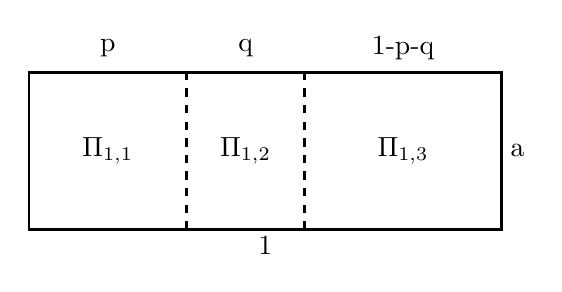
\begin{tikzpicture}[line width=1pt]
        \draw (0,0) rectangle (6,2);
        \draw [dashed](2,0)--(2,2);
        \draw [dashed] (3.5,0)--(3.5,2);
        \node at (3,-0.2) {1};
        \node at (6.2,1){a};
        \node at (1,2.3){p};
        \node at (2.75,2.3){q};
        \node at (4.75,2.3){1-p-q};
        \node at (1,1){$\Pi_{1,1}$};
        \node at (2.75,1){$\Pi_{1,2}$};
        \node at (4.75,1){$\Pi_{1,3}$};
    \end{tikzpicture}
    \caption{}
    \label{21}
\end{figure}

Consider the surface $S(a_0,0,0,p_0,q_0)$.  
  For small $x,y>0$, we let $$\mathbf{R}(x,y)=S(a_0,0,0,p_0-x,q_0-y)\in \Tei_{0,6}.$$ 
  
\begin{Lemma}\label{lemma 4.7}
The family of Riemann surfaces $\{\mathbf{R}(x,y)\}$ is real analytic with respect to the parameters $x$ and $y$.
\end{Lemma}
 \begin{proof}
    We can obtain each
 $\TR(x,y)$ by a quasiconformal deformation of $S(a,0,0,p_0,q_0)$, with Beltrami differential
$\mu(x,y)$  given by $\mu_j(x,y)$ on the annulus $\Pi_{1,j}$ (see Figure \ref{21}),
satisfying 
$$\mu_1(x,y)=\frac{-x}{2p_0-x}, \mu_2(x,y)=\frac{-y}{2q_0-y}, \mu_3(x,y)=\frac{x+y}{2(1-p_0-q_0)+x+y}.$$

 It is obvious that the family of Beltrami differentials  $\{\mu(x,y)\}$ depends real-analytically on $x$ and $y$, so the lemma follows.






 
 %\begin{figure}
     %\centering
     %\includegraphics[width=0.6\linewidth]{1.1.jpg}
     %\caption{}
     %\label{Figure 1.1}
 %\end{figure}

 \end{proof}
 

 
As we have shown, 
 $\TR(x,y)$ depends smoothly on $x$ and $y$, thus $F(\TR(x,y))$ defines a smooth function of $x$ and $y$. 

Now we claim that each $\TR(x,y)$ can be identified  with a certain surface
$$\TS(s,t)=S\left(a(s,t), b(s,t),c(s,t), p(s,t), q(s,t)\right),$$  which arises from 
the  deformation constructed in Section \ref{SCM}. 
We set $p=p_0-x, q=q_0-y$.

\begin{Lemma}\label{lem:locate}
For $x,y$ sufficiently small, we can locate $(s,t)$ such that the surface $$\TS(s,t)=S\left(a(s,t), b(s,t),c(s,t), p(s,t), q(s,t)\right),$$ which is the deformation of the base surface $\TS(0,0)=\TR(x,y)$,
satisfying 
$$p(s,t)=p_0, q(s,t)=q_0.$$
\end{Lemma}
\begin{proof}
By our previous computation, there are positive coefficients $P$ and $Q$ (depending on the base surface $\TR(x,y)$) such that 
\begin{eqnarray*}
\begin{cases}
  p(s,t)-p = \left(P+o(1)\right)  t\ln{\frac{1}{t}}+O(s), \\
 q(s,t)- q = \left(-P+o(1)\right)  t\ln{\frac{1}{t}}+ \left(Q+o(1)\right)  s\ln{\frac{1}{s}}.
\end{cases}
\end{eqnarray*}
We set
 \begin{eqnarray*}
\begin{cases}
 u = s\ln{\frac{1}{s}}, \\
 v = t\ln{\frac{1}{t}}.
\end{cases}
\end{eqnarray*}
Then the value of
 $\left( p(s,t)-p, q(s,t)-q\right)$
is approximately $\left( P v, -P v+ Qu \right)$. Note that the inverse of the matrix $\left[ {\begin{array}{cc}
    0 & P \\
    Q & -P \\
  \end{array} } \right]$ is  $\left[ {\begin{array}{cc}
    \frac{1}{Q} & \frac{1}{Q} \\
    \frac{1}{P} & 0 \\
  \end{array} } \right]$, which is positive. 
Thus for $x,y>0$ that are sufficiently small, there exist  $u>0, v>0$ (and then $s>0, t>0$) such that 
$$ p(s,t)-p=x, \quad q(s,t)-q =y.$$
This gives $p(s,t)=p_0, q(s,t)=q_0$.


\end{proof}


Now we are able to prove Theorem \ref{thm:typeA}. 
Using the same notation as in Lemma \ref{lem:locate}, we have 
 \begin{eqnarray*}
\left[ {\begin{array}{cc}
    x \\
    y \\
  \end{array} } \right] = \left[ {\begin{array}{cc}
    o(1) & P+ o(1)  \\
    Q +o(1) & -P +o(1) \\
  \end{array} } \right]  \left[ {\begin{array}{cc}
    u \\
    v \\
  \end{array} } \right]
\end{eqnarray*} 
   This gives 
      \begin{eqnarray*}
\left[ {\begin{array}{cc}
    u \\
    v \\
  \end{array} } \right] = \left[ {\begin{array}{cc}
    \frac{1}{Q}+o(1) & \frac{1}{Q}+o(1) \\
    \frac{1}{P}+o(1) & o(1) \\
  \end{array} } \right]  \left[ {\begin{array}{cc}
    x \\
    y \\
  \end{array} } \right]
\end{eqnarray*} 
     Recall that $u=s\ln \frac{1}{s}, v= t\ln \frac{1}{t}$.
     Thus $s=\frac{u}{\ln \frac{1}{s}}, t=\frac{v}{\ln \frac{1}{t}}$. 
     Since
     $$\ln{\frac{1}{s}}=(1+o(1))\ln{\frac{1}{u}}, \ln{\frac{1}{t}}=(1+o(1))\ln{\frac{1}{v}},$$
      we have 
       $$s=\frac{u}{(1+o(1))\ln{\frac{1}{u}}},t=\frac{v}{(1+o(1))\ln{\frac{1}{v}}}.$$
    As a consequence, we obtain
    \begin{eqnarray*}
    % \nonumber % Remove numbering (before each equation)
      s &=& \frac{\left( \frac{1}{Q}+o(1)\right) x + \left( \frac{1}{Q}+o(1)\right) y}{\left(1+o(1)\right) \ln \left( \frac{1}{\left( \frac{1}{Q}+o(1)\right) x + \left( \frac{1}{Q}+o(1)\right) y}\right)} \\
      &=& \frac{\frac{x}{Q}+\frac{y}{Q}+o(x)+o(y)}{\ln \left(\frac{Q}{x+y}\right)} \\
      &=& \frac{x+y+o(x)+o(y)}{Q\ln\frac{1}{x+y}},
       \end{eqnarray*} 
      where the last equality holds since 
       $$\lim_{x+y \to 0} \frac{\ln \frac{Q}{x+y}}{\ln  \frac{1}{x+y}}=1.$$
      Similarly, we have  
         \begin{eqnarray*}
         t &=&  \frac{x + o(x)+o(y)}{P \ln \frac{1}{x}}.
    \end{eqnarray*}  
    
  By Proposition \ref{prop:area}, substituting $s$ and $t$ with $x$ and $y$, we  find that  
\begin{eqnarray}\label{equ:area}
% \nonumber % Remove numbering (before each equation)
   && \operatorname{Area}(L(a(s,t),b(s,t),c(s,t),p_0,q_0)) \nonumber \\
   &= & a(0,0)+\beta_1t+\beta_2s+\beta_{11}t^2\ln \frac{1}{t}+\beta_{22}s^2\ln \frac{1}{s} \nonumber\\
    && +o(st\ln \frac{1}{t})+o(t^2\ln \frac{1}{t}) +o(s^2\ln \frac{1}{s}) \nonumber\\
    &=& a(0,0)+\frac{\beta_1}{P} \frac{x+o(x)+o(y)}{\ln \frac{1}{x}} +\frac{\beta_2 }{Q} \frac{x+y+o(x)+o(y)}{\ln \left(\frac{1}{x+y}\right)}  \\
    && + \pi \frac{x^2}{\ln \frac{1}{x}}+\pi \frac{\left(x+y \right)^2}{\ln \frac{1}{x+y}} 
    +o\left(\frac{x^2+xy+y^2}{\ln \left(\frac{1}{x+y}\right)}\right)+o\left(\frac{x^2}{\ln \frac{1}{x}}\right). \nonumber
\end{eqnarray} 
Here we use   $\beta_{11}=\pi P^2$ and $\beta_{22}=\pi Q^2$.

  
  
    
On the other hand, we have   $\TR(x,y)\cong S(a(s,t),b(s,t),c(s,t),p_0,q_0)$ in $\Tei_{0,6}$. By Lemma \ref{Lemma 4.2},  $F(\TR(x,y))$ is the area of 
    $L\left(a(s,t),b(s,t),c(s,t),p_0,q_0)\right)$.
Note that  $a_0=a(0,0)$ and so $F(S(a_0,0,0,p_0,q_0))=a(0,0)$.
It turns out that \eqref{equ:area} is exactly the value of the function $F(\TR(x,y))$.

Since $F(\TR(x,y))$ is smooth, so is $\eqref{equ:area}$. Thus, we have 

\begin{eqnarray}\label{equ:taylor}
 &&  \frac{\beta_1}{P} \frac{x+o(x)+o(y)}{\ln \frac{1}{x}} +\frac{\beta_2 }{Q} \frac{x+y+o(x)+o(y)}{\ln \left(\frac{1}{x+y}\right)} \nonumber \\
    && + \pi \frac{x^2}{\ln \frac{1}{x}}+\pi \frac{\left(x+y \right)^2}{\ln \frac{1}{x+y}} 
    +o\left(\frac{x^2+xy+y^2}{\ln \left(\frac{1}{x+y}\right)}\right)+o\left(\frac{x^2}{\ln \frac{1}{x}}\right) \\
   &=& \delta_{1}x +\delta_{2}y + \delta_{11}x^2 + \delta_{12}xy + \delta_{22}y^2+ O\left((x+y)^3\right)\nonumber
\end{eqnarray}
If we take $x\to 0$, then we get 
$$\frac{\beta_2}{Q}\frac{y+o(y)}{\ln \frac{1}{y}}=\delta_2 y + \delta_{22}y^2+O\left(y^3\right).$$
Divide both sides by $y$ and take $y\to 0$, we obtain $\delta_2=0$. So we have 
$$\frac{\beta_2}{Q}\frac{y+o(y)}{\ln \frac{1}{y}}= \delta_{22}y^2+O\left(y^3\right).$$
Now we divide both sides by $y^2$ and take $y\to 0$ to conclude that $\beta_2=0$. 
As a consequence, the equation \eqref{equ:taylor} becomes 
\begin{eqnarray}\label{equ:taylor2}
 &&  \frac{\beta_1}{P} \frac{x+o(x)+o(y)}{\ln \frac{1}{x}} 
    + \pi \frac{x^2}{\ln \frac{1}{x}}+\pi \frac{\left(x+y \right)^2}{\ln \frac{1}{x+y}} \nonumber \\
     && +o\left(\frac{x^2+xy+y^2}{\ln \left(\frac{1}{x+y}\right)}\right)+o\left(\frac{x^2}{\ln \frac{1}{x}}\right) \\
   &=& \delta_{1}x + \delta_{11}x^2 + \delta_{12}xy + \delta_{22}y^2+ O\left((x+y)^3\right)\nonumber
\end{eqnarray}
If we take $y\to 0$, then we get 
\begin{eqnarray*}
 &&  \frac{\beta_1}{P} \frac{x+o(x)}{\ln \frac{1}{x}} 
    + 2\pi \frac{x^2}{\ln \frac{1}{x}}
     +o\left(\frac{x^2}{\ln \left(\frac{1}{x}\right)}\right) \\
   &=& \delta_{1}x + \delta_{11}x^2 + O\left(x^3\right).
\end{eqnarray*}
The same analysis as above shows  $\delta_1=\beta_1=0$. So the equation \eqref{equ:taylor2}
becomes 
\begin{eqnarray*}
 && \pi \frac{x^2}{\ln \frac{1}{x}}+\pi \frac{\left(x+y \right)^2}{\ln \frac{1}{x+y}} \nonumber \\
     && +o\left(\frac{x^2+xy+y^2}{\ln \left(\frac{1}{x+y}\right)}\right)+o\left(\frac{x^2}{\ln \frac{1}{x}}\right) \\
   &=&  \delta_{11}x^2 + \delta_{12}xy + \delta_{22}y^2+ O\left((x+y)^3\right)\nonumber
\end{eqnarray*}
By taking $x\to 0$, we deduce that  
\begin{eqnarray*}
 && \pi \frac{y^2}{\ln \frac{1}{y}} +o\left(\frac{y^2}{\ln \left(\frac{1}{y}\right)}\right) \\
   &=&  \delta_{22}y^2+ O\left(y^3\right).
\end{eqnarray*}
If we divide both sides  by $y^2/\ln \frac{1}{y}$, then we obtain $\delta_{22}=0$,
which is impossible. 


%And if we  take  $y\to 0$ and let $x$ be small enough, then we can get $\beta_1=0$. 
%It follows that 
%\begin{eqnarray*}\label{equ:area2}
%&& %\beta_{12} \frac{\frac{1}{P_1^2Q_2}x^2+\frac{xy}{P_1Q_2}}{\ln \left(\frac{1}{\frac{Q_1x}{P_1Q_2}+\frac{y}{Q_2}}\right)}  + 
%\frac{\beta_{11}}{P^2} \frac{x^2}{\ln \frac{P}{x}}+\frac{\beta_{22}}{Q^2} \frac{\left(x+y\right)^2}{\ln \left(\frac{Q}{x+y}\right)} \nonumber +o\left(\frac{x^2+xy+y^2}{\ln \left(\frac{Q}{x+y}\right)}\right)+o\left(\frac{x^2}{\ln \frac{P}{x}}\right) \nonumber \\
 %   &=& \delta_{11}x^2 + 2\delta_{12}xy + \delta_{22}y^2+O\left((x+y)^3\right). 
%\end{eqnarray*} 

%Now if we make $x\to 0$ and let $y$ be small enough, 
% we can get 
% $$\left( \frac{\beta_{22}}{Q^2}+o(1)\right) \frac{y^2}{\ln\frac{Q}{y}} = \delta_{22} y^2 + O(y^3), $$
%which is impossible because $\beta_{22}/Q^2 >0$. 

This completes the proof of Theorem \ref{thm:typeA}.












\begin{comment}
    

\subsection{Type (B)}
%\subsubsection{Caculation}
\noindent Let $L_{2}(a,b,c,p,q)$ be the polygon as in Figure \ref{fig:L2}.
We assume that $c>b>a>0$ and $0<p,q<1,0<p+q<1$. There are $6$ vertices, denote by
 $P_k, k=1, \cdots,6$, at which the interior angles are $\frac{\pi}{2}$, and there are $2$ vertices, denote by $Q_1,Q_2$, at which the interior angles are $\frac{3\pi}{2}$.


\begin{figure}
    \centering
    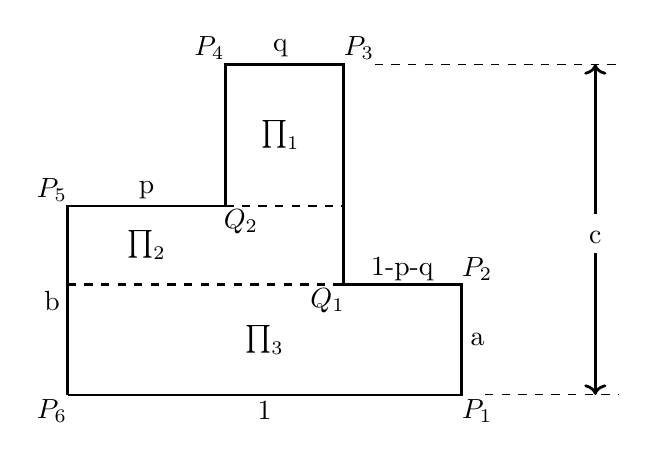
\begin{tikzpicture}[line width=1pt]
        \draw (0,0)--(5,0)--(5,1.4)--(3.5,1.4)--(3.5,4.2)--(2,4.2)--(2,2.4)--(0,2.4)--(0,0);
        \draw[dashed] (2,2.4)--(3.5,2.4);
        \draw[dashed] (0,1.4)--(3.5,1.4);
        \node at (-0.2,-0.2) {$P_6$};
        \node at (5.2,-0.2) {$P_1$};
        \node at (5.2,1.6) {$P_2$};
        \node at (3.7,4.4){$P_3$};
        \node at (3.3,1.2){$Q_1$};
        \node at (1.8,4.4){$P_4$};
        \node at (-0.2,2.6){$P_5$};
        \node at (2.2,2.2){$Q_2$};
        \node at (5.2,0.7){a};
        \node at (-0.2,1.2){b};
        \node at (1,2.6){p};
        \node at (2.7,4.4){q};
        \node at (4.25,1.6){1-p-q};
        \node at(2.5,-0.2){1};
        \node at (2.7,3.3){$\prod_1$};
        \node at (1,1.9){$\prod_2$};
        \node at (2.5,0.7){$\prod_3$};
        \draw [dashed,line width=0.4pt](5.3,0)--(7,0);
        \draw [dashed,line width=0.4pt](3.9,4.2)--  (7,4.2);
        \draw [->] (6.7,2.3)--(6.7,4.2);
        \draw [->] (6.7,1.8)--(6.7,0);
        \node at (6.7,2){c};
    \end{tikzpicture}
    \caption{$L_2(a,b,c,p,q)$}
    \label{fig:L2}
\end{figure}

 Let $S_2(a,b,c,p,q)$ be the double of  $L_2(a,b,c,p,q)$,
  which is considered as a  Riemann sphere with $6$ marked points $P_1, \cdots, P_6$.
Let $\psi_2(a,b,c,p,q)$ be the quadratic differential obtained by 
gluing two copies of $dz^2$ on $L_2(a,b,c,p,q)$. Then $\psi_2(a,b,c,p,q)$ is a Jenkins-Strebel differential with two simple zeros $Q_1, Q_2$. The surface $S_2(a,b,c,p,q)$ is decomposed into three annuli $\Pi_1,\Pi_2,
\Pi_3$, swept out by closed horizontal trajectories of $\psi_2(a,b,c,p,q)$.
This is the quadratic differential that we are going to focus on.

 Fix a polygon $L_2=L_2(a_0,b_0,c_0,p_0,q_0)$. Denote $S_2= S_2(a,b,c,p,q)$ and $\psi_2=\phi_2(a_0,b_0,c_0,p_0,q_0)$. 
The aim of this subsection is to prove 
 \begin{Theorem}\label{thm:typeB}
 The Teichm\"uller disk 
 $\tau^{\psi_2} : \mathbb{H} \to \Tei_{0,6}$ does not admits a holomorphic retraction.  
 \end{Theorem}

  Suppose, towards a contradiction, that $\Phi_2 : \Tei_{0,6} \to \mathbb{H}$ is a holomorphic retraction of $\tau^{\psi_2}$. 
 Let $\mathcal{E}_2:\mathbb{H}^3\rightarrow\Tei_{0,6}$ be the Teichm\"uller polyplane corresponding to $\psi_{2}$. Denote $$b_1=\frac{1}{{\|\psi_{2}\|}_1}\int_{\prod_1}|\psi_{2}|=\frac{(c_0-b_0)q_0}{a_0(1-p_0-q_0)+b_0p_0+c_0q_0},$$
 $$b_2=\frac{1}{{\|\psi_{2}\|}_1}\int_{\prod_2}|\psi_{2}|=\frac{(b_0-a_0)(p_0+q_0)}{a_0(1-p_0-q_0)+b_0p_0+c_0q_0}$$ and
  $$b_3=\frac{1}{{\|\psi_{2}\|}_1}\int_{\prod_3}|\psi_{2}|=\frac{a_0}{a_0(1-p_0-q_0)+b_0p_0+c_0q_0}.$$
By Theorem \ref{thm:GM-JS}, we can assume that $\Phi_2$ satisfies  $$\Phi_2 \circ \mathcal{E}_{2}(\lambda_1,\lambda_2,\lambda_3))=b_1\lambda_1+b_2\lambda_2+b_3\lambda_3$$
for all $(\lambda_1,\lambda_2,\lambda_3)\in \mathbb{H}^3$. 


Note that for any $c>b>a>0$, we have $$\mathcal{E}_{2}\left(\frac{c-b}{c_0-b_0}i,\frac{b-a}{b_0-a_0}i,\frac{a}{a_0}i\right)=S_2(a,b,c,p_0,q_0).$$ 
Thus we have the following equality \begin{equation}\label{equ:linear}
 \Phi_2(S_2(a,b,c,p_0,q_0))=\frac{a(1-p_0-q_0)+bp_0+cq_0}{a_0(1-p_0-q_0)+b_0p_0+c_0q_0}i.
\end{equation}


\begin{Lemma} \label{Lemma 4.11}
Assume that the Teichm\"uller disk 
 $\tau^{\psi_2} : \mathbb{H} \to \Tei_{0,6}$ admits a holomorphic retraction. Then
there exists a holomorphic function $F_2:\Tei_{0,6}\rightarrow \mathbb{H}$ such that $$F_2(S_2(a,b,c,p_0,q_0))=\left( a(1-p_0-q_0)+bp_0+cq_0\right) i$$ for every $c\geq b\geq a>0$.
\end{Lemma}

\begin{proof}
We take 
 $$F_2=\left( a_0(1-p_0-q_0)+b_0p_0+c_0q_0\right) \Phi_2,$$ which is a holomorphic function on $\Tei_{0,6}$. 
 By \eqref{equ:linear}, we have 
 $$F_2(S_2(a,b,c,p_0,q_0))=\left( a(1-p_0-q_0)+bp_0+cq_0\right) i$$ for any $c > b> a>0$.
By continuity, the above equality holds for every $c \geq b\geq a>0$.
\end{proof}













%\begin{figure}
    %\centering
    %\includegraphics[width=0.8\linewidth]{8.jpg}
    %\caption{$L_2(a,b,c,p,q)$}
    %\label{fig:enter-label}
%\end{figure}








\subsection*{The Schwarz-Christoffel maps.}
By the Riemann mapping Theorem, there is a unique conformal map $f$ maps $\mathbb{H}$ to $L_2(a,b,c,p,q)$ with $f(-1)=P_1, f(1)=P_5,  f(\infty)=P_6$. Assume 
$f(\xi_1)=P_2, f(\xi_2)=P_3, f(\xi_3)=P_4$ where $-1<\xi_1<\xi_2<\xi_3<1$. We allow $b=c$ , $a=b$ and assume that 
$f(\eta_1)=Q_1, f(\eta_2)=Q_2$ where $-1<\xi_1<\eta_1\leq\xi_2<\xi_3\leq\eta_2<1$. 
We note that $a=b=c$ iff $\eta_1=\xi_2$ and  $\eta_2=\xi_3$. By  the Schwarz-Christoffel formular, $f$ is given by $$f(z)=J^{-1}\int_0^z\frac{\sqrt{w-\eta_1}\sqrt{w-\eta_2}}{\sqrt{w-\xi_1}\sqrt{w-\xi_2}\sqrt{w-\xi_3}\sqrt{w-1}\sqrt{w+1}}dw.$$

Since $|P_6P_1|=1$, we can have $$J=\int_{-\infty}^{-1}\frac{\sqrt{x-\eta_1}\sqrt{x-\eta_2}}{\sqrt{x-\xi_1}\sqrt{x-\xi_2}\sqrt{x-\xi_3}\sqrt{x-1}\sqrt{x+1}}dx.$$

Since $S_2(a,b,c,p,q)$ is the double of the polygon $L_2(a,b,c,p,q)$, we can extend $f$ to a conformal mapping $$f: \mathbb{C}\setminus
\{-1,\xi_1,\xi_2,\xi_3,1\}\rightarrow S_2(a,b,c,p,q).$$ 





%Our goal is to compute $a(s,t), b(s,t), c(s,t), p(s,t), q(s,t)$.
%Let \begin{eqnarray*}
% \nonumber % Remove numbering (before each equation)A(s,t)=-i\int_{-\infty}^{-1}\frac{\sqrt{x-\xi_1+s}\sqrt{x-\xi_2+t}}{\sqrt{x-1}\sqrt{x+1}\sqrt{x-\xi_1}\sqrt{x-\xi_2}\sqrt{x-\xi_3}}dx,$$
%B(s,t)&=&-i\int_{\xi_1-s}^{\xi_1}\frac{\sqrt{x-\xi_1+s}\sqrt{x-\xi_2+t}}{\sqrt{x-1}\sqrt{x+1}\sqrt{x-\xi_1}\sqrt{x-\xi_2}\sqrt{x-\xi_3}}dx,\\
%C(s,t)&=&-i\int_{\xi_2-t}^{\xi_2}\frac{\sqrt{x-\xi_1+s}\sqrt{x-\xi_2+t}}{\sqrt{x-1}\sqrt{x+1}\sqrt{x-\xi_1}\sqrt{x-\xi_2}\sqrt{x-\xi_3}}dx,\\
%P(s,t)&=&-\int_{\xi_2}^{\xi_3}\frac{\sqrt{x-\xi_1+s}\sqrt{x-\xi_2+t}}{\sqrt{x-1}\sqrt{x+1}\sqrt{x-\xi_1}\sqrt{x-\xi_2}\sqrt{x-\xi_3}}dx,\\
%Q(s,t)&=&-\int_{\xi_1}^{\xi_2-t}\frac{\sqrt{x-\xi_1+s}\sqrt{x-\xi_2+t}}{\sqrt{x-1}\sqrt{x+1}\sqrt{x-\xi_1}\sqrt{x-\xi_2}\sqrt{x-\xi_3}}dx,\\
%J(s,t)&=&\int_{1}^{+\infty}\frac{\sqrt{x-\xi_1+s}\sqrt{x-\xi_2+t}}{\sqrt{x-1}\sqrt{x+1}\sqrt{x-\xi_1}\sqrt{x-\xi_2}\sqrt{x-\xi_3}}dx.\\
%\end{eqnarray*}
%It follows by definition that
%\begin{eqnarray*}
% \nonumber % Remove numbering (before each equation)
  %a(s,t) = \frac{A(s,t)}{J(s,t)}, && 
  %b(s,t) = \frac{B(s,t)}{J(s,t)}, \ \ \ \ 
  %c(s,t) = \frac{C(s,t)}{J(s,t)}, \\
% p(s,t) = \frac{P(s,t)}{J(s,t)}, &&   q(s,t)  = \frac{Q(s,t)}{J(s,t)}.\\
%\end{eqnarray*}

%Both $J(s,t)$ and $A(s,t)$ are real analytic for $s,t \geq 0$ sufficiently small,
% since their integrands depend analytically on $s,t$ and are uniformly integrable. For the other functions, we need more estimates.




\subsection*{Computing the Schwarz-Christoffel maps.}

Fix $-1<\xi_1<\eta_1=\xi_2<\xi_3=\eta_2<1$. 
 Under the Schwarz-Christoffel map,  the corresponding polygon is $L_2(a,a,a,p,q)$. Now
for each pair of small $s>0, t>0$, we deform $L_2(a,a,a,p,q)$ into a new polygon $$L_2\left(a(s,t),b(s,t),c(s,t),p(s,t),q(s,t)\right),$$ which is corresponding to
the Schwarz-Christoffel map that 
maps $(\xi_1, \xi_2, \xi_3)$ into $(P_2, P_3, P_4)$ and $(\xi_2-s, \xi_3+t)$ into $(Q_1, Q_2)$.  
In other words, we have $\eta_1=\xi_2-s, \eta_2=\xi_3+t$.

 Note that for all $s\geq 0, t\geq 0$ (that are sufficiently small), the Riemann surface given by the double of $L_2\left(a(s,t),b(s,t),c(s,t),p(s,t),q(s,t)\right)$ is conformal to  $\mathbb{C}\setminus
\{-1,\xi_1,\xi_2,\xi_3,1\}$.
Thus we obtain a two-dimensional family of surfaces
which represent the same element in $\Tei_{0,6}$.

Our goal is to compute $a(s,t), b(s,t), c(s,t), p(s,t), q(s,t)$.





Let \begin{eqnarray*}
A(s,t)&=&-i\int_{-1}^{\xi_1}\frac{\sqrt{x-\xi_2+s}\sqrt{x-\xi_3-t}}{\sqrt{x-1}\sqrt{x+1}\sqrt{x-\xi_1}\sqrt{x-\xi_2}\sqrt{x-\xi_3}}dx,\\
B(s,t)&=&i\int_{1}^{\infty}\frac{\sqrt{x-\xi_2+s}\sqrt{x-\xi_3-t}}{\sqrt{x-1}\sqrt{x+1}\sqrt{x-\xi_1}\sqrt{x-\xi_2}\sqrt{x-\xi_3}}dx,\\
C(s,t)&=&B(s,t)+i\int_{\xi_3}^{\xi_3+t}\frac{\sqrt{x-\xi_2+s}\sqrt{x-\xi_3-t}}{\sqrt{x-1}\sqrt{x+1}\sqrt{x-\xi_1}\sqrt{x-\xi_2}\sqrt{x-\xi_3}}dx,\\
P(s,t)&=&-\int_{\xi_3+t}^{1}\frac{\sqrt{x-\xi_2+s}\sqrt{x-\xi_3-t}}{\sqrt{x-1}\sqrt{x+1}\sqrt{x-\xi_1}\sqrt{x-\xi_2}\sqrt{x-\xi_3}}dx,\\
Q(s,t)&=&-\int_{\xi_2}^{\xi_3}\frac{\sqrt{x-\xi_2+s}\sqrt{x-\xi_3-t}}{\sqrt{x-1}\sqrt{x+1}\sqrt{x-\xi_1}\sqrt{x-\xi_2}\sqrt{x-\xi_3}}dx,\\
J(s,t)&=&\int_{-\infty}^{-1}\frac{\sqrt{x-\xi_2+s}\sqrt{x-\xi_3-t}}{\sqrt{x-1}\sqrt{x+1}\sqrt{x-\xi_1}\sqrt{x-\xi_2}\sqrt{x-\xi_3}}dx.\\
\end{eqnarray*}

It follows by definition that
\begin{eqnarray*}
% \nonumber % Remove numbering (before each equation)
  a(s,t) = \frac{A(s,t)}{J(s,t)}, && 
  b(s,t) = \frac{B(s,t)}{J(s,t)}, \ \ \ \ 
  c(s,t) = \frac{C(s,t)}{J(s,t)}, \\
 p(s,t) = \frac{P(s,t)}{J(s,t)}, &&   q(s,t)  = \frac{Q(s,t)}{J(s,t)}.\\
\end{eqnarray*}

 $J(s,t)$, $A(s,t)$ and $B(s,t)$ are real analytic for $s,t \geq 0$ sufficiently small,
 since their integrands depend analytically on $s,t$ and are uniformly integrable. For the other functions, we need more estimates.



\begin{Proposition}
    We have $$C(s,t)=B(0,0)+C_1t+C_2s+o(t)+o(s).$$
\end{Proposition}
\begin{proof}
 Firstly, $B(s,t)$ is analytic about $s$ and $t$.
Suppose $B(s,t)=B(0,0)+B_1t +B_2s +o(s)+o(t)+O(st)$.
      Secondly, for small $s,t>0$, we have the equality
   $$\frac{i}{\sqrt{x-1}\sqrt{x+1}\sqrt{x-\xi_1}}=\frac{1+O(t)}{\sqrt{1-\xi_3}\sqrt{\xi_3+1}\sqrt{\xi_3-\xi_1}},$$   
 which holds for every $x\in[\xi_3,\xi_3+t].$ So we have $$C(s,t)=B(0,0)+B_1t +B_2s+\frac{1+O(t)}{\sqrt{1-\xi_3}\sqrt{\xi_3+1}\sqrt{\xi_3-\xi_1}}\int_{\xi_3}^{\xi_3+t}\frac{\sqrt{x-\xi_2+s}\sqrt{x-\xi_3-t}}{\sqrt{x-\xi_2}\sqrt{x-\xi_3}}dx.$$  
 Since $$\int_{\xi_3}^{\xi_3+t}\frac{\sqrt{x-\xi_2+s}\sqrt{x-\xi_3-t}}{\sqrt{x-\xi_2}\sqrt{x-\xi_3}}dx\asymp\int_{\xi_3}^{\xi_3+t}\frac{\sqrt{x-\xi_3-t}}{\sqrt{x-\xi_3}}dx,$$ it suffices to compute integral in the right-hand side. Substituting $x-\xi_3=y$ then yields 
 \begin{eqnarray*}
 \int_{\xi_3}^{\xi_3+t}\frac{\sqrt{x-\xi_3-t}}{\sqrt{x-\xi_3}}dx&=&i\int_0^t\frac{\sqrt{t-y}}{\sqrt{y}}dy\\&=&i[\sqrt{t-y}\sqrt{y}+t\arctan(\frac{\sqrt{y}}{\sqrt{t-y}})]|_0^t=i\frac{t\pi}{2}.
\end{eqnarray*}
      %we have 
      %\begin{align*}
          %\int_{\xi_3}^{\xi_3+m}\frac{\sqrt{x-\xi_2+s}\sqrt{x-\xi_3-m}}{\sqrt{x-1}\sqrt{x+1}\sqrt{x-\xi_1}\sqrt{x-\xi_2}\sqrt{x-\xi_3}}dx&\asymp^*\frac{-i\int_{\xi_3}^{\xi_3+m}\frac{\sqrt{x-\xi_3-m}}{\sqrt{x-\xi_3}}dx}{\sqrt{1-\xi_3}\sqrt{1+\xi_3}\sqrt{\xi_3-\xi_1}}\\&=\frac{\int_0^m\frac{\sqrt{m-z}}{\sqrt{z}}dz}{\sqrt{1-\xi_3}\sqrt{1+\xi_3}\sqrt{\xi_3-\xi_1}}\\&=\frac{\pi m}{2\sqrt{1-\xi_3}\sqrt{1+\xi_3}\sqrt{\xi_3-\xi_1}}
      %\end{align*}
      Combine these two conclusions, we can get
      $$C_1=B_1+\frac{i\pi}{2\sqrt{1-\xi_3}\sqrt{\xi_3+1}\sqrt{\xi_3-\xi_1}}$$
 \end{proof}  
 \begin{Remark}\label{Rem}
We have $$C_1-B_1=\frac{i\pi }{2\sqrt{1-\xi_3}\sqrt{1+\xi_3}\sqrt{\xi_3-\xi_1}}\neq0.$$
\end{Remark}
\begin{Proposition}
    We have $$P(s,t)-P(0,0)=\frac{-i}{2\sqrt{1-\xi_3}\sqrt{\xi_3+1}\sqrt{\xi_3-\xi_1}}t\ln{\frac{1}{t}}+o(t\ln{\frac{1}{t}})+O(s).$$ 
\end{Proposition}   



\begin{proof}
    

  We have
\begin{eqnarray}\label{equ2 P}
 \nonumber   P(s,t)-P(0,0)&=&\int_{\xi_3}^{\xi_3+t}\frac{1}{\sqrt{x-1}\sqrt{x+1}\sqrt{x-\xi_1}}dx\\
    &&+\int_{\xi_3+t}^1\frac{1}{\sqrt{x-1}\sqrt{x+1}\sqrt{x-\xi_1}}\left(1-\frac{\sqrt{x-\xi_2+s}\sqrt{x-\xi_3-t}}{\sqrt{x-\xi_2}\sqrt{x-\xi_3}}\right)dx 
\end{eqnarray}
Firstly, for the first term of (\ref{equ2 P}), we have $$\int_{\xi_3}^{\xi_3+t}\frac{1}{\sqrt{x-1}\sqrt{x+1}\sqrt{x-\xi_1}}dx=O(t).$$ 

Secondly,  we compute the second term. Denote 
$$h(x)=\frac{1}{\sqrt{x-1}\sqrt{x+1}\sqrt{x-\xi_1}},$$ 
which is negative when $\xi_3+t<x<1.$
We write the second term in (\ref{equ2 P}) as 
\begin{eqnarray}\label{equ2 P2}
  \nonumber&&\int_{\xi_3+t}^1 h(x)\left(1-\frac{\sqrt{x-\xi_2+s}\sqrt{x-\xi_3-t}}{\sqrt{x-\xi_2}\sqrt{x-\xi_3}}\right)dx\\&=&\int_{\xi_3+t}^1 h(x)\left(1-\frac{\sqrt{x-\xi_2+s}}{\sqrt{x-\xi_2}}\right)dx+\int_{\xi_3+t}^1
  h(x)\frac{\sqrt{x-\xi_2+s}}{\sqrt{x-\xi_2}}\left(1-\frac{\sqrt{x-\xi_3-t}}{\sqrt{x-\xi_3}}\right)dx
\end{eqnarray}
Obviously, the first term is $O(t)+O(s).$
Thus we only need to estimate the second term in (\ref{equ2 P2}). We suppose n=100.
\begin{eqnarray}
   \nonumber &&\int_{\xi_3+t}^1
  h(x)\frac{\sqrt{x-\xi_2+s}}{\sqrt{x-\xi_2}}\left(1-\frac{\sqrt{x-\xi_3-t}}{\sqrt{x-\xi_3}}\right)dx\\  &\asymp&\int_{\xi_3+t}^1
  h(x)\left(1-\frac{\sqrt{x-\xi_3-t}}{\sqrt{x-\xi_3}}\right)dx\\ \nonumber&=&\int_{\xi_3+t}^{\xi_3+nt}
  h(x)\left(1-\frac{\sqrt{x-\xi_3-t}}{\sqrt{x-\xi_3}}\right)dx
  \nonumber +\int_{\xi_3+nt}^{1}
  h(x)\left(1-\frac{\sqrt{x-\xi_3-t}}{\sqrt{x-\xi_3}}\right)dx
\end{eqnarray}
Substituting $x-\xi_3=y$, we have 
\begin{eqnarray*}
  &&  \int_{\xi_3+t}^1
  h(x)\left(1-\frac{\sqrt{x-\xi_3-t}}{\sqrt{x-\xi_3}}\right)dx\\&=&\int_{t}^{nt}
  h(y+\xi_3)\left(1-\frac{\sqrt{y-t}}{\sqrt{y}}\right)dy
  \nonumber+\int_{nt}^{1-\xi_3}
  h(y+\xi_3)\left(1-\frac{\sqrt{y-t}}{\sqrt{y}}\right)dy\\
  &=&O(t)+\frac{1}{2}\int_{nt}^{1-\xi_3}
  h(y+\xi_3)\left(\frac{t}{y}+O(\frac{t^2}{y^2})\right)dy\\
  &=&\frac{h(\xi_3)}{2}t\ln{\frac{1}{t}}+O(t).
\end{eqnarray*}
Note that $$h(\xi_3)=\frac{-i}{\sqrt{1-\xi_3}\sqrt{\xi_3+1}\sqrt{\xi_3-\xi_1}},$$ we can get the proposition.


%$\int_{\xi_3+m}^1\frac{1}{\sqrt{x-1}\sqrt{x+1}\sqrt{x-\xi_1}}(1-\frac{\sqrt{x-\xi_2+s}\sqrt{x-\xi_3-m}}{\sqrt{x-\xi_2}\sqrt{x-\xi_3}})dx=-C_0i\int_{\xi_3+m}^11-\frac{\sqrt{x-\xi_2+s}\sqrt{x-\xi_3-m}}{\sqrt{x-\xi_2}\sqrt{x-\xi_3}}dx$ for some $C_0>0$. 

%Finally,
%\begin{align*}
    %\int_{\xi_3+m}^11-\frac{\sqrt{x-\xi_2+s}\sqrt{x-\xi_3-m}}{\sqrt{x-\xi_2}\sqrt{x-\xi_3}}dx=&\int_{\xi_3+m}^11-\frac{\sqrt{x-\xi_2+s}}{\sqrt{x-\xi_2}}dx\\+&\int_{\xi_3+m}^1\frac{\sqrt{x-\xi_2+s}}{\sqrt{x-\xi_2}}(1-\frac{\sqrt{x-\xi_3-m}}{\sqrt{x-\xi_3}})dx
%\end{align*}

%\begin{align*}
    %Substituting $x-\xi_2=y$ we have 
%\begin{align*}
%\int_{\xi_3+m}^{1}(1-\frac{\sqrt{x-\xi_2+s}}{\sqrt{x-\xi_2}})dx&=1-\xi_3-m-\int_{\xi_3-\xi_2+m}^{1-\xi_2}\frac{\sqrt{y+s}}{\sqrt{y}}dy\\&=1-\xi_3-m-[\sqrt{y}\sqrt{y+s}+s\log(\sqrt{y}+\sqrt{y+s})]|_{\xi_3-\xi_2+m}^{1-\xi_2}\\&=1-\xi_3-m-\sqrt{1-\xi_2+s}\sqrt{1-\xi_2}\\&+\sqrt{\xi_3-\xi_2+m}\sqrt{\xi_3-\xi_2+m+s}\\&-s\log (\sqrt{1-\xi_2}+\sqrt{1-\xi_2+s})\\&+s\log (\sqrt{\xi_3-\xi_2+m}+\sqrt{\xi_3-\xi_2+m+s})\\&=C_0's+o(s)
%\end{align*}
%\end{align*}
%for some $C_0'>0$.


%Since $\frac{\sqrt{x-\xi_2+s}}{\sqrt{x-\xi_2}}>0$
%when  $\xi_3+m<x<1$,
%\begin{align*}
    %\int_{\xi_3+m}^{1}\frac{\sqrt{x-\xi_2+s}}{\sqrt{x-\xi_2}}(1-\frac{\sqrt{x-\xi_3-m}}{\sqrt{x-\xi_3}})dx=C_0''\int_{\xi_3+m}^{1}(1-\frac{\sqrt{x-\xi_3-m}}{\sqrt{x-\xi_3}})dx
%\end{align*}
%where $C_0''>0$.


%Substituting $x-\xi_3=z$, we have 

%\begin{align*}
%\int_{\xi_3+m}^{1}(1-\frac{\sqrt{x-\xi_3-m}}{\sqrt{x-\xi_3}})dx&=1-\xi_3-m-\int_{m}^{1-\xi_3}\frac{\sqrt{z-m}}{\sqrt{z}}dz\\&=1-\xi_3-m-[\sqrt{z}\sqrt{z-m}-m\log(\sqrt{z}+\sqrt{z-m})]|_{m}^{1-\xi_3}\\&=1-\xi_3-m-\sqrt{1-\xi_3-m}\sqrt{1-\xi_3}\\&+ m\log({\sqrt{1-\xi_3}+\sqrt{1-\xi_3-m}})-m\log{\sqrt{m}} 
%\end{align*}
%Combinating these equalities, we can get the proposition.

\end{proof}

  
      \begin{Proposition}
          There are $Q_1>0,Q_2>0$ such that 
          $$Q(s,t)-Q(0,0)=iQ_1s\ln\frac{1}{s}+iQ_2t\ln\frac{1}{t}+O(st)+o(s\ln\frac{1}{s})+o(t\ln\frac{1}{t}).$$ %holds, where $Q_i(i=1,2)>0$
      \end{Proposition}
      \begin{proof}
          
      
   By the fomula of $Q(s,t)$, we have 
 \begin{eqnarray}\label{eq2 Q}
     Q(s,t)-Q(0,0)=\int_{\xi_2}^{\xi_3}\frac{1}{\sqrt{x-1}\sqrt{x+1}\sqrt{x-\xi_1}}\left(1-\frac{\sqrt{x-\xi_2+s}\sqrt{x-\xi_3-t}}{\sqrt{x-\xi_2}\sqrt{x-\xi_3}}\right)dx%\\&=-\bar{C}i\int_{\xi_2}^{\xi_3}(1-\frac{\sqrt{x-\xi_2+s}\sqrt{x-\xi_3-t}}{\sqrt{x-\xi_2}\sqrt{x-\xi_3}})dx
 \end{eqnarray}
 %where $\bar{C}>0.$
 Denote $$h(x)=\frac{1}{\sqrt{x-1}\sqrt{x+1}\sqrt{x-\xi_1}},$$ which is negative when $\xi_2<x<\xi_3.$
We write (\ref{eq2 Q})  as 
\begin{eqnarray}\label{equ2 Q}
   \nonumber &&\int_{\xi_2}^{\xi_3}h(x)\left(1-\frac{\sqrt{x-\xi_2+s}\sqrt{x-\xi_3-t}}{\sqrt{x-\xi_2}\sqrt{x-\xi_3}}\right)dx\\&=&\int_{\xi_2}^{\xi_3}h(x)\left(1-\frac{\sqrt{x-\xi_2+s}}{\sqrt{x-\xi_2}}\right)dx+\int_{\xi_2}^{\xi_3}h(x)\frac{\sqrt{x-\xi_2+s}}{\sqrt{x-\xi_2}}\left(1-\frac{\sqrt{x-\xi_3-t}}{\sqrt{x-\xi_3}}\right)dx
\end{eqnarray}
 As for the first term in (\ref{equ2 Q}),%let $n$ be sufficiently large fixed number. 
  substituting $x-\xi_2=y$, we can easily get that 
 \begin{eqnarray*}
    && \int_{\xi_2}^{\xi_3}h(x)\left(1-\frac{\sqrt{x-\xi_2+s}}{\sqrt{x-\xi_2}}\right)dx\\&=&\int_{0}^{\xi_3-\xi_2}h(y+\xi_2)\left(1-\frac{\sqrt{y+s}}{\sqrt{y}}\right)dy\\&=&(h(\xi_2)+o(1))[y-\sqrt{y(y+s)}-s\ln(\sqrt{y}+\sqrt{y+s}]|_{0}^{\xi_3-\xi_2}\\&=&-\frac{1}{2}h(\xi_2)s\ln{\frac{1}{s}}+o(s\ln{\frac{1}{s}})%+\int_{ns}^{\xi_3-\xi_2}h(y+\xi_2)\left(1-\frac{\sqrt{y+s}}{\sqrt{y}}\right)dy
 \end{eqnarray*}
% Secondly, 
 %\begin{align*}
    % \int_{\xi_2}^{\xi_3}(1-\frac{\sqrt{x-\xi_2+s}\sqrt{x-\xi_3-m}}{\sqrt{x-\xi_2}\sqrt{x-\xi_3}})dx=&\int_{\xi_2}^{\xi_3}(1-\frac{\sqrt{x-\xi_2+s}}{\sqrt{x-\xi_2}})dx+\\&\int_{\xi_2}^{\xi_3}\frac{\sqrt{x-\xi_2+s}}{\sqrt{x-\xi_2}}(1-\frac{\sqrt{x-\xi_3-m}}{\sqrt{x-\xi_3}})dx
 %\end{align*}
%We can get 
%\begin{align*}
   % \int_{\xi_2}^{\xi_3}(1-\frac{\sqrt{x-\xi_2+s}}{\sqrt{x-\xi_2}})dx&=(\xi_3-\xi_2)-[\sqrt{x-\xi_2}\sqrt{x-\xi_2+s}]|_{\xi_2}^{\xi_3}\\&-[s\log (\sqrt{x-\xi_2}+\sqrt{s+x-\xi_2})]|_{\xi_2}^{\xi_3}\\&=-\frac{1}{2}s\log s^{-1}+o(s\log s^{-1})
%\end{align*}
For the second term, let $n$ be sufficiently large fixed number, we can assume $n=100$,  we have 
\begin{eqnarray}\label{equ2 Q3}
 &&  \nonumber\int_{\xi_2}^{\xi_3}h(x)\frac{\sqrt{x-\xi_2+s}}{\sqrt{x-\xi_2}}\left(1-\frac{\sqrt{x-\xi_3-t}}{\sqrt{x-\xi_3}}\right)dx\\ &=&\int_{\xi_2}^{\xi_2+ns}h(x)\frac{\sqrt{x-\xi_2+s}}{\sqrt{x-\xi_2}}\left(1-\frac{\sqrt{x-\xi_3-t}}{\sqrt{x-\xi_3}}\right)dx\\ \nonumber&&+\int_{\xi_2+ns}^{\xi_3-nt}h(x)\frac{\sqrt{x-\xi_2+s}}{\sqrt{x-\xi_2}}\left(1-\frac{\sqrt{x-\xi_3-t}}{\sqrt{x-\xi_3}}\right)dx\\ \nonumber&&+\int_{\xi_3-nt}^{\xi_3}h(x)\frac{\sqrt{x-\xi_2+s}}{\sqrt{x-\xi_2}}\left(1-\frac{\sqrt{x-\xi_3-t}}{\sqrt{x-\xi_3}}\right)dx
\end{eqnarray}
As for the first term in (\ref{equ2 Q3}), %let $n$ be sufficiently large fixed number, we can assume n=100, %
we have 
\begin{eqnarray*}
 && \int_{\xi_2}^{\xi_2+ns}h(x)\frac{\sqrt{x-\xi_2+s}}{\sqrt{x-\xi_2}}\left(1-\frac{\sqrt{x-\xi_3-t}}{\sqrt{x-\xi_3}}\right)dx\\&=&\int_{\xi_2}^{\xi_2+ns}h(x)\frac{\sqrt{x-\xi_2+s}}{\sqrt{x-\xi_2}}\frac{t}{(\sqrt{x-\xi_3}+\sqrt{x-\xi_3-t})\sqrt{x-\xi_3}}dx\\&=&-\int_{0}^{ns}h(y+\xi_2)\frac{\sqrt{y+s}}{\sqrt{y}}\frac{t}{(\sqrt{\xi_3-\xi_2-y}+\sqrt{\xi_3-\xi_2-y-t})\sqrt{\xi_3-\xi_2-y}}dy\\&=&-\int_{0}^{ns}(h(\xi_2)+o(1))t\frac{\sqrt{y+s}}{\sqrt{y}}\left(\frac{1}{2(\xi_3-\xi_2)}+o(1)\right)dy\\&=&\left(-\frac{h(\xi_2)}{2(\xi_3-\xi_2)}t+o(t)\right)[\sqrt{y(y+s)}+s\ln(\sqrt{y}+\sqrt{y+s})]|_0^{ns}\\&=&-\frac{h(\xi_2)(\sqrt{n(n+1)}+\ln({\sqrt{n}+\sqrt{n+1}}))}{2(\xi_3-\xi_2)}st+o(st)
  \\%\\&=\int_{\xi_2}^{\xi_2+ns}\frac{\sqrt{x-\xi_2+s}}{\sqrt{x-\xi_2}}\left(mdx\\&=\bar{C}''ms+o(sm)
\end{eqnarray*}
%Since $$\frac{t}{(\sqrt{x-\xi_3}+\sqrt{x-\xi_3-t})\sqrt{x-\xi_3}}=$$
%for some $\bar{C}',\bar{C}''\neq0 .$
For the second term in (\ref{equ2 Q3}), substituting $\xi_3-x=z$, we write 








\begin{eqnarray*}
  &&\int_{\xi_2+ns}^{\xi_3-nt}h(x)\frac{\sqrt{x-\xi_2+s}}{\sqrt{x-\xi_2}}\left(1-\frac{\sqrt{x-\xi_3-t}}{\sqrt{x-\xi_3}}\right)dx\\&=&\int_{nt}^{\xi_3-\xi_2-ns}h(\xi_3-z)\frac{\sqrt{\xi_3-z-\xi_2+s}}{\sqrt{\xi_3-z-\xi_2}}\left(1-\frac{\sqrt{z+t}}{\sqrt{z}}\right)dz\\&=&\int_{nt}^{\xi_3-\xi_2-ns}(h(\xi_3)+o(1))\sqrt{1+\frac{s}{\xi_3-z-\xi_2}}\left(1-\sqrt{1+\frac{t}{z}}\right)dz\\&=&(1+O(\frac{1}{n}))\int_{nt}^{\xi_3-\xi_2-ns}(h(\xi_3)+o(1))\left(-\frac{t}{2z}+o(\frac{t}{z})\right)dz
\end{eqnarray*}
%for some $\bar{C}''',\bar{C}''''>0



Applying integration by parts, we obtain 
$$\int_{nt}^{\xi_3-\xi_2-ns}(h(\xi_3)+o(1))\left(-\frac{t}{2z}+o(\frac{t}{z})\right)dz=-\frac{1}{2}h(\xi_3)t\ln{\frac{1}{t}}+o\left(t\ln{\frac{1}{t}}\right).$$

Now we compute the third term in (\ref{equ2 Q3}),



\begin{eqnarray*}
  &&\int_{\xi_3-nt}^{\xi_3}\frac{\sqrt{x-\xi_2+s}}{\sqrt{x-\xi_2}}\left(1-\frac{\sqrt{x-\xi_3-t}}{\sqrt{x-\xi_3}}\right)dx\\&\asymp&\int_{\xi_3-nt}^{\xi_3}1-\frac{\sqrt{x-\xi_3-t}}{\sqrt{x-\xi_3}}dx\\&=&\int_{0}^{nt}1-\frac{\sqrt{z+t}}{\sqrt{z}}dx\\&=&\left(-\frac{n}{n+\sqrt{n(n+1)}}+\ln{\frac{1}{\sqrt{n}+\sqrt{n+1}}}\right)t.
\end{eqnarray*}
%for some $\bar{\bar{C}}>0.$
The proposition follows, by taking 
$$Q_1=\frac{1}{2\sqrt{1-\xi_2}\sqrt{1+\xi_2}\sqrt{\xi_2-\xi_1}},Q_2=\frac{1}{2\sqrt{1-\xi_3}\sqrt{1+\xi_3}\sqrt{\xi_3-\xi_1}}.$$

\end{proof}
\begin{Proposition}
    There exists $\beta_1, \beta_2, \beta_{12},\beta_{11},\beta_{21},\beta_{22}$ such that
\begin{eqnarray*}
&&Area(L_2(a(s,t),b(s,t),c(s,t),p(s,t),q(s,t)))\\&=&a(0,0)+\beta_1t+\beta_2s+\beta_{12}st\ln\frac{1}{t}+\beta_{11}t^2\ln\frac{1}{t}\\&&+\beta_{21}st\ln\frac{1}{s}+\beta_{22}s^2\ln\frac{1}{s}+o(s^2\ln\frac{1}{s})\\&&+o(t^2\ln\frac{1}{t})+o(st\ln\frac{1}{t})+o(st\ln\frac{1}{s})
\end{eqnarray*} holds, where $\beta_{12},\beta_{11},\beta_{21},\beta_{22}$ are not equal to 0 together.
\end{Proposition}
\begin{proof}
We know $J(0,0)=Ji$, where $J>0$. 

Thus we can assume
$$a(s,t)=a(0,0)+A_1t+A_2s+o(t)+o(s);$$ $$b(s,t)=a(0,0)+B_1't+B_2's+o(t)+o(s);$$
$$c(s,t)=a(0,0)+C_1't+C_2's+o(t)+o(s);$$
$$p(s,t)=p(0,0)-P_1t\ln\frac{1}{t}+o(t\ln\frac{1}{t})+O(s);$$
$$q(s,t)=q(0,0)+Q_1't\ln\frac{1}{t}+Q_2's\ln\frac{1}{s}+O(st)+o(t\ln\frac{1}{t})+o(s\ln\frac{1}{s}),$$ where $P_1,Q_1'$ and $Q_2'$ are positive.

This gives the desired equality.

Thus we have 
\begin{eqnarray*}
\beta_{11}&=&A_1(P_1-Q_1')-B_1'P_1+C_1'Q_1'\\
\beta_{12}&=&A_2(P_1-Q_1')-B_2'P_1+C_2'Q_1'\\
\beta_{21}&=&-A_1Q_2'+C_1'Q_2'\\
\beta_{22}&=&-A_2Q_2'+C_2'Q_2'
\end{eqnarray*}


If $\beta_{11}=\beta_{12}=\beta_{21}=\beta_{22}=0$, after some caculations, we have $$A_1=C_1'=B_1', A_2=B_2'=C_2'.$$

However $B_1'=\frac{B_1}{J(0,0)}$ and $C_1'=\frac{C_1}{J(0,0)}$ by Remark\ref{Rem}. It follows that $B_1'\neq C_1'$, which gives the contradiction.
\end{proof}
The Kobayashi metric and the Carath\'{e}odory metric on $S_2(a,b,c,p,q).$

  Fix $S_2(a,a,a,p,q)$ for some $a,p,q$. For small $x,y>0$, we let $S_2(x,y)=S_2(a,a,a,p+x,q-y-\frac{Q_1'}{P_1}x)$. Next we show that $\{S_2(x,y)\}$ is infinitely differentiable about $x$ and $y$ in $\Tei_{0,6}$. We want to show $F_2$ from Lemma\ref{Lemma 4.11} is not smooth along $\{S_2(x,y)\}$ at $(x,y)=(0,0)$. It follows that the Kobayashi metric and the Carath\'{e}odory metric do not agree on $\tau^{\phi_2(a,b,c,p,q)}$.
  
 
\begin{Lemma}
 $S_2(x,y)$ is infinitely differentiable about $x$ and $y$.
\end{Lemma}
 \begin{proof}
 $S_2(x,y)$ can be defined as $S_2(x,y)=[\mu^{(2)}(x,y)]$, where $\mu^{(2)}(x,y)\in BD(S)$ is equal to $\mu^{(2)}_j(x,y)$ on annuli $\prod^{(2)}_j$(see Figure\ref{Fig 23}):

\begin{figure}
    \centering
    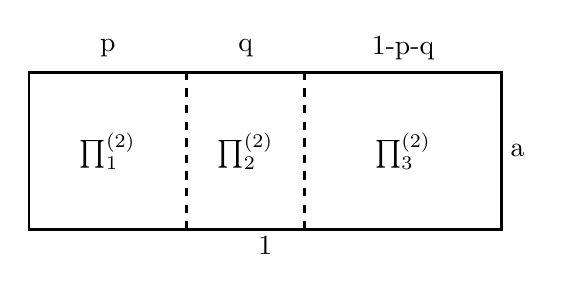
\begin{tikzpicture}[line width=1pt]
        \draw (0,0) rectangle (6,2);
        \draw [dashed](2,0)--(2,2);
        \draw [dashed] (3.5,0)--(3.5,2);
        \node at (3,-0.2) {1};
        \node at (6.2,1){a};
        \node at (1,2.3){p};
        \node at (2.75,2.3){q};
        \node at (4.75,2.3){1-p-q};
        \node at (1,1){$\prod_1^{(2)}$};
        \node at (2.75,1){$\prod_2^{(2)}$};
        \node at (4.75,1){$\prod_3^{(2)}$};
    \end{tikzpicture}
    \caption{}
    \label{Fig 23}
\end{figure}




 
 %\begin{figure}
     %\centering
     %\includegraphics[width=0.6\linewidth]{2.1.jpg}
    % \caption{Caption}
     %\label{fig:enter-label}
% \end{figure}
 $$\mu^{(2)}_1(x,y)=\frac{x}{2p+x}, \mu^{(2)}_2(x,y)=\frac{-y-\frac{Q_1'}{P_1}x}{2q-y-\frac{Q_1'}{P_1}x}, \mu^{(2)}_3(x,y)=\frac{y-x+\frac{Q_1'}{P_1}x}{2(1-p-q)-x+y+\frac{Q_1'}{P_1}x}$$
 \end{proof}
Assume that the Carath\'{e}odory and Kobayashi metrics agree on the disk $\tau^{\phi_2(a,b,c,p,q)}$, for some choice of $a,b,c>0$. Let $F_2:\Tei_{0,6}\rightarrow \mathbb{H}$ be the function from Lemma \ref{Lemma 4.11}
 corresponding to $p$ and $q$.
 
The function $F_2$ is holomorphic and $S_2(x,y)$ is infinitely differentiable about $x$ and $y$, so the function $F_2(S_2(x,y))$ is a complex-valued smooth function of $x$ and $y$. Thus $$F_2(S_2(x,y))=F_2(S_2(0,0))+\delta_1x+\delta_2y+\delta_{11}x^2+\delta_{12}xy+\delta_{22}y^2+O((x+y)^3).$$

By the above, we have the following Lemma:

\begin{Lemma}
Let $a,q,q_1,p,p_1$ be such that $q>q_1,p<p_1$, and denote by $\phi_2$ the holomorphic function from Lemma 5.9 corresponding to $p$ and $q$.There exsit $M_1, M_2, M_{11}, M_{12},M_{22},M_{21}$  where $M_{ij}(i,j=1,2)$ are not all 0 such that

\begin{align*}
\phi_2(S_2(a,a,a,p_1,q_1))=&\phi_2(S_2(a,a,a,p,q))+M_1\frac{t}{\log t^{-1}}+M_2\frac{h}{\log h^{-1}}+\\& M_{11}\frac{t^2}{\log t^{-1}}+M_{22}\frac{h^2}{\log h^{-1}}+M_{12}\frac{th}{\log t^{-1}}+M_{21}\frac{th}{\log h^{-1}}+\\&o(\frac{th}{\log h^{-1}}+\frac{t^2}{\log t^{-1}}+\frac{h^2}{\log h^{-1}}+\frac{th}{\log t^{-1}})    
\end{align*}
where $t=p_1-p, h+\frac{q_1'}{p_1'}t=q-q_1$.
\end{Lemma}

Proof: Given $a,p_1$ and $q_1$, we find $-1<\xi_1<\xi_2<\xi_3<1$ such that the Schwarz-Christoffel map $f=f(\xi_3,\xi_3,\xi_2,\xi_2,\xi_1)$ maps $\mathbb{H}$ onto $S_2(a,a,a,p_1,q_1)$. We consider $S_2(a(m,s),b(m,s),c(m,s),p(m,s),q(m,s))$. Observe that $p(m,s)$ is decrease with $m$ and $q(m,s)$ is increase with $m$ and $s$.

We locate the time $m,s$ such that $p=p(m,s)$ and $q=q(m,s)$.
That are $$p_1-p=t=p_1'm\log m^{-1}+o(m\log m^{-1})+O(s)$$
    $$q-q_1=h+\frac{q_1'}{p_1'}t=q_1'm\log m^{-1}+q_2's\log s^{-1}+O(ms)+o(s\log s^{-1})+o(m\log m^{-1}). $$ for some $q_1'>0,p_1'>0,q_2'>0$.
    Thus we obtain $$m=\frac{(1+o(1))t}{p_1'\log t^{-1}},\log m^{-1}=(1+o(1))\log t^{-1}$$ and $$s=\frac{(1+o(1))h}{q_2'\log {h^{-1}}},\log s^{-1}=(1+o(1))\log h^{-1}.$$ 

    Since by construction $S_2(a,a,a,p_1,q_1)=S_2(a(m,s),b(m,s),c(m,s),p(m,s),q(m,s))$ in $\tau_{0,6}$. By Lemma 5.9  we find that 
    \begin{align*}
        \phi_2(S_2(a,a,a,p_1,q_1))&=\phi_2(S_2(a(m,s),b(m,s),c(m,s),p(m,s),q(m,s)))\\&=iArea(L_2(a(m,s),b(m,s),c(m,s),p(m,s),q(m,s)))
    \end{align*}
On the other hand, we have $a=a(0,0)$ and so $\phi_2(S_2(a(0,0),a,a,p,q)=a(0,0)$.
It follows that 
\begin{align*}
    \phi_2(S_2(a,a,a,p_1,q_1))-\phi_2(S_2(a(0,0),a,a,p,q)=&i[a(m,s)(1-p(m,s)-q(m,s))\\&+b(m,s)p(m,s)+c(m,s)q(m,s)-a(0,0)]
\end{align*}


By Proposition 5.13, replacing $m$ and $s$ with $t$ and $h$, we can get the desired equality.

\begin{Theorem}
    The Carath\'{e}odory metric and Kobayashi metric are not agree on the Teichm\"{u}ller disk $\tau^{\phi_2(a,b,c,p,q)}$ for any choices of $a,b,c,p,q$.
\end{Theorem}
Proof: Suppose not. By Lemma 5.14 and Lemma 5.15, we have 
\begin{align*}
  \delta_1t+\delta_2h+\delta_{11}t^2+\delta_{12}th+\delta_{22}h^2+O((t+h)^3)=&M_1\frac{t}{\log t^{-1}}+M_2\frac{h}{\log h^{-1}}+\\& M_{11}\frac{t^2}{\log t^{-1}}+M_{22}\frac{h^2}{\log h^{-1}}+\\&M_{12}\frac{th}{\log t^{-1}}+M_{21}\frac{th}{\log h^{-1}}+\\&o(\frac{t^2}{\log t^{-1}}+\frac{h^2}{\log h^{-1}})+ \\& o( \frac{th}{\log h^{-1}}+  \frac{th}{\log t^{-1}})
\end{align*}
 Firstly, we make $h=0$ and let $t\rightarrow0$. We can get $\delta_1=0$ and $M_1=0$. Secondly,  we make $t=0$ and let $h\rightarrow0$,we can get $\delta_2=0$ and $M_2=0$.  Thirdly, let $t=0$ again and let $h\rightarrow0$,
 we have $\delta_{22}=0$ and $M_{22}=0$. Let $h=0$ again and $t\rightarrow0$, we can get $\delta_{11}=0$ and $M_{11}=0$.
Thus $\delta_{12}th+O((t+h)^3)=M_{12}\frac{th}{\log t^{-1}}+M_{21}\frac{th}{\log h^{-1}}+o(\frac{t^2}{\log t^{-1}}+\frac{h^2}{\log h^{-1}})$.
Let $h=t$ .
Dividing both two sides of the above equality by $\frac{t^2}{\log (t)^{-1}}$, we get 
 $$\delta_{12}\log t^{-1}+O(t\log t^{-1})=M_{12}+   M_{21}+o(1).$$ Let $t\rightarrow0$, we must have $\delta_{12}=M_{12}+ M_{21}=0$.
Let $h=t^2$ .
Dividing both two sides of the above equality by $\frac{t^2}{\log (t)^{-1}}$, we get 
 $$O(t\log t^{-1})=M_{12}+ M_{21}\frac{t}{2}+o(1).$$ Let $t\rightarrow0$, we must have $M_{12}=M_{21}=0$, which contradicts to Lemma 5.15.
 
 
 






%%%%%%%%%%%%%%%%%%%%%%%%%%%%%%%%%%%%%%%%%%%%%%%%%%%%%%%%%%%%%%%%%%%%%%%%%%%%5


\subsection{Type(C)}
%\subsubsection{Caculation}



\noindent Let $L_{3}(a,b,c,p,q)$ be the polygon as in Figure \ref{fig:L3}.
We assume that $a>b>0, c>a-b$ and $0<p,q<1,0<p+q<1$. There are $6$ vertices, denote by
 $P_k, k=1, \cdots,6$, at which the interior angles are $\frac{\pi}{2}$, and there are $2$ vertices, denote by $Q_1,Q_2$, at which the interior angles are $\frac{3\pi}{2}$.


\begin{figure}
    \centering
    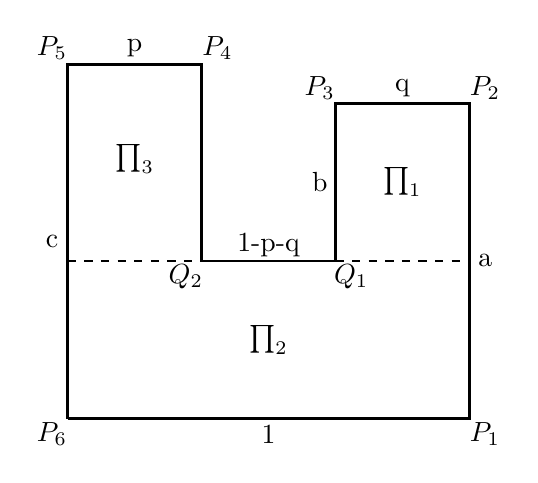
\begin{tikzpicture}[line width=1pt]
        \draw (0,0)--(5.1,0)--(5.1,4)--(3.4,4)--(3.4,2)--(1.7,2)--(1.7,4.5)--(0,4.5)--(0,0);
       \draw [dashed] (3.4,2)--(5.1,2);
        \draw [dashed] (0,2)--(1.7,2);
        \node at (-0.2,-0.2) {$P_6$};
        \node at (5.3,-0.2) {$P_1$};
        \node at (5.3,4.2) {$P_2$};
        \node at (3.2,4.2){$P_3$};
        \node at (1.9,4.7){$P_4$};
        \node at (-0.2,4.7){$P_5$};
        \node at (3.6,1.8) {$Q_1$};
        \node at (1.5,1.8){$Q_2$};
        \node at (2.55,-0.2){1};
        \node at (5.3,2){a};
        \node at (4.25,4.2){q};
        \node at (2.55,2.2){1-p-q};
        \node at (0.85,4.7){p};
        \node at (-0.2,2.25){c};
        \node at (3.2,3){b};
        \node at (2.55,1){$\prod_2$};
        \node at (4.25,3){$\prod_1$};
        \node at (0.85,3.3){$\prod_3$};
    \end{tikzpicture}
    \caption{$L_3(a,b,c,p,q)$}
    \label{fig:L3}
\end{figure}


 Let $S_3(a,b,c,p,q)$ be the double of  $L_3(a,b,c,p,q)$,
  which is considered as a  Riemann sphere with $6$ marked points $P_1, \cdots, P_6$.
Let $\psi_3(a,b,c,p,q)$ be the quadratic differential obtained by 
gluing two copies of $dz^2$ on $L_3(a,b,c,p,q)$. Then $\psi_3(a,b,c,p,q)$ is a Jenkins-Strebel differential with two simple zeros $Q_1, Q_2$. The surface $S_3(a,b,c,p,q)$ is decomposed into three annuli $\Pi_1,\Pi_2,
\Pi_3$, swept out by closed horizontal trajectories of $\psi_3(a,b,c,p,q)$.
This is the quadratic differential that we are going to focus on.

Fix a polygon $L_3=L_3(a_0,b_0,c_0,p_0,q_0)$. Denote $S_3= S_3(a,b,c,p,q)$ and $\psi_3=\phi_3(a_0,b_0,c_0,p_0,q_0)$. 
The aim of this subsection is to prove 
 \begin{Theorem}\label{thm:typeC}
 The Teichm\"uller disk 
 $\tau^{\psi_3} : \mathbb{H} \to \Tei_{0,6}$ does not admits a holomorphic retraction.  
 \end{Theorem}

 Suppose, towards a contradiction, that $\Phi_3 : \Tei_{0,6} \to \mathbb{H}$ is a holomorphic retraction of $\tau^{\psi_3}$. 
 Let $\mathcal{E}_3:\mathbb{H}^3\rightarrow\Tei_{0,6}$ be the Teichm\"uller polyplane corresponding to $\psi_{3}$. Denote  $$c_1=\frac{1}{{\|\psi_{3}\|}_1}\int_{\prod_1}|\psi_{3}|=\frac{b_0q_0}{(a_0-b_0)(1-p_0-q_0)+a_0q_0+c_0p_0},$$
 $$c_2=\frac{1}{{\|\psi_{3}\|}_1}\int_{\prod_2}|\psi_{3}|=\frac{a_0-b_0}{(a_0-b_0)(1-p_0-q_0)+a_0q_0+c_0p_0}$$ and
  $$c_3=\frac{1}{{\|\psi_{3}\|}_1}\int_{\prod_3}|\psi_{3}|=\frac{(c_0-a_0+b_0)p_0}{(a_0-b_0)(1-p_0-q_0)+a_0q_0+c_0p_0}.$$
By Theorem \ref{thm:GM-JS}, we can assume that $\Phi_3$ satisfies  $$\Phi_3 \circ \mathcal{E}_{3}(\lambda_1,\lambda_2,\lambda_3))=c_1\lambda_1+c_2\lambda_2+c_3\lambda_3$$
for all $(\lambda_1,\lambda_2,\lambda_3)\in \mathbb{H}^3$. 


Note that for any $a>b>0,c>a-b$, we have $$\mathcal{E}_{3}\left(\frac{b}{b_0}i,\frac{a-b}{a_0-b_0}i,\frac{c-a+b}{c_0-a_0+b_0}i\right)=S_3(a,b,c,p_0,q_0).$$ 
Thus we have the following equality \begin{equation}\label{equ:linear}
 \Phi_3(S_3(a,b,c,p_0,q_0))=\frac{(a-b)(1-p_0-q_0)+aq_0+cp_0}{(a_0-b_0)(1-p_0-q_0)+a_0q_0+c_0p_0}i.
\end{equation}


\begin{Lemma} Assume that the Teichm\"uller disk 
 $\tau^{\psi_3} : \mathbb{H} \to \Tei_{0,6}$ admits a holomorphic retraction. Then
there exists a holomorphic function $F_3:\Tei_{0,6}\rightarrow \mathbb{H}$ such that $$F_3(S_3(a,b,c,p_0,q_0))=\left((a-b)(1-p_0-q_0)+aq_0+cp_0\right) i$$ for every $a\geq b>0, c\geq a- b$.
\end{Lemma}

\begin{proof}
We take 
 $$F_3=\left( (a_0-b_0)(1-p_0-q_0)+a_0q_0+c_0p_0\right) \Phi_3,$$ which is a holomorphic function on $\Tei_{0,6}$. 
 By \eqref{equ:linear}, we have 
 $$F_3(S_3(a,b,c,p_0,q_0))=\left( (a-b)(1-p_0-q_0)+aq_0+cp_0\right) i$$ for any $a>b>0,c>a-b>0$.
By continuity, the above equality holds for every $a\geq b>0,c \geq a-b$.
\end{proof}








 %Let $S_3=S_3(a,b,c,p,q)$ be the double of the polygon $L_3(a,b,c,p,q)$.
%Then $S_3$ is a six-timess-punctured  Riemann sphere with the mark points $P_k's$. We allow $b=0,c=a$. In this case, $S_3$ is a pillowcase surface with the additional marked point $P_3, P_4,P_2,P_5$ are on the same line.

%The $(2,0)$ form $dz^2$ lives on the polygon $L_3(a,b,c,p,q)$. After doubling, the two copies of the form $dz^2$ glue together along the edges of $L_3(a,b,c,p,q)$ to form the holomorphic quadratic differential $\phi_3=\phi_3(a,b,c,p,q)$ on $S_3$. This differential has first-order poles at the points $P_k$ and first-order zero at $Q_l$. Moreover, $\phi_3$ is a Jenkins-Strebel differential and $S_3$ decomposes into three nondegenerate annuli $\prod_1,\prod_2,
%\prod_3$ swept out by closed horizontal trajectories of $\phi_3$





%\begin{figure}
    %\centering
    %\includegraphics[width=0.7\linewidth]{9.jpg}
    %\caption{$L_3(a,b,c,p,q)$}
    %\label{fig:enter-label}
%\end{figure}


 %Fix $(a_0,b_0,c_0,p_0,q_0)$ and let $\phi_{3,0}=\phi_3(a_0,b_0,c_0,p_0,q_0)$. Let $\epsilon_{3,0}:\mathbb{H}^3\rightarrow\tau_{0,6}$ be the polyplane mapping corresponding to $\phi_{3,0}$. Set $$d_1=\frac{1}{{\|\phi_{3,0}\|}_1}\int_{\prod_1}|\phi_{3,0}|=\frac{b_0q_0}{(a_0-b_0)(1-p_0-q_0)+a_0q_0+c_0p_0},$$
% $$d_2=\frac{1}{{\|\phi_{3,0}\|}_1}\int_{\prod_2}|\phi_{3,0}|=\frac{a_0-b_0}{(a_0-b_0)(1-p_0-q_0)+a_0q_0+c_0p_0}$$ and
  %$$d_3=\frac{1}{{\|\phi_{3,0}\|}_1}\int_{\prod_3}|\phi_{3,0}|=\frac{(c_0-a_0+b_0)p_0}{(a_0-b_0)(1-p_0-q_0)+a_0q_0+c_0p_0}.$$
  %If $\tau^{\phi_{3,0}}$ is a extremal disk, then by Theorem 3.2 there exists a holomorphic map $\Phi_3:\tau_{0,6}\rightarrow \mathbb{H}$ such that $$\Phi_3(\epsilon_{3,0}(\lambda_1,\lambda_2,\lambda_3))=d_1\lambda_1+d_2\lambda_2+d_3\lambda_3.$$
%where $(\lambda_1,\lambda_2,\lambda_3)\in \mathbb{H}^3$. We can find that for any $a,b,c$ such that $$\epsilon_{3,0}(\frac{b}{b_0}i,\frac{a-b}{a_0-b_0}i,\frac{c-a+b}{c_0-a_0+b_0}i)=S_3(a,b,c,p_0,q_0)$$ holds. Thus we get the equality $$\Phi_3(S_3(a,b,c,p_0,q_0))=\frac{(a-b)(1-p_0-q_0)+aq_0+cp_0}{(a_0-b_0)(1-p_0-q_0)+a_0q_0+c_0p_0}i.$$
%Thus we obtain the following Lemma
%\begin{Lemma}
% Fix $p_0,q_0$, suppose $\tau^{\phi_{3}(a_0,b_0,c_0,p_0,q_0)}$ is a extremal disk for some $a_0,b_0,c_0$. Then there exists a holomorphic function $\phi_3:\tau_{0,6}\rightarrow \mathbb{H}$ such that $$\phi_3(S_3(a,b,c,p_0,q_0))=[(a-b)(1-p_0-q_0)+aq_0+cp_0]i$$ for every $a>0$ and $b\geq0,c> 0$.
%\end{Lemma}


%Proof:
%By the above discussion, we let $\phi_3=[(a_0-b_0)(1-p_0-q_0)+a_0q_0+c_0p_0]\Phi_3$.

\subsection*{The Schwarz-Christoffel maps.}





By the Riemann mapping Theorem, there is a unique conformal map $f$ maps $\mathbb{H}$ to $L_3(a,b,c,p,q)$ with $f(\infty)=P_1, f(-1)=P_2,  f(1)=P_6$. Assume 
$f(\xi_1)=P_3, f(\xi_2)=P_4, f(\xi_3)=P_5$ where $-1<\xi_1<\xi_2<\xi_3<1$. We allow $b=0$ , $c=a-b$ and assume that 
$f(\eta_1)=Q_1, f(\eta_2)=Q_2$ where $-1<\xi_1\leq\eta_1<\eta_2\leq\xi_2<\xi_3<1$. 
We note that $b=0$ iff $\eta_1=\xi_1$ and  $c=a-b$ iff   $\xi_2=\eta_2$. By  the Schwarz-Christoffel formular, $f$ is given by $$f(z)=J^{-1}\int_0^z\frac{\sqrt{w-\eta_1}\sqrt{w-\eta_2}}{\sqrt{w-\xi_1}\sqrt{w-\xi_2}\sqrt{w-\xi_3}\sqrt{w-1}\sqrt{w+1}}dw.$$

Since $|P_6P_1|=1$, we can have $$J=\int_{1}^{\infty}\frac{\sqrt{x-\eta_1}\sqrt{x-\eta_2}}{\sqrt{x-\xi_1}\sqrt{x-\xi_2}\sqrt{x-\xi_3}\sqrt{x-1}\sqrt{x+1}}dx.$$

Since $S_3(a,b,c,p,q)$ is the double of the polygon $L_3(a,b,c,p,q)$, we can extend $f$ to a conformal mapping $$f: \mathbb{C}\setminus
\{-1,\xi_1,\xi_2,\xi_3,1\}\rightarrow S_3(a,b,c,p,q).$$ 









%By the Riemann Theorem, there is a unique conformal map $f$ maps $\mathbb{H}$ to $L_3(a,b,c,p,q)$ with $f(\infty)=P_1, f(-1)=P_2, f(1)=P_6$. We suppose 
%$f(\xi_1)=P_3, f(\xi_2)=P_4, f(\xi_3)=P_5$ where $-1<\xi_1<\xi_2<\xi_3<1$ and 
%$f(\eta_1)=Q_1, f(\eta_2)=Q_2$ where $-1<\xi_1\leq\eta_1<\eta_2\leq\xi_2<\xi_3<1$. 
%We note that $a=c,b=0$ iff $\eta_1=\xi_1$ and  $\eta_2=\xi_2$. By  the Schwarz-Christoffel formular, $f$ is given by $$f(z)=J^{-1}\int_0^z\frac{\sqrt{w-\eta_1}\sqrt{w-\eta_2}}{\sqrt{w-\xi_1}\sqrt{w-\xi_2}\sqrt{w-\xi_3}\sqrt{w-1}\sqrt{w+1}}dw.$$

%Since $|P_6P_1|=1$, thus we can get $$J=\int_{1}^{\infty}\frac{\sqrt{x-\eta_1}\sqrt{x-\eta_2}}{\sqrt{x-\xi_1}\sqrt{x-\xi_2}\sqrt{x-\xi_3}\sqrt{x-1}\sqrt{x+1}}dx.$$
%$S_3(a,b,c,p,q)$ is the double of the polygon $L_3(a,b,c,p,q)$. We extend the map $f$ to the lower half-plane so that in maps the lower half-plane onto the second copy of $L_3(a,b,c,p,q)$. This extended map (we also use $f$ to denoted the extension) $f: C\backslash
%\{-1,\xi_1,\xi_2,\xi_3,+1\}\rightarrow S_3(a,b,c,p,q)$. We denote this map $f$ by $f(\xi_3, \xi_2, \eta_2, \eta_1,\xi_1,)$




\subsection*{Computing the Schwarz-Christoffel maps.}

Fix $-1<\xi_1=\eta_1<\eta_2=\xi_2<\xi_3<1$. 
 Under the Schwarz-Christoffel map,  the corresponding polygon is $L_3(a,0,a,p,q)$. Now
for each pair of small $s>0, t>0$, we deform $L_3(a,0,a,p,q)$ into a new polygon $$L_3\left(a(s,t),b(s,t),c(s,t),p(s,t),q(s,t)\right),$$ which is corresponding to
the Schwarz-Christoffel map that 
maps $(\xi_1, \xi_2, \xi_3)$ into $(P_3, P_4, P_5)$ and $(\xi_1+s, \xi_2-t)$ into $(Q_1, Q_2)$.  
In other words, we have $\eta_1=\xi_1+s, \eta_2=\xi_2-t$.

 Note that for all $s\geq 0, t\geq 0$ (that are sufficiently small), the Riemann surface given by the double of $L_3\left(a(s,t),b(s,t),c(s,t),p(s,t),q(s,t)\right)$ is conformal to  $\mathbb{C}\setminus
\{-1,\xi_1,\xi_2,\xi_3,1\}$.
Thus we obtain a two-dimensional family of surfaces
which represent the same element in $\Tei_{0,6}$.

Our goal is to compute $a(s,t), b(s,t), c(s,t), p(s,t), q(s,t)$.





Let \begin{eqnarray*}
A(s,t)&=&-i\int_{-\infty}^{-1}\frac{\sqrt{x-\xi_2+t}\sqrt{x-\xi_1-s}}{\sqrt{x-1}\sqrt{x+1}\sqrt{x-\xi_1}\sqrt{x-\xi_2}\sqrt{x-\xi_3}}dx,\\
B(s,t)&=&i\int_{\xi_1}^{\xi_1+s}\frac{\sqrt{x-\xi_2+t}\sqrt{x-\xi_1-s}}{\sqrt{x-1}\sqrt{x+1}\sqrt{x-\xi_1}\sqrt{x-\xi_2}\sqrt{x-\xi_3}}dx,\\
C(s,t)&=&i\int_{\xi_3}^{1}\frac{\sqrt{x-\xi_2+t}\sqrt{x-\xi_1-s}}{\sqrt{x-1}\sqrt{x+1}\sqrt{x-\xi_1}\sqrt{x-\xi_2}\sqrt{x-\xi_3}}dx,\\
P(s,t)&=&-\int_{\xi_2}^{\xi_3}\frac{\sqrt{x-\xi_2+t}\sqrt{x-\xi_1-s}}{\sqrt{x-1}\sqrt{x+1}\sqrt{x-\xi_1}\sqrt{x-\xi_2}\sqrt{x-\xi_3}}dx,\\
Q(s,t)&=&-\int_{-1}^{\xi_1}\frac{\sqrt{x-\xi_2+t}\sqrt{x-\xi_1-s}}{\sqrt{x-1}\sqrt{x+1}\sqrt{x-\xi_1}\sqrt{x-\xi_2}\sqrt{x-\xi_3}}dx,\\
J(s,t)&=&\int_{1}^{\infty}\frac{\sqrt{x-\xi_2+t}\sqrt{x-\xi_1-s}}{\sqrt{x-1}\sqrt{x+1}\sqrt{x-\xi_1}\sqrt{x-\xi_2}\sqrt{x-\xi_3}}dx.
\end{eqnarray*}

It follows by definition that
\begin{eqnarray*}
% \nonumber % Remove numbering (before each equation)
  a(s,t) = \frac{A(s,t)}{J(s,t)}, && 
  b(s,t) = \frac{B(s,t)}{J(s,t)}, \ \ \ \ 
  c(s,t) = \frac{C(s,t)}{J(s,t)}, \\
 p(s,t) = \frac{P(s,t)}{J(s,t)}, &&   q(s,t)  = \frac{Q(s,t)}{J(s,t)}.\\
\end{eqnarray*}

 $J(s,t)$, $A(s,t)$ and $C(s,t)$ are real analytic for $s,t \geq 0$ sufficiently small,
 since their integrands depend analytically on $s,t$ and are uniformly integrable. For the other functions, we need more estimates.






%Computing the Schwarz-Christoffel maps

%Fix $-1<\xi_1=\eta_1<\eta_2=\xi_2<\xi_3<1$. For small $s\geq0, m\geq0$,  suppose  $f( \xi_3, \xi_2, \xi_2-m, \xi_1+s,\xi_1)$ maps $C\backslash
%\{-1,\xi_1,\xi_2,\xi_3,+1\}$ to $S_3(a(m,s),b(m,s),c(m,s),\\p(m,s),q(m,s))$. Thus we obtain a two-dimensional family of surface
% $\{S_3(a(m,s),\\b(m,s),c(m,s),p(m,s),q(m,s))\}$ that  are equal to each other in $\tau_{0,6}$.

%Our goal is to compute $a(m,s), b(m,s), c(m,s), p(m,s), q(m,s)$.

%We find that $$a(m,s)=\frac{A(m,s)}{J(m,s)},b(m,s)=\frac{B(m,s)}{J(m,s)},
%c(m,s)=\frac{C(m,s)}{J(m,s)},$$$$
%q(m,s)=\frac{Q(m,s)}{J(m,s)},
 %p(m,s)=\frac{P(m,s)}{J(m,s)}.
%$$
%where $$A(m,s)=-i\int_{-\infty}^{-1}\frac{\sqrt{x-\xi_2+m}\sqrt{x-\xi_1-s}}{\sqrt{x-1}\sqrt{x+1}\sqrt{x-\xi_1}\sqrt{x-\xi_2}\sqrt{x-\xi_3}}dx,$$
%$$B(m,s)=i\int_{\xi_1}^{\xi_1+s}\frac{\sqrt{x-\xi_2+m}\sqrt{x-\xi_1-s}}{\sqrt{x-1}\sqrt{x+1}\sqrt{x-\xi_1}\sqrt{x-\xi_2}\sqrt{x-\xi_3}}dx,$$
%$$C(m,s)=i\int_{\xi_3}^{1}\frac{\sqrt{x-\xi_2+m}\sqrt{x-\xi_1-s}}{\sqrt{x-1}\sqrt{x+1}\sqrt{x-\xi_1}\sqrt{x-\xi_2}\sqrt{x-\xi_3}}dx,$$
%$$P(m,s)=-\int_{\xi_2}^{\xi_3}\frac{\sqrt{x-\xi_2+m}\sqrt{x-\xi_1-s}}{\sqrt{x-1}\sqrt{x+1}\sqrt{x-\xi_1}\sqrt{x-\xi_2}\sqrt{x-\xi_3}}dx,$$
%$$Q(m,s)=-\int_{-1}^{\xi_1}\frac{\sqrt{x-\xi_2+m}\sqrt{x-\xi_1-s}}{\sqrt{x-1}\sqrt{x+1}\sqrt{x-\xi_1}\sqrt{x-\xi_2}\sqrt{x-\xi_3}}dx,$$
%$$J(m,s)=\int_{1}^{\infty}\frac{\sqrt{x-\xi_2+m}\sqrt{x-\xi_1-s}}{\sqrt{x-1}\sqrt{x+1}\sqrt{x-\xi_1}\sqrt{x-\xi_2}\sqrt{x-\xi_3}}dx.$$

%The function $J(m,s)$, $A(m,s)$ and $C(m,s)$ are real analytic for $m,s$ sufficiently small since the corresponding integrand functions depend analytically on $s$,$m$ and are uniformly integrable. For others, we have the following propositions:


\begin{Proposition}
    We have $$B(m,s)=\frac{\pi s}{2\sqrt{1-\xi_1}\sqrt{1+\xi_1}\sqrt{\xi_3-\xi_1}}+o(s).$$
\end{Proposition}
Proof:By the formular of $B(m,s)$, we have 
      \begin{align*}
          i\int_{\xi_1}^{\xi_1+s}\frac{\sqrt{x-\xi_2+m}\sqrt{x-\xi_1-s}}{\sqrt{x-1}\sqrt{x+1}\sqrt{x-\xi_1}\sqrt{x-\xi_2}\sqrt{x-\xi_3}}dx&=\frac{-Ci\int_{\xi_1}^{\xi_1+s}\frac{\sqrt{x-\xi_1-s}}{\sqrt{x-\xi_1}}dx}{\sqrt{1-\xi_1}\sqrt{1+\xi_1}\sqrt{\xi_3-\xi_1}}\\&=\frac{C\int_0^s\frac{\sqrt{s-z}}{\sqrt{z}}dz}{\sqrt{1-\xi_1}\sqrt{1+\xi_1}\sqrt{\xi_3-\xi_1}}\\&=\frac{C\pi s}{2\sqrt{1-\xi_1}\sqrt{1+\xi_1}\sqrt{\xi_3-\xi_1}}
      \end{align*}
for some $C>0.$

\begin{Proposition}
    We have $$P(m,s)-P(0,0)=P_1m\log m^{-1}+o(m\log m^{-1})+O(s), $$ where $P_1>0$.
\end{Proposition}   


Proof: 
We have
\begin{align*}
    P(m,s)-P(0,0)&=\int_{\xi_2}^{\xi_3}\frac{1}{\sqrt{x-1}\sqrt{x+1}\sqrt{x-\xi_3}}(1-\frac{\sqrt{x-\xi_1-s}\sqrt{x-\xi_2+m}}{\sqrt{x-\xi_2}\sqrt{x-\xi_1}})dx\\&=-C_0\int_{\xi_2}^{\xi_3}(1-\frac{\sqrt{x-\xi_1-s}\sqrt{x-\xi_2+m}}{\sqrt{x-\xi_2}\sqrt{x-\xi_1}})dx
\end{align*}
where $C_0>0$.
\begin{align*}
    \int_{\xi_2}^{\xi_3}(1-\frac{\sqrt{x-\xi_1-s}\sqrt{x-\xi_2+m}}{\sqrt{x-\xi_2}\sqrt{x-\xi_1}})dx&=\int_{\xi_2}^{\xi_3}1-\frac{\sqrt{x-\xi_1-s}}{\sqrt{x-\xi_1}}dx\\&+\int_{\xi_2}^{\xi_3}\frac{\sqrt{x-\xi_1-s}}{\sqrt{x-\xi_1}}(1-\frac{\sqrt{x-\xi_2+m}}{\sqrt{x-\xi_2}})dx
\end{align*}
%\int_{\xi_2}^{\xi_3}1-\frac{\sqrt{x-\xi_1-s}}{\sqrt{x-\xi_1}}dx+\int_{\xi_2}^{\xi_3}\frac{\sqrt{x-\xi_1-s}}{\sqrt{x-\xi_1}}(1-\frac{\sqrt{x-\xi_2+m}}{\sqrt{x-\xi_2}})dx=O(s)+O(\int_{\xi_2}^{\xi_3}1-\frac{\sqrt{x-\xi_2+m}}{\sqrt{x-\xi_2}}dx)=O(s)+O(\int_{0}^{\xi_3-\xi_2}1-\frac{\sqrt{y+m}}{\sqrt{y}}dy)=P_1 m\log m^{-1}+O(s)+o(m\log m^{-1})
%where $C_0>0$.
$$\int_{\xi_2}^{\xi_3}1-\frac{\sqrt{x-\xi_1-s}}{\sqrt{x-\xi_1}}dx=\int_{\xi_2}^{\xi_3}\frac{s}{(\sqrt{x-\xi_1-s}+\sqrt{x-\xi_1})\sqrt{x-\xi_1}}=O(s)$$ and 
\begin{align*}
    \int_{\xi_2}^{\xi_3}\frac{\sqrt{x-\xi_1-s}}{\sqrt{x-\xi_1}}(1-\frac{\sqrt{x-\xi_2+m}}{\sqrt{x-\xi_2}})dx&=C_0'\int_{\xi_2}^{\xi_3}1-\frac{\sqrt{x-\xi_2+m}}{\sqrt{x-\xi_2}}dx\\&=-C_0''m\log m^{-1}+o(m\log m^{-1})
\end{align*}
for some $C_0',C_0''>0.$

  Thus we have
$$P(m,s)-P(0,0)=P_1m\log m^{-1}+o(m\log m^{-1})+O(s), $$ where $P_1>0$.
      \begin{Proposition}
          The equality $$Q(m,s)-Q(0,0)=Q_1s\log s^{-1}+o(s\log s^{-1})+O(m)$$ holds, where $Q_1>0$
      \end{Proposition}
 Proof:  Firstly, we have 
 \begin{align*}
     Q(m,s)-Q(0,0)&=\int_{-1}^{\xi_1}\frac{1}{\sqrt{x-1}\sqrt{x+1}\sqrt{x-\xi_3}}(1-\frac{\sqrt{x-\xi_2+m}\sqrt{x-\xi_1-s}}{\sqrt{x-\xi_2}\sqrt{x-\xi_1}})dx\\&=k_1\int_{-1}^{\xi_1}(1-\frac{\sqrt{x-\xi_2+m}\sqrt{x-\xi_1-s}}{\sqrt{x-\xi_2}\sqrt{x-\xi_1}})dx
 \end{align*} for some $k_1<0$.
 
 Secondly, 
 \begin{align*}
     \int_{-1}^{\xi_1}(1-\frac{\sqrt{x-\xi_2+m}\sqrt{x-\xi_1-s}}{\sqrt{x-\xi_2}\sqrt{x-\xi_1}})dx=&\int_{-1}^{\xi_1}(1-\frac{\sqrt{x-\xi_2+m}}{\sqrt{x-\xi_2}})dx+\\&\int_{-1}^{\xi_1}\frac{\sqrt{x-\xi_2+m}}{\sqrt{x-\xi_2}}(1-\frac{\sqrt{x-\xi_1-s}}{\sqrt{x-\xi_1}})dx
 \end{align*}
We can get 
\begin{align*}
    \int_{-1}^{\xi_1}(1-\frac{\sqrt{x-\xi_2+m}}{\sqrt{x-\xi_2}})dx&=O(m)
\end{align*}
For the second term, we have 
\begin{align*}
  \int_{-1}^{\xi_1}\frac{\sqrt{x-\xi_2+m}}{\sqrt{x-\xi_2}}(1-\frac{\sqrt{x-\xi_1-s}}{\sqrt{x-\xi_1}})dx&=k_2\int_{-1}^{\xi_1}1-\frac{\sqrt{x-\xi_1-s}}{\sqrt{x-\xi_1}}dx\\&=k_2\int_{0}^{\xi_1+1}1-\frac{\sqrt{s+z}}{\sqrt{z}}dz\\&=k_2(z-\sqrt{z}\sqrt{s+z}-s\log(\sqrt{z}+\sqrt{s+z})|_{0}^{\xi_1+1}\\&=-\frac{1}{2}k_2s\log s^{-1}+o(s\log s^{-1})
\end{align*}
for some $k_2>0$.\\
Combinating the above equlities, we have the Proposition.


\begin{Proposition}
    There exists $\alpha_1, \alpha_2, \alpha_{12},\alpha_{11},\alpha_{21},\alpha_{22}$ such that
\begin{align*}
   Area(L_3(a(m,s),b(m,s),c(m,s),p(m,s),q(m,s)))=&a(0,0)+\alpha_1m+\alpha_2s+\\&\alpha_{12}sm\log m^{-1}+\alpha_{11}m^2\log m^{-1}+\\&\alpha_{21}ms\log s^{-1}+\alpha_{22}s^2\log s^{-1}+\\&o(m^2\log m^{-1}+s^2\log s^{-1})+\\&o(sm\log m^{-1})+o(ms\log s^{-1})
\end{align*} holds, where $\alpha_{22}\neq0$
\end{Proposition}
proof: By the above propositions, 
We know $J(0,0)>0$. Suppose 
$$a(m,s)=a(0,0)+A_1m+A_2s+o(m)+o(s);$$ 
$$b(m,s)=B_2s+o(m)+o(s);$$
$$c(m,s)=a(0,0)+c_1m+c_2(s)+o(m)+o(s);$$
$$p(m,s)=p(0,0)+p_1'm\log m^{-1}+o(m\log m^{-1})+O(s);$$
$$q(m,s)=q(0,0)+q_1's\log s^{-1}+O(m)+o(s\log s^{-1})$$ where $p_1'=\frac{P_1}{J(0,0)},q_1'=\frac{Q_1}{J(0,0)}$  are bigger than 0 and $B_2\neq0$. This gives the equality.
After some caculation, $\alpha_{22}=B_2q_1'\neq0.$\


The Kobayashi metric and the Carath\'{e}odory metric on $S_3(a,b,c,p,q).$

Fix $S_3(a,0,a,p,q)$ for some $a,p$ and $q$. For small $t,h>0$, we let $S_3(t,h)=S_3(a,0,a,p-t,q-h)$. 
Next we show that $\{S_3(t,h)\}$ is infinitely differentiable about $t$ and $h$ in $\tau_{0,6}$. 
We want to show $\phi_3$ from Lemma 5.17 is not smooth along $\{S_3(t,h)\}$ at $(t,h)=(0,0)$. It follows that the Kobayashi metric and the Carath\'{e}odory metric do not agree on $\tau^{\phi_3(a,b,c,p,q)}$



\begin{Lemma}
    $S_3(t,h)$ is infinitely differentiable about $t$ and $h$.
\end{Lemma}
Proof: $S_3(t,h)$ can be define as $S_3(t,h)=[\mu^{(3)}(t,h)]$, where $\mu^{(3)}(t,h)\in BD(S)$ is equal to $\mu^{(3)}_j(t,h)(j=1,2,3)$ on annuli $\prod^{(3)}_j(j=1,2,3)$(see Figure 21):

$$\mu^{(3)}_1(t,h)=\frac{-t}{2p-t}, \mu^{(3)}_2(t,h)=\frac{t+h}{2(1-p-q)+t+h}, \mu^{(3)}_3(t,h)=\frac{-h}{2q-h}$$


\begin{figure}
    \centering
    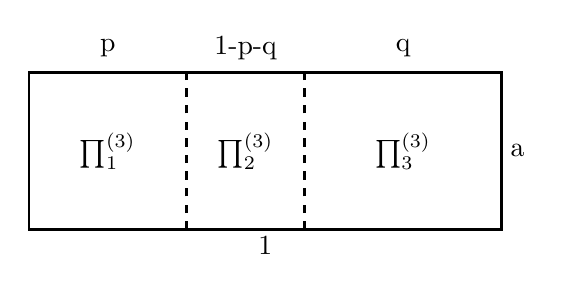
\begin{tikzpicture}[line width=1pt]
        \draw (0,0) rectangle (6,2);
        \draw [dashed](2,0)--(2,2);
        \draw [dashed] (3.5,0)--(3.5,2);
        \node at (3,-0.2) {1};
        \node at (6.2,1){a};
        \node at (1,2.3){p};
        \node at (2.75,2.3){1-p-q};
        \node at (4.75,2.3){q};
        \node at (1,1){$\prod_1^{(3)}$};
        \node at (2.75,1){$\prod_2^{(3)}$};
        \node at (4.75,1){$\prod_3^{(3)}$};
    \end{tikzpicture}
    \caption{}
\end{figure}

    
%\begin{figure}
    %\centering
    %\includegraphics[width=0.7\linewidth]{2.2.jpg}
    %\caption{}
   % \label{fig:enter-label}
%\end{figure}





Assume that the Carath\'{e}odory and Kobayashi metrics agree on the disk $\tau^{\phi_3(a,b,c,p,q)}$, for some choice of $p,q>0$. Let $\phi_3:\tau_{0,6}\rightarrow \mathbb{H}$ be the function from Lemma 5.17
 corresponding to $p$ and $q$.
 
The function $\phi_3$ is holomorphic and $S_3(t,h)$ is infinitely differentiable about $t$ and $h$, so the function $\phi_3(S_3(t,h))$ is a complex-valued smooth function of $t$ and $h$. Thus $$\phi_3(S_3(t,h))=\phi_3(S_3(0,0))+\delta_1t+\delta_2h+\delta_{11}t^2+\delta_{12}th+\delta_{22}h^2+O((t+h)^3).$$

By the above, we have the following Lemma:

\begin{Lemma}
Let $a,q,q_1,p,p_1$ be such that $q>q_1,p>p_1$, and denote by $\phi_3$ the holomorphic function from Lemma 5.17 corresponding to $q$ and $p$. There exsit $T_1, T_2, T_{11}, T_{12},T_{22},T_{21}$  where $T_{22}\neq0$  such that

\begin{align*}
\phi_3(S_3(a,0,a,p_1,q_1))=&\phi_3(S_3(a,0,a,p,q))+ T   _1\frac{t}{\log t^{-1}}+T_2\frac{h}{\log h^{-1}}+\\& T_{11}\frac{t^2}{\log t^{-1}}+T_{22}\frac{h^2}{\log h^{-1}}+T_{12}\frac{th}{\log t^{-1}}+T_{21}\frac{th}{\log h^{-1}}+\\&o(\frac{t^2}{\log t^{-1}})+o(\frac{h^2}{\log h^{-1}})+o(\frac{th}{\log t^{-1}})+o(\frac{th}{\log h^{-1}})
\end{align*}
where $t=p-p_1, h=q-q_1$.
\end{Lemma}

Proof: Given $a,p_1$ and $q_1$, we find $-1<\xi_1<\xi_2<\xi_3<1$ such that the Schwarz-Christoffel map $f=f(\xi_3,\xi_2,\xi_2,\xi_1,\xi_1)$ maps $\mathbb{H}$ onto $S_3(a,0,a,p_1,q_1)$. We consider $S_3(a(m,s),b(m,s),c(m,s),p(m,s),q(m,s))$. Observe that $p(m,s)$ is increase with $m$ and $q(m,s)$ is increase with  $s$.

We locate the time $m,s$ such that $p=p(m,s)$ and $q=q(m,s)$.
That are $$p-p_1=t=p_1'm\log m^{-1}+o(m\log m^{-1})+O(s)$$
    $$q-q_1=h=q_1's\log s^{-1}+o(s\log s^{-1})+O(m). $$ for some $q_1'>0,p_1'>0$. 
    Thus we obtain $$m=\frac{(1+o(1))t}{p_1'\log t^{-1}}, \log m^{-1}=(1+o(1))\log t^{-1}$$ and $$s=\frac{(1+o(1))h}{q_1'\log {h^{-1}}}, \log s^{-1}=(1+o(1))\log h^{-1}.$$ 

    Since by construction $S_3(a,0,a,p_1,q_1)=S_3(a(m,s),b(m,s),c(m,s),p(m,s),q(m,s))$ in $\tau_{0,6}$. By Lemma 5.17  we find that 
    \begin{align*}  \phi_3(S_3(a,0,a,p_1,q_1))&=\phi_3(S_3(a(m,s),b(m,s),c(m,s),p(m,s),q(m,s)))\\&=iArea(L_3(a(m,s),b(m,s),c(m,s),p(m,s),q(m,s)))
    \end{align*}
On the other hand, we have $a=a(0,0)$ and so $\Phi(S_3(a(0,0),0,a,p,q)=a(0,0)$.
It follows that 
\begin{align*}
    \phi_3(S_3(a,0,a,p_1,q_1))-\phi_3(S_3(a(0,0),0,a,p,q)=&i[Area(L_3(a(m,s),b(m,s),c(m,s),\\&p(m,s),q(m,s)))-a(0,0)]
\end{align*}


By Proposition 5.21, replacing $m$ and $s$ with $t$ and $h$, we can get the desired equality.

\begin{Theorem}
    The Carath\'{e}odory metric and Kobayashi metric is not agree on the Teichm\"{u}ller disk $\tau^{\phi_3(a,b,c,p,q)}$ for any choices of $a,b,c,p,q$.
\end{Theorem}
Proof: Suppose not.
By Lemma 5.22 and Lemma 5.23, we have 
\begin{align*}
  \delta_1t+\delta_2h+\delta_{11}t^2+\delta_{12}th+\delta_{22}h^2+O((t+h)^3)=&T_1\frac{t}{\log t^{-1}}+T_2\frac{h}{\log h^{-1}}+\\& T_{11}\frac{t^2}{\log t^{-1}}+T_{22}\frac{h^2}{\log h^{-1}}+\\&T_{12}\frac{th}{\log t^{-1}}+T_{21}\frac{th}{\log h^{-1}}+\\&o(\frac{t^2}{\log t^{-1}})+o(\frac{h^2}{\log h^{-1}})+\\&o(\frac{th}{\log t^{-1}})+o(\frac{th}{\log h^{-1}})
\end{align*}

 Firstly, we make $h=0$ and let $t\rightarrow0$. We can get $\delta_1=0$ and $T_1=0$. Secondly,  we make $t=0$ and let $h\rightarrow0$, we can get $\delta_2=0$ and $T_2=0$. Thirdly, let $t=0$ again. 
 We have 
 $$\delta_{22}h^2+O(h^3)=T_{22}\frac{h^2}{\log h^{-1}}+o(\frac{h^2}{\log h^{-1}}).$$

Dividing both two sides of the above equality by $\frac{h^2}{\log h^{-1}}$, we get 
 $$\delta_{22}\log h^{-1}+O(h\log h^{-1})=T_{22}+o(1).$$ Let $h\rightarrow0$, we must have $\delta_{22}=T_{22}=0$, which contradicts to Lemma 5.23.
 


 
 
 
 %Let $h=0$ again and $t\rightarrow0$, we can get $\delta_{11}=0$ and $T_{11}=0$.
%Thus $\delta_{12}th+O((t+h)^3)=T_{12}\frac{th}{\log t^{-1}}+T_{21}\frac{th}{\log h^{-1}}+o(\frac{t^2}{\log t^{-1}}+\frac{h^2}{\log h^{-1}})$.
%Let $h=t$ and $t\rightarrow0$, we can easily get $\delta_{12}=T_{12}=T_{21}=0$, which is contradicted to Lemma 4.23.










\begin{figure}
    \centering
    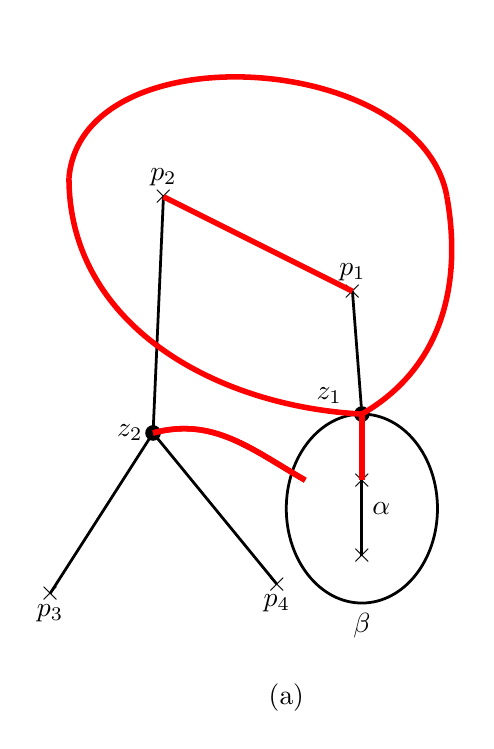
\begin{tikzpicture}[line width=1pt,scale=1.2]
        \draw (0,1)--(-0.11,-1.5)--(-1.2,-3.2);
        \draw (-0.11,-1.5)--(1.2,-3.1);
        \draw (2.1,-2.3) ellipse (0.8cm and 1.0cm);
        \draw (2.1,-1.3)--(2.0,0);
        \draw (2.1,-2)--(2.1,-2.8);
         \node[ circle, fill=black,inner sep = 2pt] (A) at (-0.11,-1.5){};
        \node[ circle, fill=black,inner sep = 2pt] (A) at (2.1,-1.3){};
         \node at(0,1){$\times$}; 
        \node  at(-1.2,-3.2){$\times$};
        \node  at(1.2,-3.1){$\times$}; 
       \node  at(2.0,0){$\times$}; 
        \node  at(2.1,-2){$\times$}; 
        \node  at(2.1,-2.8){$\times$}; 
        \node at (1.3,-4.3) {(a)};
        \node[left] at (-0.11,-1.5) {$z_2$};
        \node[left] at (2,-1.1) {$z_1$};
         \node[above] at(0,1){$p_2$};
         \node[above] at(2,0){$p_1$};
         \node[below] at(-1.2,-3.2){$p_3$};
         \node[below] at(1.2,-3.1){$p_4$};
            \node[below] at(2.1,-3.3){$\beta$};
      \node[right] at(2.1,-2.3){$\alpha$};
              \draw[red,line width=2pt] (0,1)--(2,0);
                 \draw[red,line width=2pt] (2.1,-1.3) to[out=177,in=270] (-1, 1.2);
                 \draw[red,line width=2pt] (-1, 1.2) to[out=85,in=100] (3, 1);
                  \draw[red,line width=2pt] (3,1) to[out=280,in=30] (2.1,-1.3);
       \draw[red,line width=2pt] (2.1,-1.3) -- (2.1,-2);
        \draw[red,line width=2pt] (-0.11,-1.5) to[out=15,in=150] (1.5,-2);
         \draw[red,line width=2pt] (-0.11,-1.5) to[out=15,in=150] (1.5,-2);
    \end{tikzpicture}

\caption{Case (I-7-a). }
       \label{fig:A-7-a} 
\end{figure} 


\begin{figure}[h]
    \centering
    \begin{tikzpicture}[line width=1pt, scale=0.7]
        \draw (0,0) ellipse (1cm and 3cm);
         \draw (0,0) ellipse (3cm and 4cm);
         \node[ circle, fill=black,inner sep = 2pt] (A) at (-1,0){};
        \node[ circle, fill=black,inner sep = 2pt] (A) at (-3,0){};
         \node at (0,0) {$\times$};
         \node at (0,2) {$\times$};
         \node at (0,-2) {$\times$};
         \draw (0,0) -- (-1,0);
         \draw (0,2) .. controls(0.8,0) .. (0,-2);
         \node at (-3,3) {$\times$};
         \node at (-3,-3) {$\times$};
         \node at (-5,0) {$\times$};
         \draw (-3,0) -- (-5,0);
         \draw[line width=2pt, dashed] (-1,0) -- (-3,0);
          \draw (-3,3) .. controls(6,10) and (6,-10) .. (-3,-3);
    \end{tikzpicture}
    \vspace*{-40mm}
    \caption{Case (I-6-b). The graph denotes the vertical critical leaves of $\phi$. The dashed line denotes $\gamma_3$.}
    \label{fig:A-6-b}
\end{figure}





\begin{figure}[h]
    \centering
    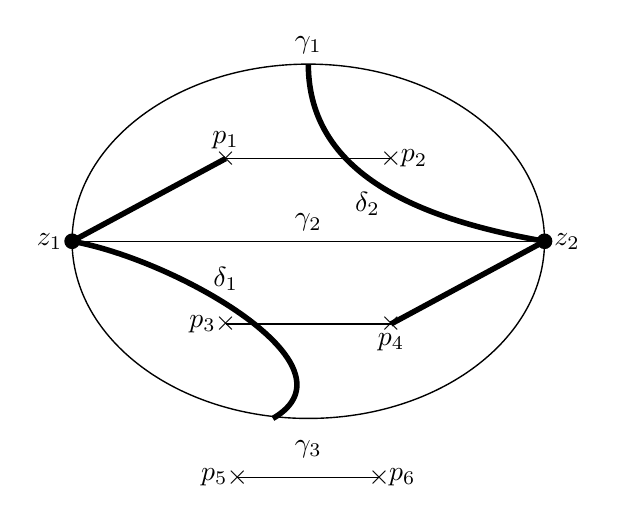
\begin{tikzpicture}[line width=0.5pt, scale=1.5]
        \draw (0,0) ellipse (2cm and 1.5cm);
        \draw (-2,0)--(2,0);
        \draw (-0.7,0.7)--(0.7,0.7);
        \draw (-0.7,-0.7)--(0.7,-0.7);
        \draw (-0.6,-2)--(0.6,-2);
         \node[ circle, fill=black,inner sep = 2pt] (A) at (-2,0){};
        \node[ circle, fill=black,inner sep = 2pt] (A) at (2,0){};
         \node at(-0.7,0.7){$\times$}; 
        \node  at(0.7,0.7){$\times$};
        \node at(-0.7,-0.7){$\times$}; 
       \node at(0.7,-0.7){$\times$}; 
        \node at(-0.6,-2){$\times$}; 
        \node at(0.6,-2){$\times$};
        \node[above] at(-0.7,0.7){$p_1$}; 
        \node[right]  at(0.7,0.7){$p_2$};
        \node[left] at(-0.7,-0.7){$p_3$}; 
       \node[below] at(0.7,-0.7){$p_4$}; 
        \node[left] at(-0.6,-2){$p_5$}; 
        \node[right] at(0.6,-2){$p_6$};
        \node[above] at(0,1.5){$\gamma_1$};
        \node[above] at(0,0){$\gamma_2$};
        \node[below] at(0,-1.6){$\gamma_3$};
        \node[left] at(-2,0) {$z_1$};
         \node[right] at(2,0) {$z_2$};
         \draw[line width=2pt] (-2,0)--(-0.7,0.7);
         \draw[line width=2pt] (2,0)--(0.7,-0.7);
          \draw[line width=2pt] (-2,0) to[out=350,in=30] (-0.3,-1.5);
          \draw[line width=2pt] (2,0) to[out=170,in=270] (0,1.5);
          \node[above] at(-0.7,-0.5) {$\delta_1$};
            \node[below] at(0.5,0.5) {$\delta_2$};
    \end{tikzpicture}
    \caption{Case (I-6-b). Thick lines denote vertical saddle connections.}
    \label{fig:A-6-2}
\end{figure}


\begin{figure}[h]
    \centering
    \begin{tikzpicture}[line width=0.5pt, scale=1.5]
        \draw (0,0) ellipse (2cm and 1.5cm);
        \draw (-2,0)--(2,0);
        \draw (-0.7,0.7)--(0.7,0.7);
        \draw (-0.7,-0.7)--(0.7,-0.7);
        \draw (-0.6,-2)--(0.6,-2);
         \node[ circle, fill=black,inner sep = 2pt] (A) at (-2,0){};
        \node[ circle, fill=black,inner sep = 2pt] (A) at (2,0){};
         \node at(-0.7,0.7){$\times$}; 
        \node  at(0.7,0.7){$\times$};
        \node at(-0.7,-0.7){$\times$}; 
       \node at(0.7,-0.7){$\times$}; 
        \node at(-0.6,-2){$\times$}; 
        \node at(0.6,-2){$\times$};
        \node[below] at(-0.7,0.7){$p_1$}; 
        \node[above]  at(0.7,0.7){$p_2$};
        \node[below] at(-0.7,-0.7){$p_3$}; 
       \node[below] at(0.7,-0.7){$p_4$}; 
        \node[left] at(-0.6,-2){$p_5$}; 
        \node[right] at(0.6,-2){$p_6$};
        \node[above] at(0,1.5){$\gamma_1$};
        \node[above] at(0,0){$\gamma_2$};
        \node[below] at(0,-1.6){$\gamma_3$};
        \node[left] at(-2,0) {$z_1$};
         \node[right] at(2,0) {$z_2$};
         \draw[line width=2pt] (-2,0)--(-0.7,0.7);
         \draw[line width=2pt] (2,0)-- (0.7,0.7);
               \draw[line width=2pt] (2,0) .. controls (5,3) and (4,-6) .. (0.4,-2);
             \draw[line width=2pt] (-2,0) .. controls (-5,3) and (-4,-6) .. (-0.4,-2);
         \draw[line width=2pt] (-2,0) .. controls (-0.2,-0.7) .. (-0.4,-2);
          \draw[line width=2pt] (2,0) .. controls (0.2,-0.7) .. (0.4,-2);
          %\draw[line width=2pt] (-2,0) to[out=350,in=30] (-0.3,-1.5);
          %\draw[line width=2pt] (2,0) to[out=170,in=270] (0,1.5);
          %\node[above] at(-0.7,-0.5) {$\delta_1$};
          %  \node[below] at(0.5,0.5) {$\delta_2$};
    \end{tikzpicture}
    \caption{Case (I-6-c). Thick lines denote vertical saddle connections.}
    \label{fig:A-6-3}
\end{figure}

\begin{figure}[h]
    \centering
    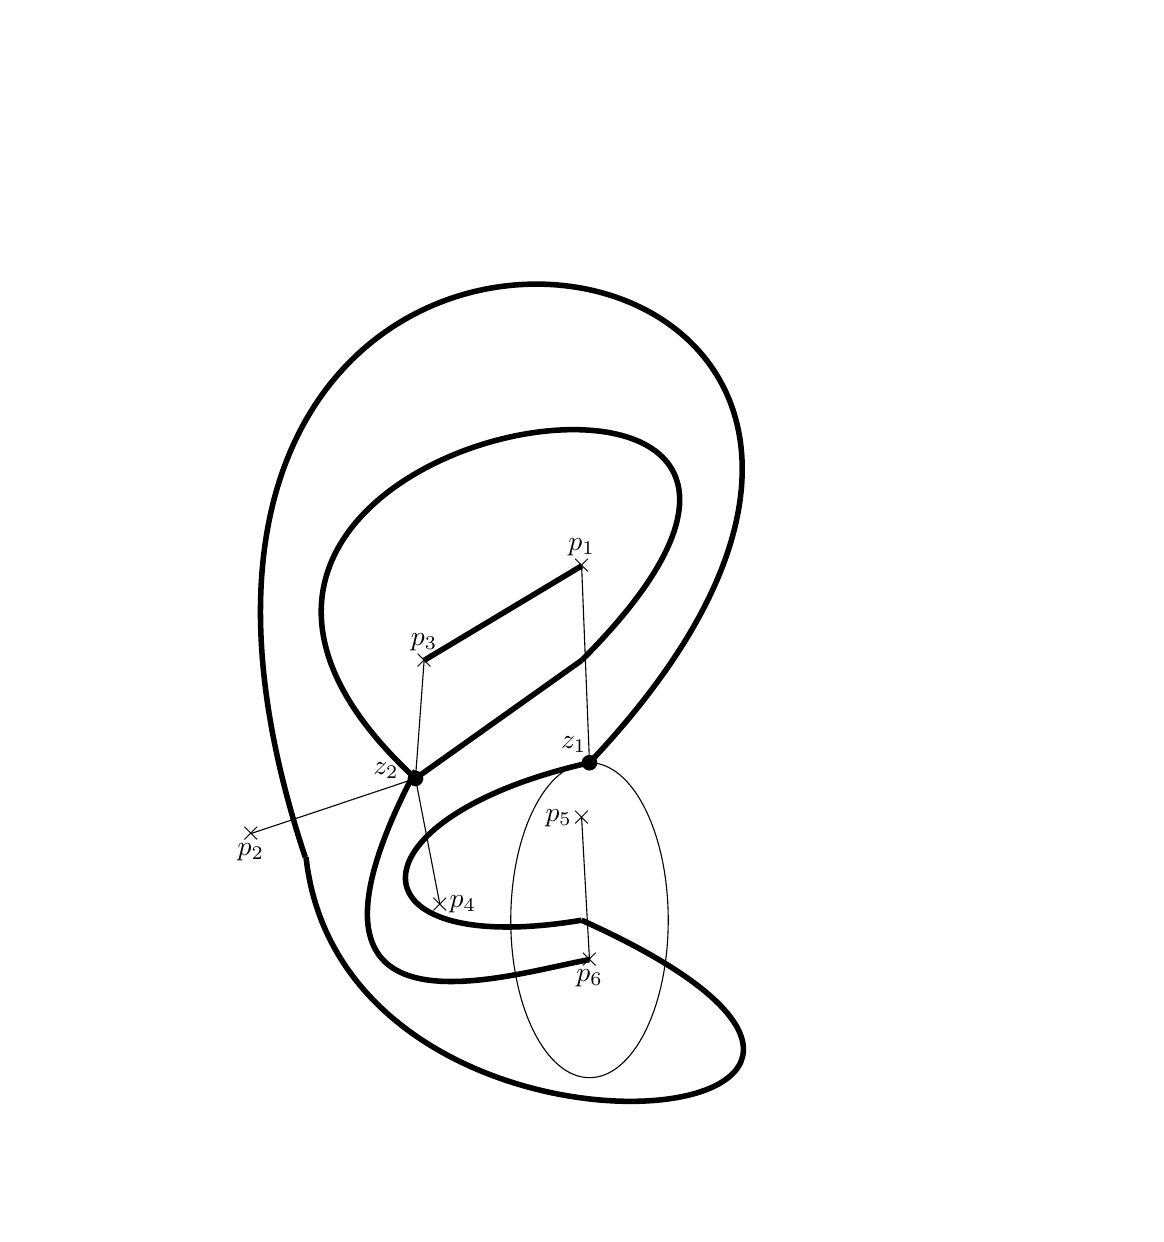
\begin{tikzpicture}[scale=1]
        \draw (0,0)--(-0.11,-1.5)--(-2.2,-2.2);
        \draw (-0.11,-1.5)--(0.2,-3.1);
        \draw (2.1,-3.3) ellipse (1cm and 2cm);
        \draw (2.1,-1.3)--(2.0,1.2);
        \draw (2,-2)--(2.1,-3.8);
         \node[ circle, fill=black,inner sep = 2pt] (A) at (-0.11,-1.5){};
        \node[ circle, fill=black,inner sep = 2pt] (A) at (2.1,-1.3){};
         \node at(0,0){$\times$}; 
        \node  at(-2.2,-2.2){$\times$};
        \node  at(0.2,-3.1){$\times$}; 
       \node  at(2.0,1.2){$\times$}; 
        \node  at(2,-2){$\times$}; 
        \node  at(2.1,-3.8){$\times$}; 
        \node[left] at (-0.2,-1.4) {$z_2$};
        \node[above] at (1.9,-1.3) {$z_1$};
         \node[above] at(0,0){$p_3$};
         \node[above] at(2,1.2){$p_1$};
           \node[left] at(2,-2){$p_5$};
             \node[below] at(2.1,-3.8){$p_6$};
         \node[below] at(-2.2,-2.2){$p_2$};
         \node[right] at(0.2,-3.1){$p_4$};
      \draw[line width=2pt](-0.11,-1.4) .. controls (-2,-5) and (1,-4) .. (2.1,-3.8);
      \draw[line width=2pt] (2,1.2) -- (0,0);
        \draw[line width=2pt]  (-0.11,-1.5) -- (2,0);
         \draw[line width=2pt] (2,0)  .. controls (7,5) and (-5,3) .. (-0.11,-1.5);
            \draw[line width=2pt] (2.1,-1.3)  .. controls (9,6) and (-5,8) .. (-1.51,-2.5);
         \draw[line width=2pt] (2,-3.3)  .. controls (8,-6) and (-1,-7) .. (-1.5,-2.5);
      \draw[line width=2pt] (2,-3.3)  .. controls (-1,-3.8) and (-1,-2) .. (2.1,-1.3);
    \end{tikzpicture}
\caption{Thick lines denote vertical leaves. There is a vertical cylinder with close leaves surrounding $\widehat{p_2p_6}$ and bounded by $\delta$. }
       \label{fig:A-7-2} 
\end{figure}




\end{comment}









%%%%%%%%%%%%%%%%%%%%%%%%%%%%%%%%%%%%%%%%%%%%%%%%%%%%%%%%%%%%%%%%%%%%%%%%%%%%%%%%%%%%%%%%%%%%%%%%%%%%%%%%%%%%%%%%%%%%%%%%%%%%%%%%%%%%%%%%%%%%%%%%%%%%%%%%%%%%%%%%%%%%%%%%%%%%%%5


\bibliographystyle{plain}

\bibliography{bibliography}



    
\end{document}



 \begin{figure}[h]
    \centering
    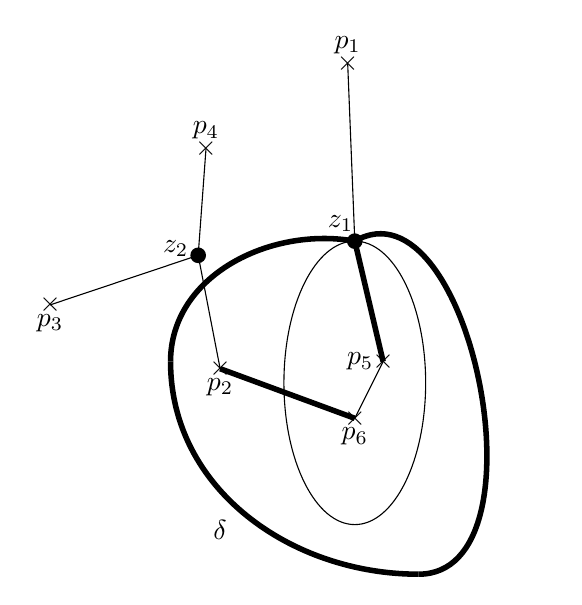
\begin{tikzpicture}[scale=0.9]
        \draw (0,0)--(-0.11,-1.5)--(-2.2,-2.2);
        \draw (-0.11,-1.5)--(0.2,-3.1);
        \draw (2.1,-3.3) ellipse (1cm and 2cm);
        \draw (2.1,-1.3)--(2.0,1.2);
        \draw (2.5,-3)--(2.1,-3.8);
         \node[ circle, fill=black,inner sep = 2pt] (A) at (-0.11,-1.5){};
        \node[ circle, fill=black,inner sep = 2pt] (A) at (2.1,-1.3){};
         \node at(0,0){$\times$}; 
        \node  at(-2.2,-2.2){$\times$};
        \node  at(0.2,-3.1){$\times$}; 
       \node  at(2.0,1.2){$\times$}; 
        \node  at(2.5,-3){$\times$}; 
        \node  at(2.1,-3.8){$\times$}; 
        \node[left] at (-0.11,-1.4) {$z_2$};
        \node[above] at (1.9,-1.3) {$z_1$};
         \node[above] at(0,0){$p_4$};
         \node[above] at(2,1.2){$p_1$};
           \node[left] at(2.5,-3){$p_5$};
             \node[below] at(2.1,-3.8){$p_6$};
         \node[below] at(-2.2,-2.2){$p_3$};
         \node[below] at(0.2,-3.1){$p_2$};
          \draw[line width=2pt] (0.2,-3.1) -- (2.1,-3.8);
          \draw[line width=2pt] (2.1,-1.3) -- (2.5,-3);
      \draw[line width=2pt] (2.1,-1.3) to[out=170,in=90] (-0.5, -3);
       \draw[line width=2pt](-0.5, -3) to[out=270,in=180] (3, -6);
       \draw[line width=2pt](3,-6) to[out=0,in=30] (2.1,-1.3);
       \node[below] at(0.2,-5.1){$\delta$};
    \end{tikzpicture}
\caption{Thick lines denote vertical leaves. There is a vertical cylinder with close leaves surrounding $\widehat{p_2p_6}$ and bounded by $\delta$. }
       \label{fig:I-7-2} 
\end{figure}
